\documentclass{article}
\usepackage{tikz}
\usepackage{pgfplots}
% Ajustes de pgfplots
\pgfplotsset{compat=1.18}  % sin width aquí
% Librerías de pgfplots (DESPUÉS de \usepackage{pgfplots})
\usepgfplotslibrary{groupplots}
\usepgfplotslibrary{statistics}
\usetikzlibrary{angles, quotes}
\usepackage{amssymb}
\pgfplotsset{width=10cm,compat=1.9}
\usepackage[left=2.54cm,right=2.54cm,top=2.54cm,bottom=2.54cm]{geometry}
\usepackage{tasks} %Paquete necesario para la producción de items horizontales para algunos ejercicios de tarea empleando el comando /begin{multicols}}{#}.../end{multicols} para ayudarnos a reducir las páginas
\usepackage{pdflscape} %comando que permite cambiar a orientación horizontal las hojas%
\usepackage{soul} %Paquete para permitir la compilación de acentos usando el comando {\hl{}}}\\
\sethlcolor{yellow(munsell)} %comando para definir el color para el subrayado usando el comando \hl
\usepackage[utf8]{inputenc}
\usepackage[spanish]{babel}
\usepackage{icomma}
\usepackage{ragged2e}		
\usepackage{siunitx}
\usepackage{url}
\usepackage[colorlinks=true, urlcolor=blue,  linkcolor=Cerulean, citecolor=green]{hyperref}
\usepackage{pdfpages}
\usepackage{blindtext} %Paquete que genera texto ficticio (dummy text) con el comando: \blindtext
\usepackage{cancel} %in the preamble gives you four different modes of striking through: \cancel{text to cancel} draws a diagonal line (slash) through its argument, \bcancel{text to cancel} uses the negative slope (a backslash), \xcancel{text to cancel} draws an X (actually \cancel plus \bcancel), \cancelto{〈value〉}{〈expression〉} draws a diagonal arrow through the 〈expression〉pointing to the 〈value〉 (math-mode only)
\usepackage{csquotes}
\usepackage{afterpage}
\usepackage{parskip} 
\usepackage{float}
\usepackage{enumitem}
%\usepackage{multicol}%Paquete que permite la creación aislada de columnas de texto. De esta forma se reduce la cantidad de páginas en nuestro documento
\usepackage{lipsum} %Paquete que genera texto de relleno al igual que \usepackage{blindtext}, se usa con el comando \lipsum[#-#] los #(hashtags) delimitan el número de páginas que deseamos ocupar del paquete lipsum para usarlos como relleno. 

% Definir el comando personalizado para la nota
\newcommand{\mynote}[1]{%
\begin{tikzpicture}[baseline=-0.75ex]
\node[draw, circle, fill=Apple Green!60, inner sep=2pt] (note) {\textbf{Nota:}};
\end{tikzpicture}%
\ \textit{#1}%
}

% Definición de comandos para variables con barra
\newcommand{\xbar}{\overline{x}}
\newcommand{\ybar}{\overline{y}}

\newenvironment{Figura}
{\par\medskip\noindent\minipage{\linewidth}}
{\endminipage\par\medskip}
\usepackage{caption}
\usepackage[
backend=biber,
sorting=none,
url=true
]{biblatex} %bibliografía
\addbibresource{biblio.bib}
% Establecer el espacio entre las entradas de la bibliografía
\setlength{\bibitemsep}{1\baselineskip} % Puedes ajustar el valor según tus preferencias
\usepackage{amsmath,amsthm,amssymb,amsfonts}
\usepackage{pifont} %Permite la compilación del comando \xmark: es el símbolo de la tachita
\usepackage{mathtools} %permite la compilación de símbolos para matrices
\usepackage{empheq} %Paquete que se relaciona con \usepackage[most]{tcolorbox} para la creación de cuadros/cajas de colores para delimitar los resultados matemáticos o líneas de texto usando la línea de comando: \begin{empheq}[box={\mymath[colback=orange(webcolor)!70,drop lifted shadow]}]{equation*} \end{empheq}
\usepackage[most]{tcolorbox} %Paquete que se relaciona con \usepackage{empheq} para la creación de cuadros/cajas de colores para delimitar los resultados matemáticos o líneas de texto
\renewcommand{\qedsymbol}{$\blacksquare$}
\usetikzlibrary{positioning,decorations.pathreplacing} %Paquete que permite la compilación de llaves para cuadros sinópticos (brace diagram) 
\usepackage{schemata} %The schemata package is designed just for these brace diagrams
\usepackage{booktabs}

\newcommand\AB[2]{\schema{\schemabox{#1}}{\schemabox{#2}}} %comando o paquete necesario para crear cuadros sinópticos

\newtcbox{\mymath}[1][]{%
nobeforeafter, math upper, tcbox raise base,
enhanced, colframe=blue!30!black,
colback=blue!30, boxrule=1pt,
#1} %Comando importante para encasillar los resultados matemáticos en cajas de diferentes colores, se relaciona con los paquetes \usepackage{empheq} y \usepackage[most]{tcolorbox} 

\newenvironment{sysmatrix}[1]
{\left(\begin{array}{@{}#1@{}}}
{\end{array}\right)}
\newcommand{\ro}[1]{%
\xrightarrow{\mathmakebox[\rowidth]{#1}}%
}
\newlength{\rowidth}% row operation width
\AtBeginDocument{\setlength{\rowidth}{3em}}  %Comando importante para laproducción de lineas de operaciones entre matrices, método de Gauss o Gauss Jordan se relaciona con \newenvironment{sysmatrix}

%formato para cambiar el horario a español
\usepackage[spanish]{datetime2}
\DTMsetdatestyle{spanish}

\renewcommand{\today}{\DTMdisplaydate{\the\year}{\the\month}{\the\day }{-1}}
%%%%%%%%%%%%%%%%%%%%%%%%%%%%%%%%%%%%%%%%%

\usepackage{datetime}
\newcommand{\mycurrenttime}{\xxivtime}

%%%%%%%%%%%%%%%%%%%%%%%%%%%%%%%%%%%%%%%%%%%%%%%%%%%%%%%%%%%%%%%%%%%%%%%%%%%%%%%%%%%%%%%%%%%%%%%%%%%%%%%%%%%%%%%%%%%%%%%%%%%%%%%%%%%%%%%%%%%%%%%%%


%%%%%%%%%%%%%Caja de color para el título%%%%%%%%%%%%%%%%%%%%%%%%%%%%%%%%%%%%%%%%%%%%%%%%%%%%%%

\definecolor{myframecolor}{RGB}{1, 45, 75} % Prussian Blue
\definecolor{myboxcolor}{RGB}{0, 107, 92} % Apple Green

\newtcolorbox{mybox}{
enhanced,
colback=myboxcolor!7, % Color de fondo del cuadro
colframe=myframecolor, % Color del marco del cuadro
arc=0pt,
boxrule=1pt,
borderline west={2mm}{-10mm}{myframecolor}, % Borde en el lado izquierdo
sharp corners=southwest,
width=\linewidth,
before=\par\vspace{\bigskipamount}, % Espacio antes del cuadro
after=\par\vspace{\bigskipamount} % Espacio después del cuadro
}

%%%%%%%%%%%%%%%%%%%%%%%%%%%%%%%%%%%%%%%%%%%%%%%%%%%%%%%%%Nueva caja%%%%%%%%%%%%%%%%%%%%%%%%%%%%%%%%%%%%%%%%%%%%%%%%%%%%%%%%%%%%%%%%%

\newtcolorbox{mybox2}{
enhanced,
colback=Apple Green!7, % Color de fondo del cuadro
colframe=Apple Green, % Color del marco del cuadro
arc=0pt,
boxrule=1pt,
borderline west={2mm}{-10mm}{Apple Green}, % Borde en el lado izquierdo
sharp corners=southwest,
width=\linewidth,
before=\par\vspace{\bigskipamount}, % Espacio antes del cuadro
after=\par\vspace{\bigskipamount} % Espacio después del cuadro
}


\newcommand{\euler}{e} %Comando para producir letra e de euler
\newenvironment{remark}{\par\vfill\footnotesize % Vertical white space above the remark and smaller font size
\begin{list}{}{
	\leftmargin=80pt % Indentation on the left
	\rightmargin=60pt}\item\ignorespaces % Indentation on the right
\makebox[-2.5pt]{\begin{tikzpicture}[overlay]
		\node[draw=Horizon!60,line width=2.5pt,circle,fill=Horizon!25,font=\sffamily\bfseries,inner sep=4pt,outer sep=0pt] at (-19pt,5pt){\textcolor{Horizon}{Nota}};\end{tikzpicture}} % Blue Nota in a circle
\advance\baselineskip -1pt}{\end{list}\vskip5pt} % Tighter line spacing and white space after remark
\usepackage{graphicx}

\usepackage{titling}

\input{colores.tex}

%%Producir signos de cita textual``Asignatura''

\newcommand{\xmark}{\ding{55}} %%%comando que genera la tachita

\newenvironment{MyColorPar}[1]{%
\leavevmode\color{#1}\ignorespaces%
}{%
}%

%%%%%%%%%%%%%%%%%%% Título de la tarea, Nombre de alumno

\title{ \textcolor{Sun}{\textbf{Ejercicios}}}
\author{\emph{Tarea 4} $\boldsymbol{\mid}$ \textcolor{Tarawera}{\textbf{Ecuaciones de Hamilton}}}
\date{\today}

%%%%%%%%%%%%%%%%%%% Datos de la Materia

\usepackage{fancyhdr}
\fancypagestyle{plain}{%  the preset of fancyhdr 
\fancyhf{} % clear all header and footer fields
\fancyfoot[R]{
\includegraphics[width=2cm]{LogoFCFMBUAP (1).png}}
\fancyfoot[L]{{\bfseries{\thedate{}}} a las {\bfseries{\mycurrenttime{}}} horas{} (GMT-6, H. Puebla de Zaragoza, Pue)}
\fancyhead[L]{\textbf{Asignatura:} Mecánica Teórica}
\fancyhead[R]{\theauthor}
}
\makeatletter
\def\@maketitle{%
\newpage
\null%
\begin{center}%
\let \footnote \thanks
{\LARGE \@title \par}%
\vskip 1em%
%{\large \@date}%
\end{center}%
}
\makeatother

\usepackage{lipsum}  
\usepackage{cmbright}


%%%%%%%%%%%%%%%%%%%%%%%%%%%%%%%%%%%%%%%%%%%%%%%%%%%%%%%%%%%%%%%%%%%%%%%%%%%%%%%%%%%%%%%%%%%%%%%%%%%%%%%%%%%%%%%%%%%%%%%%%%%%%%%%%%%%%%%%%%%%%%%%%%%%%%%%%%%%%%%%%%%%%%%%%%%%%%%%%%%%%%%%%%%%%%%%%%%%%%

% Por si el color se llama "Apple Green" con espacio en colores.tex:
\colorlet{AppleGreen}{Apple Green}

% Caja AppleGreen con tono ajustable
\newenvironment{AGbox}[1][7]% 7 = tono por defecto (más grande => más claro)
{%
  \begin{tcolorbox}[
    enhanced, breakable,
    colframe=AppleGreen,
    colback=AppleGreen!#1,
    boxrule=1pt,
    borderline west={2mm}{-10mm}{AppleGreen},
    sharp corners=southwest,
    left=14pt,right=14pt,top=10pt,bottom=10pt,
     boxsep=6pt,
  ]%
}{%
  \end{tcolorbox}%
}


\begin{document}



\maketitle

%%%%%%%%%%%%%%%%%%% Datos del profesor, campus, aula e integrantes

\begin{mybox2}
\noindent
\begin{tabular}{@{}p{3.7cm}p{10.4cm}@{}}
\textbf{Profesor} & Dr. Gilberto Silva Ortigoza \\[3pt]
\textbf{Campus / Facultad} & \textcolor{prussianblue}{\textbf{C.U. BUAP}} / \textcolor{trueblue}{\textbf{FCFM}} \\[3pt]
\textbf{Edificio / Salón} & \textcolor{prussianblue}{\textbf{EMA4}} / \textcolor{trueblue}{\textbf{302}} \\[6pt]
\textbf{Integrantes} &
\begin{minipage}[t]{\linewidth}
\raggedright
\textbf{González-Salud}, S.\textsuperscript{1};\,
\textbf{Victoria-García}, A. A.\textsuperscript{2};\,
\textbf{Cruz-Toledo}, F. A.\textsuperscript{3};\,
\textbf{Calderón-Muñoz}, J. C.\textsuperscript{(oyente)4};\,
\textbf{Gómez-González}, F. S.\textsuperscript{5};\,
\textbf{Hernández-Mejía}, M. I.\textsuperscript{6};\,
\textbf{Torres-Luna}, N. A.\textsuperscript{7};\,
\textbf{Martínez-Solorio}, R. J.\textsuperscript{8};\,
\textbf{Arroyo-Gonzalez}, D.\textsuperscript{9};\,
\textbf{Sandoval-Zonotl}, H.\textsuperscript{10};\,
\textbf{Peralta-Rebolledo}, A.\textsuperscript{11};\,
\textbf{Gómez-Alatorre}, A. D.\textsuperscript{12};\,
\textbf{Ballinas-García}, J. A.\textsuperscript{13}
\end{minipage}
\end{tabular}
\end{mybox2}
\vspace{1cm}


\vspace{0.5cm}
\begin{center}
\begin{tikzpicture}
	% Dibuja círculos rellenos en diferentes colores
	\fill[bittersweet] (0,0) circle (0.17cm);
	\fill[Apple Green] (0.6,0) circle (0.17cm);
	\fill[trueblue] (1.2,0) circle (0.17cm);
	\fill[Aguamarina] (1.8,0) circle (0.17cm);
	\fill[Sun] (2.4,0) circle (0.17cm);
	\fill[orange(colorwheel)] (3.0,0) circle (0.17cm);
	\fill[Pesto] (3.6,0) circle (0.17cm);
	\fill[blue-violet] (4.2,0) circle (0.17cm);
	\fill[ticklemepink] (4.8,0) circle (0.17cm);
	\fill[Gallery] (5.4,0) circle (0.17cm);
	\fill[Mantle] (6.0,0) circle (0.17cm);
	\fill[Nevada] (6.6,0) circle (0.17cm);
	\fill[onyx] (7.2,0) circle (0.17cm);
	% Agrega más círculos o modifica los colores según sea necesario
\end{tikzpicture}
\end{center}  \vspace{0.5cm}

\section*{\textcolor{Tarawera}{\textbf{Lista de problemas y soluciones}}}
\addcontentsline{toc}{section}{\textcolor{Tarawera}{\textbf{Problemas: cap 3}}}

\setlength{\columnsep}{2cm}
%\begin{multicols}{2}

%=============================
% PR. 4.1
%=============================
\begin{AGbox}[8]
\begin{enumerate}[label={{\textcolor{trueblue}{\textbf{Pr.} 4.1}}}]
  \item Sea $F(x,p) = px - x^{2}/2$, una función de las variable $x$ y $p$. (a) En tres dimensiones presentar la gráfica de $F(x,p)$. (b) Supongamos que $p = p_{0}$, donde $p_{0}$ está dado; es decir es fijo, de esta forma definimos $F_{p_{0}}(x) \equiv p_{0}x - x^{2}/2$, la cual es una función de la variable $x$, a continuación generamos el conjunto de funciones $\{F_{p_{0}}(x)\}_{p_{0}=10}^{p_{0}=-10}$; es decir, el conjunto de 21 funciones, ahora en un solo gráfico, en dos dimensiones, presente las gráficas de estas 21 funciones. Hacer los mismo para la función $F(x,p) = px - x^{3}/3$.
\end{enumerate}
\end{AGbox}
\vspace{0.5cm}

\textcolor{Cinnabar}{\textbf{Solución:}} \vspace{0.5cm}

Antes de entrar a los detalles geométricos de las gráficas, es útil remarcar que las
funciones del tipo
\[
F(x,p) = px - f(x)
\]
aparecen de manera natural en el \textbf{Capítulo IV} cuando se introduce la
\textcolor{trueblue}{\textbf{transformada de Legendre}}.  
En ese contexto, si partimos de una función \(f(x)\), se construye
\begin{equation}
\begin{split}
F(x,p) &= px - f(x)
\end{split}\label{eq:legendre-general}
\end{equation}
y luego se busca el \textbf{extremo} de \(F\) con respecto a la variable \(x\), manteniendo
\(p\) fijo  
\[
\frac{\partial F}{\partial x} = 0 \quad \to p = \frac{ df(x)}{dx}
\]

\emph{``Sí de esta última ecuación es posible obtener la variable $x$ en términos de la nueva variable $p$; es decir,''}



\[x=x(p)\]

\emph{``Entonces la transformada de Legendre de la función  $f(x)$, está definida por la siguiente ecuación''}

\[ g(p) \equiv F(x(p),p) = px(p) - f(x(p)) \]


En este roblema, \(f(x)\) será \(x^{2}/2\) o \(x^{3}/3\), de modo que la estructura de
Legendre está presente en estum porblema.



\vspace{0.5cm}

Comenzamos analizando la función \(F\), la cual está definida como:
\[
F:\mathbb{R}^{2}\longrightarrow \mathbb{R},
\]
cuyas variables independientes son \((x,p)\in\mathbb{R}^{2}\) y cuyo valor es

\begin{equation}
\begin{split}
F(x,p) &= px - \frac{x^{2}}{2}
\end{split}\label{eq:F-cuadratica}
\end{equation}

Aunque el dominio de la función es el plano \((x,p)\in\mathbb{R}^{2}\), la \textbf{gráfica} de la función es el conjunto de puntos
\[
(x,p,F(x,p)) \in \mathbb{R}^{3},
\]
de modo que a cada punto \((x,p)\) del plano se le asigna una “altura” dada por el valor de \(F(x,p)\) en \eqref{eq:F-cuadratica}.  
Esta gráfica es una superficie en el espacio tridimensional con coordenadas \((x,p,F)\).

En la notación general de la transformación de Legendre \eqref{eq:legendre-general}, aquí podemos identificar

\begin{equation}
\begin{split}
f(x) &= \frac{x^{2}}{2}
\end{split}\label{eq:f-cuadratica}
\end{equation}

de modo que \(F(x,p)\) adopta la forma:

\begin{equation}
\begin{split}
F(x,p) &= p\,x - f(x)
\end{split}\label{eq:F-cuadratica-legendre}
\end{equation}


%-------------------- Parte (a): gráfica 3D de F(x,p) cuadrática --------------------

\vspace{0.3cm}
\textbf{(a) Gráfica en tres dimensiones de $F(x,p) = px - x^{2}/2$}

Para comprender de manera clara la forma de la superficie definida por
\[
F:\mathbb{R}^{2}\longrightarrow\mathbb{R},
\qquad (x,p)\longmapsto F(x,p)
\]
es útil empezar recordando que la función tiene la estructura general
\begin{equation}
\begin{split}
F(x,p) &= p\,x - f(x)
\end{split}\label{eq:F-general-legendre-again}
\end{equation}
donde, para el caso cuadrático que nos interesa,
\begin{equation}
\begin{split}
f(x) &= \frac{x^{2}}{2}
\end{split}\label{eq:f-cuadratica-again}
\end{equation}
Sustituir \eqref{eq:f-cuadratica-again} en \eqref{eq:F-general-legendre-again} nos conduce a la expresión explícita
\begin{equation}
\begin{split}
F(x,p) &= p\,x - \frac{x^{2}}{2}
\end{split}\label{eq:F-cuadratica-explicita-again}
\end{equation}

\vspace{0.25cm}
\textcolor{trueblue}{\textbf{Descripción geométrica a partir del gráfico 3D}}

La superficie de \eqref{eq:F-cuadratica-explicita-again} se representó en un sistema
de coordenadas tridimensional \((x,p,F)\) empleando \texttt{Python} y la librería
\texttt{Plotly}.  
En la figura se dibuja:

\begin{itemize}
  \item[$\bullet$] La \textbf{superficie} $F(x,p)=px-x^{2}/2$ como una lámina continua de color tipo \emph{Viridis}  
  \item[$\bullet$] El \textbf{plano de referencia} $F=0$ como una malla rectangular gris  
  \item[$\bullet$] Los \textbf{ejes coordenados}: eje $x$ en rojo, eje $p$ en azul y eje $F$ en verde, todos pasando por el origen
\end{itemize}

Para apreciar mejor la geometría, se generaron varias vistas de la misma superficie:

\begin{figure}[H]
\centering
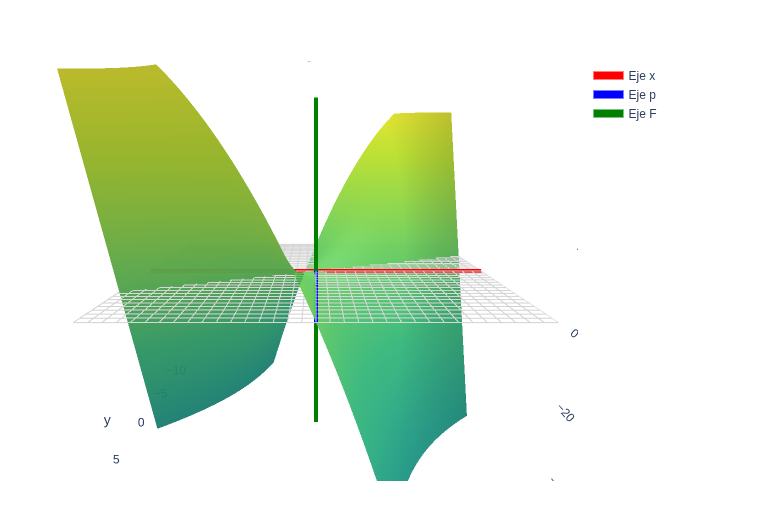
\includegraphics[width=0.75\textwidth]{frontal.png}
\caption{Vista \textbf{frontal} de la superficie $F(x,p) = px - x^{2}/2$, donde se distingue claramente la apertura parabólica en la dirección de $x$ y la posición del plano $F=0$}
\label{fig:Fxp_frontal}
\end{figure}

\begin{figure}[H]
\centering
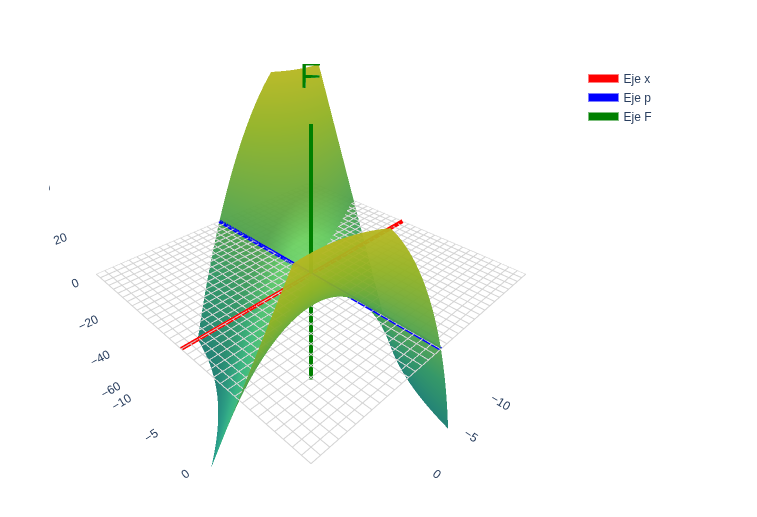
\includegraphics[width=0.75\textwidth]{isométrica.png}
\caption{Vista \textbf{isométrica} de la superficie, mostrando simultáneamente la dependencia en $x$ y en $p$, así como la intersección con el plano $F=0$}
\label{fig:Fxp_isometrica}
\end{figure}

\begin{figure}[H]
\centering
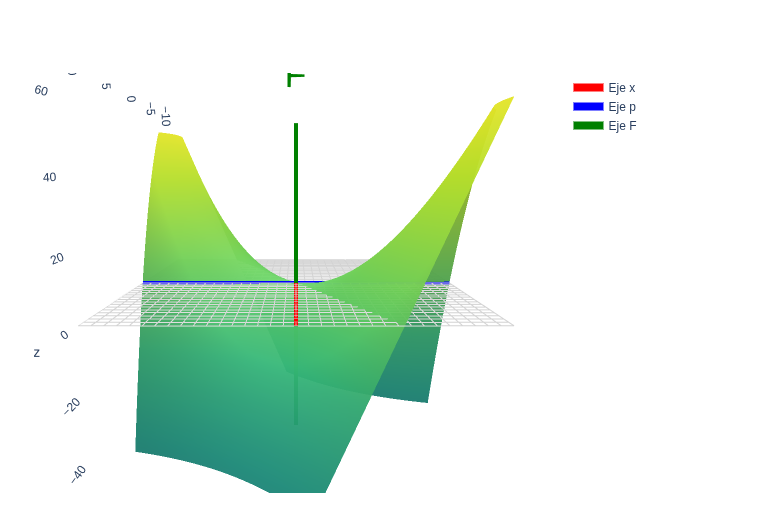
\includegraphics[width=0.75\textwidth]{lateral.png}
\caption{Vista \textbf{lateral} donde se ve con mayor claridad cómo, para cada $p$ fijo, la sección en el plano $(x,F)$ es una parábola que abre hacia abajo}
\label{fig:Fxp_lateral}
\end{figure}

\begin{figure}[H]
\centering
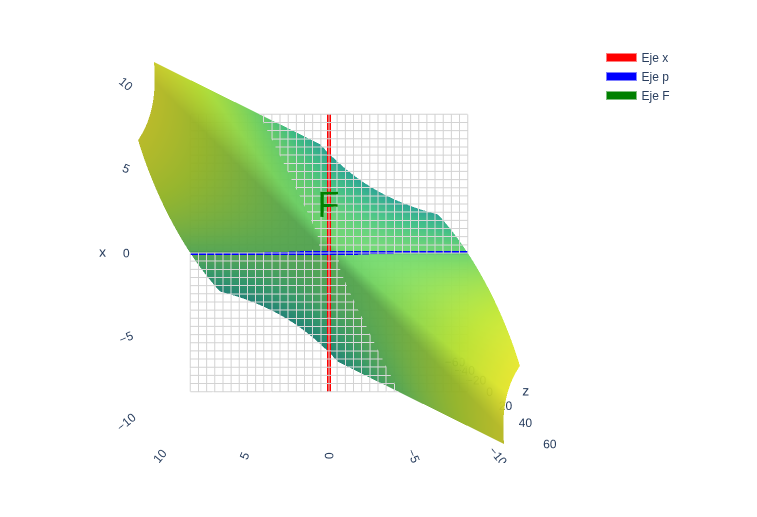
\includegraphics[width=0.75\textwidth]{superior.png}
\caption{Vista \textbf{superior} de la superficie, enfatizando el plano $(x,p)$ y la proyección de la gráfica sobre él}
\label{fig:Fxp_superior}
\end{figure}

En todas estas vistas se observan dos características esenciales de la función:

\begin{itemize}
  \item[$\bullet$] Para $p$ fijo, la expresión
  \[
    F(x,p) = -\,\frac{x^{2}}{2} + p\,x
  \]
  describe una \textbf{parábola} en el plano $(x,F)$, con apertura hacia abajo  
 \item[$\bullet$] Para $x$ fijo, la función es \textbf{lineal} en $p$,
  \[
    F(x,p) = x\,p - \text{(término que sólo depende de $x$)}
  \]
  de modo que, al movernos a lo largo del eje $p$, los puntos de la superficie se desplazan sobre rectas
\end{itemize}

Estos dos comportamientos —parabólico en $x$ y lineal en $p$— son la base de la forma “tipo valle–cresta” que se aprecia en las figuras \ref{fig:Fxp_frontal}–\ref{fig:Fxp_superior}.

\vspace{0.3cm}
\textcolor{trueblue}{\textbf{Derivadas parciales y curva de máximos sobre la superficie}}

Para entender mejor la estructura de la superficie, calculamos las derivadas parciales de $F$ con respecto a sus variables
\begin{equation}
\begin{split}
\frac{\partial F}{\partial x} &= p - x \\[4pt]
\frac{\partial F}{\partial p} &= x
\end{split}\label{eq:derivadas-F-cuadratica-again}
\end{equation}
La condición de extremo con respecto a $x$, manteniendo $p$ fijo, se obtiene imponiendo
\[
\frac{\partial F}{\partial x} = 0
\]
lo que conduce a
\begin{equation}
\begin{split}
p - x &= 0 \\[4pt]
\Rightarrow\quad x &= p
\end{split}\label{eq:recta-critica-cuadratica-again}
\end{equation}

Esta recta $x=p$ en el plano $(x,p)$ juega un papel central: sobre ella se encuentran, para cada $p$, los puntos donde $F(x,p)$ es extremo respecto a $x$.  
En el contexto de la transformada de Legendre, la relación
\[
p = \frac{d f(x)}{dx}
\]
corresponde precisamente a \eqref{eq:recta-critica-cuadratica-again}, ya que
\begin{equation}
\begin{split}
\frac{d f(x)}{dx} &= \frac{d}{dx} \left( \frac{x^{2}}{2} \right) = x
\end{split}\label{eq:f-prima-cuadratica-again}
\end{equation}

Si evaluamos de nuevo la función sobre esta recta crítica, sustituyendo $x=p$ en \eqref{eq:F-cuadratica-explicita-again}, obtenemos
\begin{equation}
\begin{split}
g(p) &= F(p,p) = p^{2} - \frac{p^{2}}{2} = \frac{p^{2}}{2}
\end{split}\label{eq:g-de-p-again}
\end{equation}
La función $g(p)$ es una parábola en el plano $(p,g)$ y representa el \emph{valor extremo} de $F(x,p)$ respecto a $x$ para cada $p$.  
Geométricamente, puede interpretarse como el “lomo” de la superficie: los vértices de las parábolas obtenidas al fijar $p$ se alinean precisamente sobre esta curva $g(p)$.

\begin{figure}[H]
\centering
  \begin{minipage}{0.45\textwidth}
    \centering
    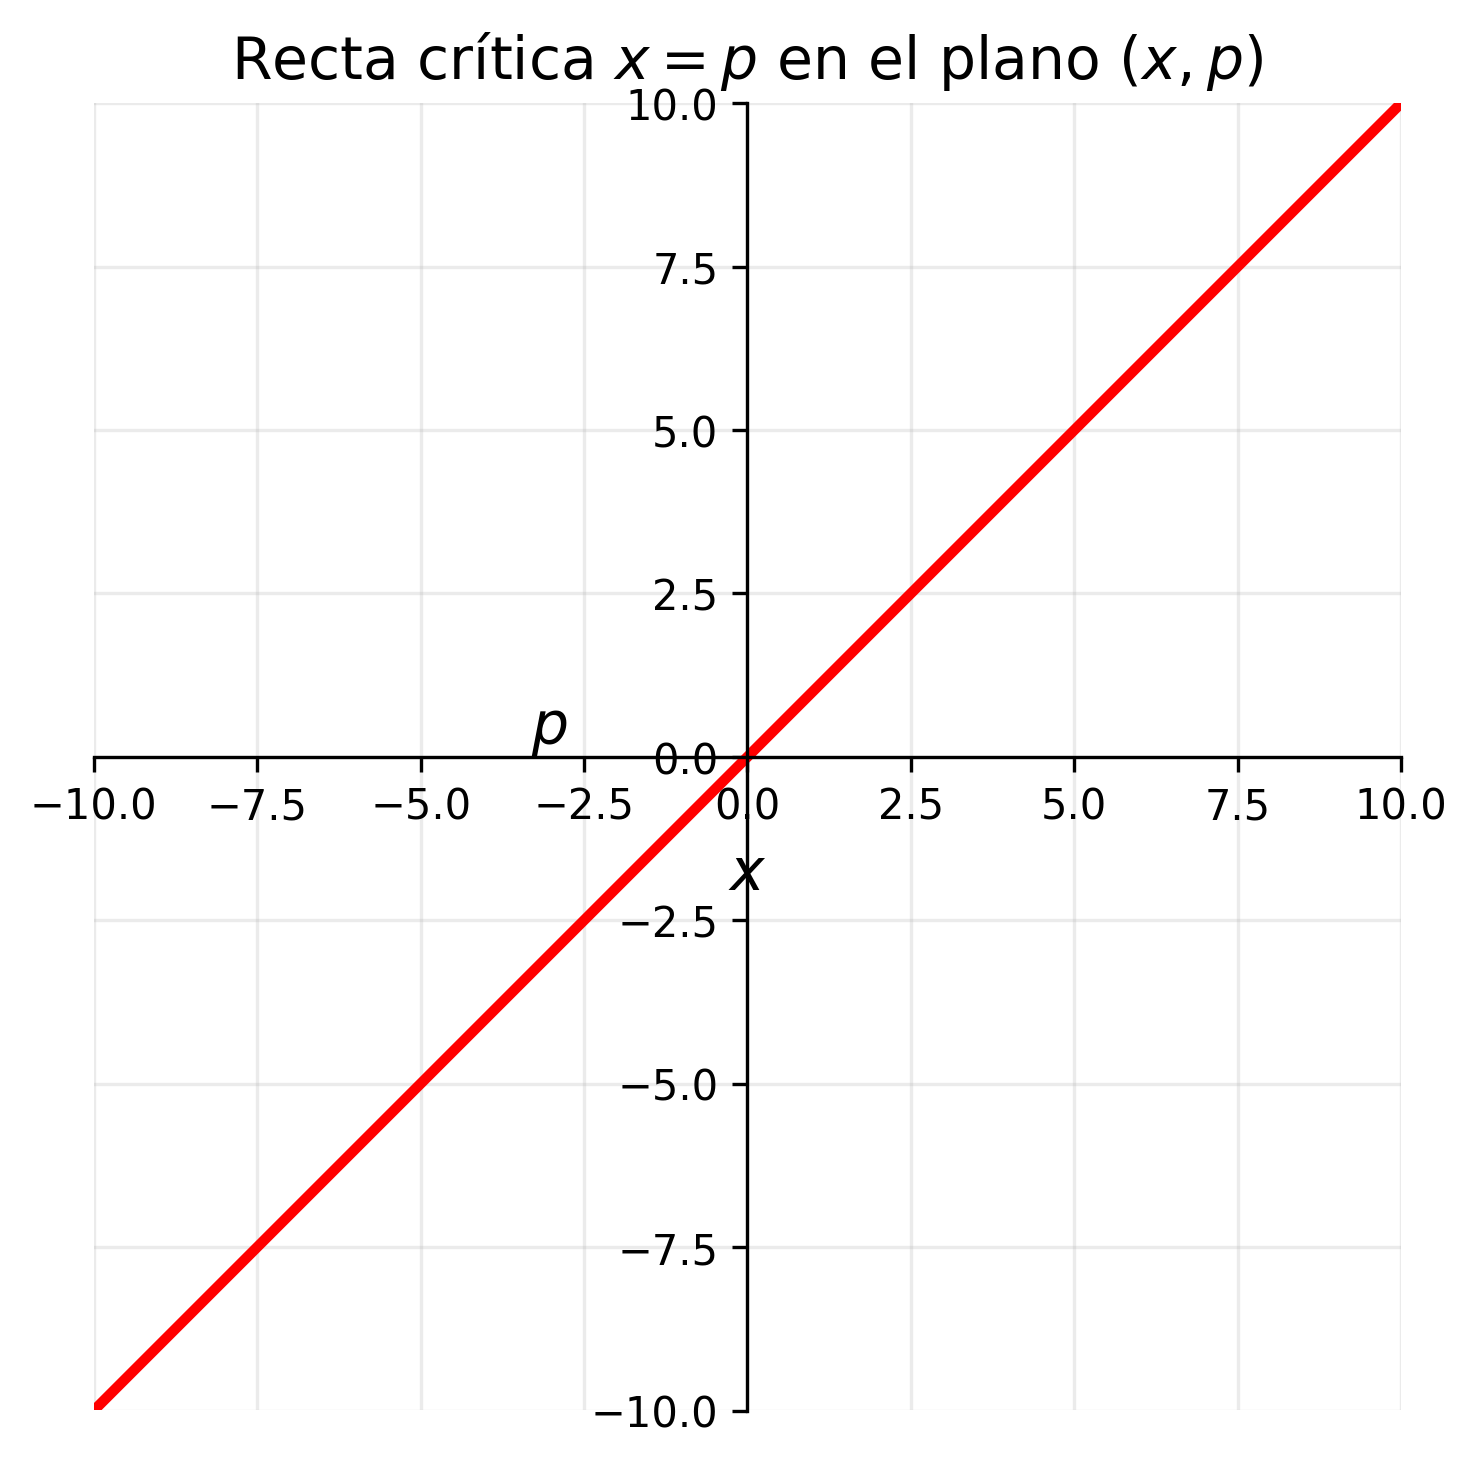
\includegraphics[width=\textwidth]{recta_x_igual_p.png}
    \caption{Recta crítica $x=p$ en el plano $(x,p)$}
    \label{fig:recta_critica}
  \end{minipage}\hfill
  \begin{minipage}{0.45\textwidth}
    \centering
    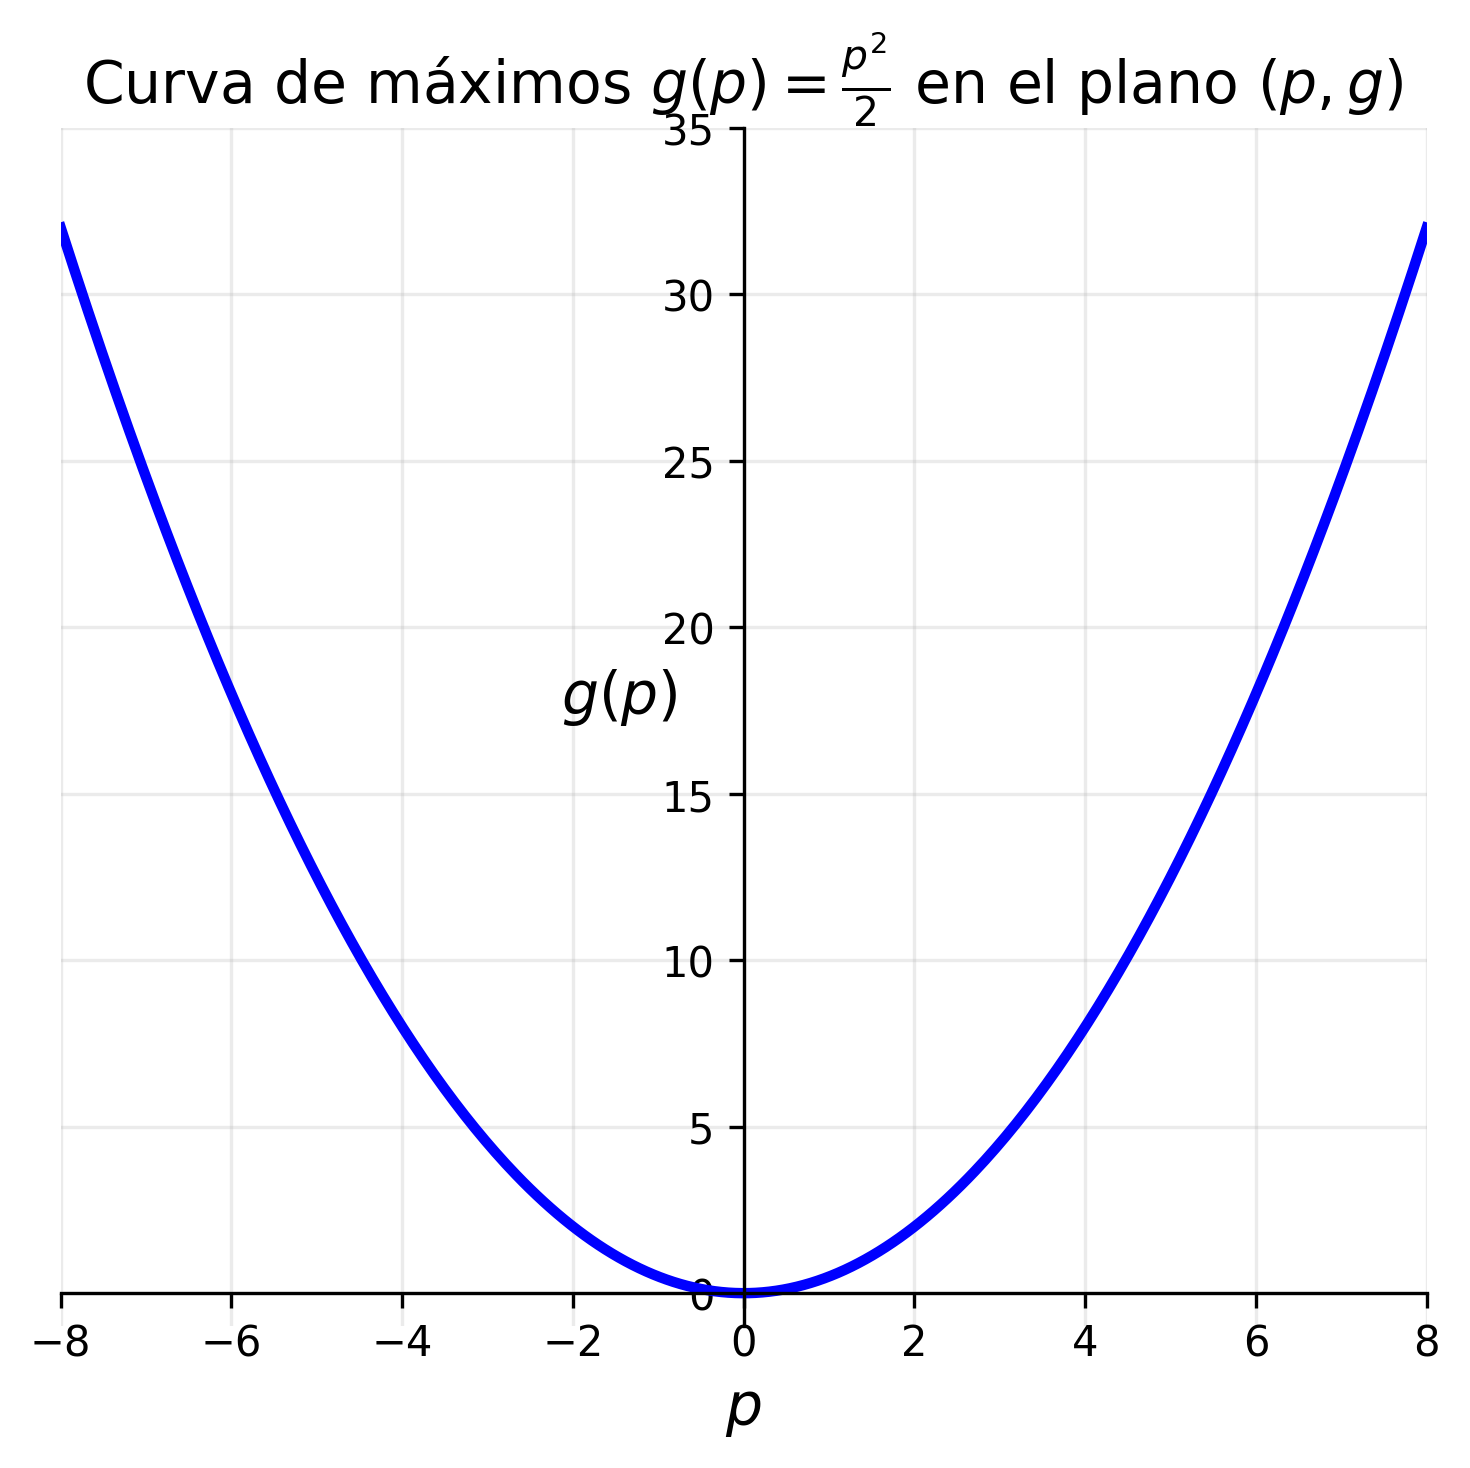
\includegraphics[width=\textwidth]{g_de_p_parabola.png}
    \caption{Curva de máximos $g(p)=\frac{p^{2}}{2}$ en el plano $(p,g)$}
    \label{fig:g_de_p}
  \end{minipage}
\end{figure}

\begin{figure}[H]
\centering
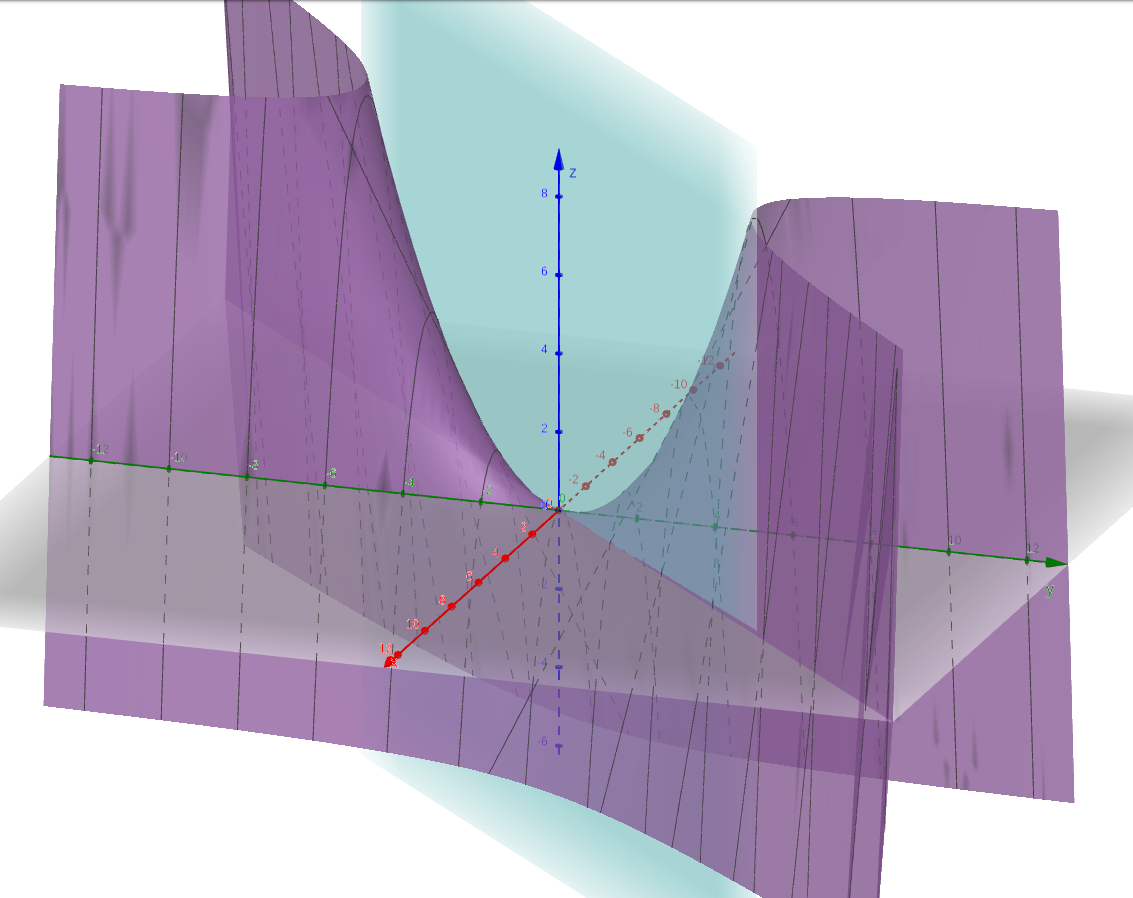
\includegraphics[width=0.75\textwidth]{Fxp_superficie_plano_recta_g.png}
\caption{Superficie $F(x,p) = p x - x^{2}/2$ mostrando el plano crítico $x=p$ y la curva de máximos $g(p)=p^{2}/2$ sobre dicho plano}
\label{fig:Fxp_plano_legendre}
\end{figure}

\vspace{0.4cm}

Así de esta manera la superficie tridimensional de $F(x,p)$ representada en las figuras 
\ref{fig:Fxp_frontal}–\ref{fig:Fxp_superior}, junto con las figuras 
\ref{fig:recta_critica} y \ref{fig:g_de_p}, puede entenderse como la combinación de tres estructuras geométricas fundamentales:

\begin{itemize}
  \item[$\bullet$] parábolas en la dirección de $x$ para cada valor fijo de $p$,
  \item[$\bullet$] rectas en la dirección de $p$ para cada valor fijo de $x$,
  \item[$\bullet$] y una curva de máximos $g(p)=p^{2}/2$ situada sobre la recta crítica $x=p$.
\end{itemize}

Esta organización geométrica surge directamente de la forma analítica de la función en 
\eqref{eq:F-cuadratica-explicita-again} y se conecta de manera natural con la teoría de la
transformada de Legendre discutida en el capítulo.

%-------------------- Parte (b): familia de funciones F_{p0}(x) cuadráticas --------------------

\vspace{0.5cm}
\textbf{(b) Familia de funciones $F_{p_{0}}(x)=p_{0}x - x^{2}/2$ para $p_{0}=-10,\dots,10$}

Fijemos ahora el parámetro \(p\) en un valor constante \(p_{0}\). De este modo, la función
original \(F(x,p)\) se convierte en una familia uniparamétrica de funciones de una sola
variable

\begin{equation}
\begin{split}
F_{p_{0}}(x) &\equiv p_{0}x - \frac{x^{2}}{2}
\end{split}\label{eq:Fp0-cuadratica}
\end{equation}

Cada miembro de esta familia es una \textbf{parábola que abre hacia abajo}, pues el
coeficiente del término cuadrático en \(x\) es negativo. La forma de la curva es siempre
la misma; lo que cambia, al variar \(p_{0}\), es su \textbf{posición horizontal} y la
\textbf{altura de su máximo}.

Para localizar el vértice de cada parábola derivamos respecto a \(x\)

\begin{equation}
\begin{split}
\frac{dF_{p_{0}}}{dx} &= p_{0} - x = 0 \\[4pt]
\Rightarrow\quad x_{\text{vértice}} &= p_{0}
\end{split}\label{eq:vertice-cuadratica}
\end{equation}

Sustituyendo este valor en \eqref{eq:Fp0-cuadratica} obtenemos la altura máxima

\begin{equation}
\begin{split}
F_{p_{0}}(p_{0})
&= p_{0}^{2} - \frac{p_{0}^{2}}{2} \\[4pt]
&= \frac{p_{0}^{2}}{2}
\end{split}\label{eq:maximo-cuadratica}
\end{equation}

Esta expresión coincide con la obtenida previamente al analizar la superficie
\(F(x,p)\). La razón es que la condición de máximo
\[
\frac{\partial F}{\partial x} = 0
\]
es idéntica a la condición que aparece en la construcción de la
\textcolor{trueblue}{\textbf{transformada de Legendre}}. En este caso particular, el
punto extremo está dado simplemente por
\[
x(p_{0}) = p_{0},
\qquad
F_{\text{ext}}(p_{0}) = \frac{p_{0}^{2}}{2}
\]

Así, cada valor de \(p_{0}\) determina:

\begin{itemize}
  \item[$\bullet$] la posición del vértice de la parábola, que siempre queda en \(x=p_{0}\)
  \item[$\bullet$] la altura máxima de la curva, igual a \(\dfrac{p_{0}^{2}}{2}\)
  \item[$\bullet$] una parábola que conserva exactamente la misma forma pero aparece centrada en un valor distinto de \(x\)
\end{itemize}


Al considerar el conjunto completo
\[
p_{0}\in\{-10,-9,\dots,-1,0,1,\dots,9,10\}
\]
obtenemos \(21\) parábolas, todas con la misma “curvatura” (el coeficiente de \(x^{2}\)
es siempre \(-1/2\)), pero con vértices situados en diferentes puntos \(x=p_{0}\) y con
distintas alturas máximas \(\dfrac{p_{0}^{2}}{2}\).

Estas curvas pueden representarse en una sola figura en el plano \((x,F)\). A
continuación se muestra un ejemplo de código en \texttt{pgfplots} que genera dicha
familia de funciones, destacando con mayor grosor los casos \(p_{0}=-10\), \(p_{0}=0\)
y \(p_{0}=10\)

\begin{center}
\begin{tikzpicture}
\begin{axis}[
    xlabel={$x$},
    ylabel={$F_{p_{0}}(x) = p_{0}x - \dfrac{x^{2}}{2}$},
    xmin=-11, xmax=11,
    ymin=-200, ymax=80,
    axis lines=middle,
    grid=both,
    width=20cm,
    height=18cm,
    legend style={
        font=\footnotesize,
        at={(0.02,0.02)},
        anchor=south west
    },
    legend cell align=left,
    domain=-11:11,
    samples=200
]

  %--- 21 parábolas, p0 = -10,...,10, cada una con color explícito ---

  % p0 = -10
  \addplot[thin, color=Cinnabar] {-10*x - x^2/2};

  % p0 = -9
  \addplot[thin, color=trueblue] {-9*x - x^2/2};

  % p0 = -8
  \addplot[thin, color=Lochmara] {-8*x - x^2/2};

  % p0 = -7
  \addplot[thin, color=Horizon] {-7*x - x^2/2};

  % p0 = -6
  \addplot[thin, color=Hippie Blue] {-6*x - x^2/2};

  % p0 = -5
  \addplot[thin, color=Victoria] {-5*x - x^2/2};

  % p0 = -4
  \addplot[thin, color=Logan] {-4*x - x^2/2};

  % p0 = -3
  \addplot[thin, color=Apple Green] {-3*x - x^2/2};

  % p0 = -2
  \addplot[thin, color=Android Green] {-2*x - x^2/2};

  % p0 = -1
  \addplot[thin, color=Viridian Green] {-1*x - x^2/2};

  % p0 = 0
  \addplot[thin, color=tealgreen] {-x^2/2};

  % p0 = 1
  \addplot[thin, color=Bluechill] {1*x - x^2/2};

  % p0 = 2
  \addplot[thin, color=brightturquoise] {2*x - x^2/2};

  % p0 = 3
  \addplot[thin, color=Sun] {3*x - x^2/2};

  % p0 = 4
  \addplot[thin, color=Saffron] {4*x - x^2/2};

  % p0 = 5
  \addplot[thin, color=orange(colorwheel)] {5*x - x^2/2};

  % p0 = 6
  \addplot[thin, color=Mahogany] {6*x - x^2/2};

  % p0 = 7
  \addplot[thin, color=Electric Violet] {7*x - x^2/2};

  % p0 = 8
  \addplot[thin, color=darkviolet] {8*x - x^2/2};

  % p0 = 9
  \addplot[thin, color=wisteria] {9*x - x^2/2};

  % p0 = 10
  \addplot[thin, color=Apple Green] {10*x - x^2/2};

  %--- Volvemos a dibujar p0=-10,0,10 más gruesas sobre todo ---
  \addplot[very thick, color=Cinnabar] {-10*x - x^2/2};
  \addplot[very thick, color=trueblue] {-x^2/2};
  \addplot[very thick, color=AppleGreen] {10*x - x^2/2};

  %--- LEYENDA: forzamos estilo de línea y color de texto ---
  \addlegendimage{no markers, very thick, color=Cinnabar}
  \addlegendentry{\textcolor{Cinnabar}{$p_{0}=-10$}}

  \addlegendimage{no markers, very thick, color=trueblue}
  \addlegendentry{\textcolor{trueblue}{$p_{0}=0$}}

  \addlegendimage{no markers, very thick, color=AppleGreen}
  \addlegendentry{\textcolor{AppleGreen}{$p_{0}=10$}}

\end{axis}
\end{tikzpicture}
\end{center}



Esta figura muestra claramente cómo se “desplaza” el vértice de cada parábola a lo
largo del eje \(x\) conforme cambia el parámetro \(p_{0}\). El papel de \(p_{0}\) es
seleccionar, dentro de la superficie tridimensional \(F(x,p)\), una sección vertical
fija y, dentro de esa sección, el punto que hace extrema la función de acuerdo con la
receta de Legendre.

%-------------------- Repetir el análisis para F(x,p) = px - x^{3}/3 --------------------

\vspace{0.6cm}
\textbf{Análisis para $F(x,p) = px - x^{3}/3$}

Consideremos ahora la función
\begin{equation}
\begin{split}
F(x,p) &= p\,x - \frac{x^{3}}{3}
\end{split}\label{eq:F-cubica}
\end{equation}

De nuevo, se reconoce la estructura general
\[
F(x,p) = p\,x - f(x)
\]
pero ahora la función de una variable \(x\) está dada por
\begin{equation}
\begin{split}
f(x) &= \frac{x^{3}}{3}
\end{split}\label{eq:f-cubica}
\end{equation}

%-------------------- Parte (a): gráfica 3D de F(x,p) cúbica --------------------

\vspace{0.3cm}
\textbf{(a) Gráfica en tres dimensiones de $F(x,p) = px - x^{3}/3$}

Como en el caso anterior, pensamos en \(F\) como una función
\[
F:\mathbb{R}^{2}\longrightarrow\mathbb{R},
\qquad (x,p)\longmapsto F(x,p)
\]
cuya gráfica es una superficie en el espacio tridimensional con coordenadas \((x,p,F)\).
Para estudiar su forma, calculamos las derivadas parciales
\begin{equation}
\begin{split}
\frac{\partial F}{\partial x} &= p - x^{2} \\[4pt]
\frac{\partial F}{\partial p} &= x
\end{split}\label{eq:derivadas-F-cubica}
\end{equation}

La condición de extremo respecto a \(x\), manteniendo fijo \(p\), se escribe como
\[
\frac{\partial F}{\partial x} = 0
\]
lo cual conduce a
\begin{equation}
\begin{split}
p - x^{2} &= 0 \\[4pt]
\Rightarrow\quad p &= x^{2}
\end{split}\label{eq:parabola-critica-cubica}
\end{equation}

Si derivamos la función \(f(x)\) en \eqref{eq:f-cubica}, obtenemos
\begin{equation}
\begin{split}
f'(x) &= \frac{d}{dx}\left(\frac{x^{3}}{3}\right) = x^{2}
\end{split}\label{eq:f-prima-cubica}
\end{equation}
de modo que la condición de extremo \eqref{eq:parabola-critica-cubica} puede
reescribirse como
\[
p = f'(x)
\]
que es exactamente la ecuación que aparece en la construcción de la
\textcolor{trueblue}{\textbf{transformada de Legendre}}

Si ahora queremos escribir \(x\) como función de la nueva variable \(p\), resolvemos
\eqref{eq:parabola-critica-cubica} para \(x\)
\begin{equation}
\begin{split}
p &= x^{2} \\[4pt]
\Rightarrow\quad x &= x_{\pm}(p) = \pm\sqrt{p}, \qquad p \ge 0
\end{split}\label{eq:x-mas-menos-raizp}
\end{equation}

Es decir, para cada valor de \(p\ge 0\) existen dos soluciones posibles para \(x\),
de modo que en este ejemplo la transformada de Legendre tendrá dos ramas.
Evaluando \(F(x,p)\) en cada una de estas soluciones \(x_{\pm}(p)\) obtenemos
\begin{equation}
\begin{split}
g_{\pm}(p)
&= F\bigl(x_{\pm}(p),p\bigr) \\[4pt]
&= p\bigl(\pm\sqrt{p}\bigr) - \frac{\bigl(\pm\sqrt{p}\bigr)^{3}}{3} \\[4pt]
&= \pm p^{3/2} \mp \frac{p^{3/2}}{3} \\[4pt]
&= \pm \frac{2}{3}\,p^{3/2}
\end{split}\label{eq:g-mas-menos}
\end{equation}

Por lo tanto, para este ejemplo la transformada de Legendre asociada a
\(f(x)=x^{3}/3\) queda descrita por las dos ramas
\[
g_{+}(p) = \frac{2}{3}p^{3/2},
\qquad
g_{-}(p) = -\,\frac{2}{3}p^{3/2},
\qquad p \ge 0
\]

La curva de puntos extremos de la superficie en el espacio \((x,p,F)\) se puede
escribir, de manera equivalente, en forma paramétrica
\[
(x,p,F) = \left(x,\,x^{2},\,\frac{2}{3}x^{3}\right)
\]
tomando \(x\) como parámetro, o bien
\[
(x,p,F) = \bigl(x_{\pm}(p),\,p,\,g_{\pm}(p)\bigr)
\]
tomando \(p\) como parámetro y distinguiendo las dos ramas \(x_{\pm}(p)\)

La superficie \(F(x,p)=px-x^{3}/3\) se representó en un sistema de coordenadas
tridimensional \((x,p,F)\) utilizando \texttt{GeoGebra}.  
En las siguientes figuras se muestran tres vistas complementarias de la misma
superficie.

\begin{figure}[H]
\centering
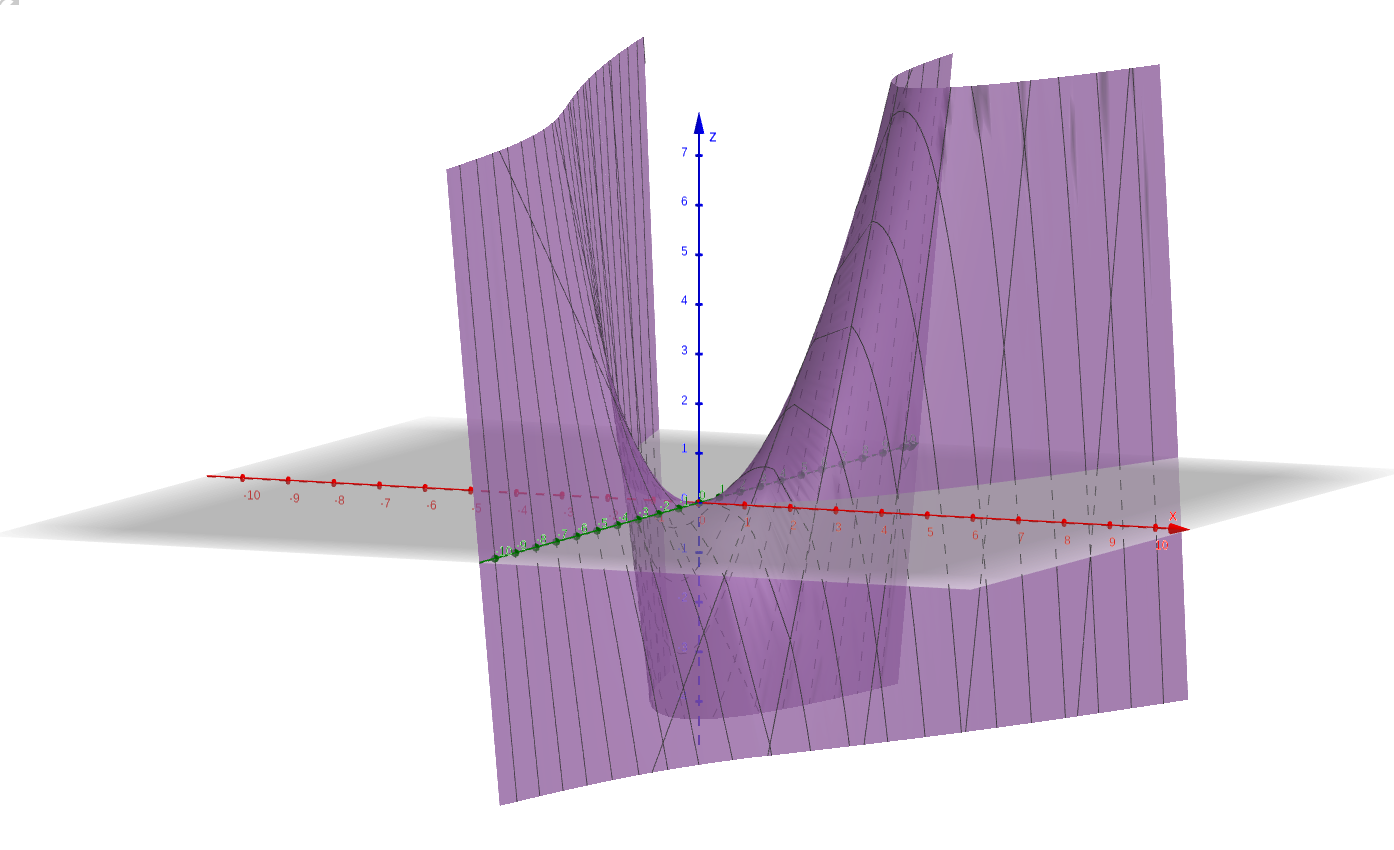
\includegraphics[width=0.9\textwidth]{ultima_gráfica.png}
\caption{Vista general de la superficie $F(x,p)=px-x^{3}/3$ obtenida con \texttt{GeoGebra}. Se observa el plano $F=0$ (gris) y los ejes coordenados, destacando la dependencia cúbica en $x$ y lineal en $p$}
\label{fig:Fxp_cubica_geo_1}
\end{figure}

\begin{figure}[H]
\centering
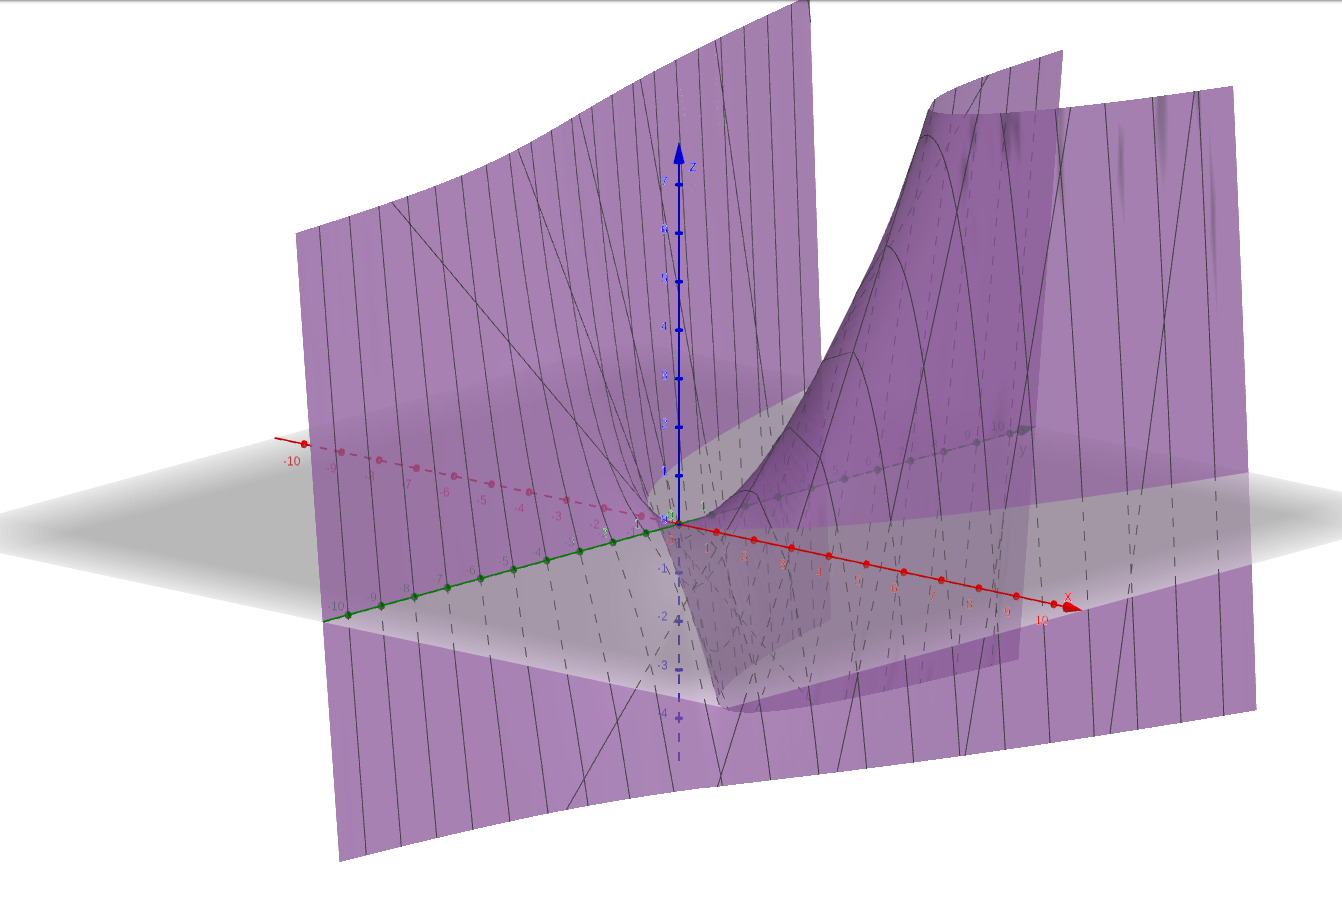
\includegraphics[width=0.9\textwidth]{ultima_gráfica_2.png}
\caption{Vista oblicua donde se aprecia con mayor claridad la parábola crítica $p=x^{2}$ sobre el plano $(x,p)$ y la región cercana al origen donde se concentran los puntos extremos de la superficie}
\label{fig:Fxp_cubica_geo_2}
\end{figure}

\begin{figure}[H]
\centering
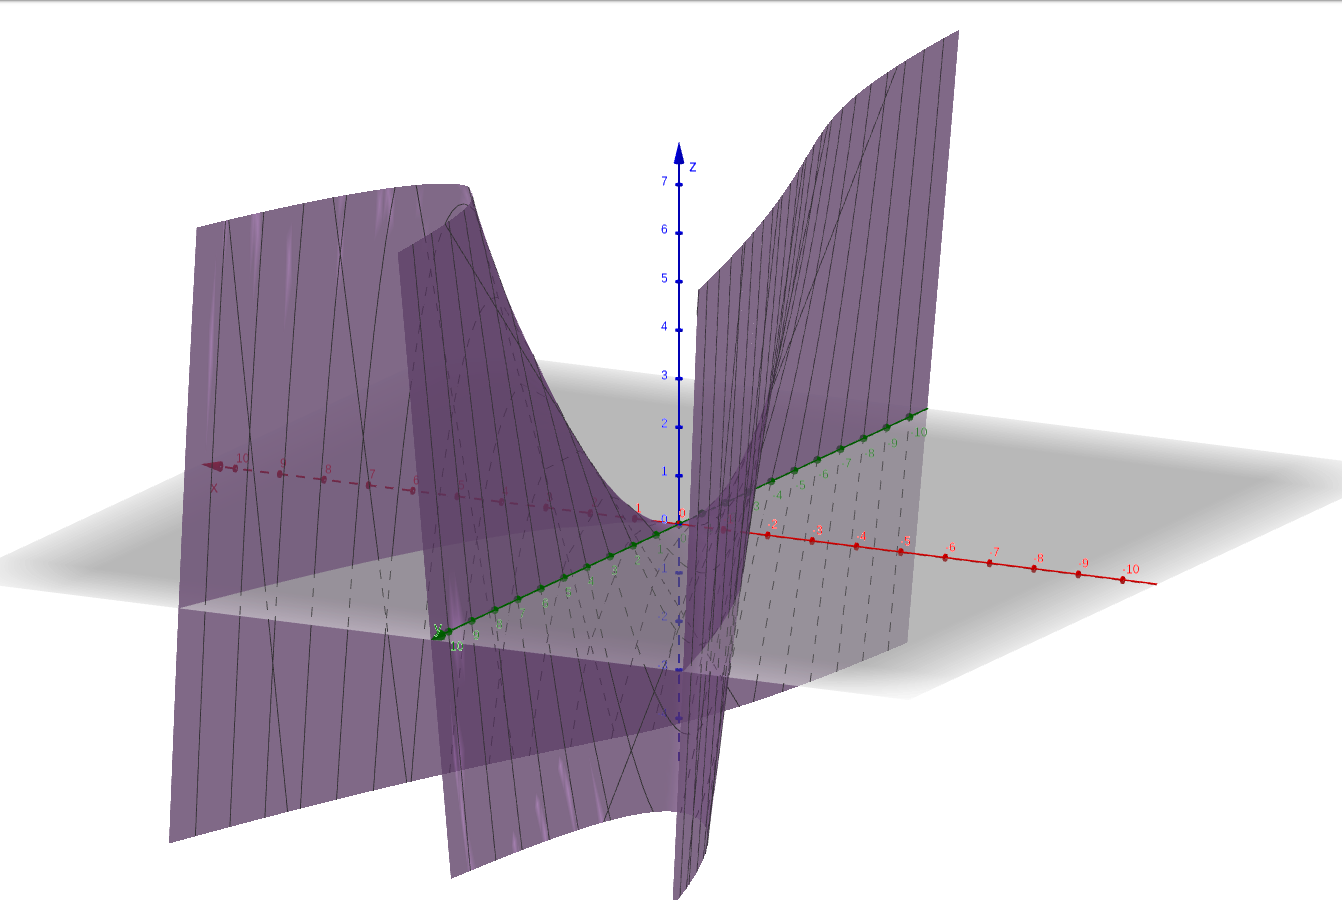
\includegraphics[width=0.9\textwidth]{útima_gráfica_3.png}
\caption{Vista lateral de la superficie mostrando las secciones verticales $p=p_{0}$ como curvas cúbicas $F_{p_{0}}(x)=p_{0}x-x^{3}/3$; para $p_{0}>0$ se distinguen los máximos y mínimos locales asociados a la condición $\partial F/\partial x=0$}
\label{fig:Fxp_cubica_geo_3}
\end{figure}

Estas gráficas muestran una superficie cuya dependencia en \(x\) es cúbica y cuya
dependencia en \(p\) sigue siendo lineal, lo que produce una forma más “torcida” que
en el caso cuadrático, pero que obedece a la misma regla de puntos críticos
\(\partial F/\partial x = 0\) asociada a la transformada de Legendre


%-------------------- Parte (b): familia de funciones F_{p0}(x) cúbicas --------------------

\vspace{0.5cm}
\textbf{(b) Familia de funciones $F_{p_{0}}(x)=p_{0}x - x^{3}/3$ para $p_{0}=-10,\dots,10$}

Al igual que antes, fijamos ahora el parámetro \(p\) en un valor constante \(p_{0}\) y
definimos
\begin{equation}
\begin{split}
F_{p_{0}}(x) &\equiv p_{0}x - \frac{x^{3}}{3}
\end{split}\label{eq:Fp0-cubica}
\end{equation}

Cada función \(F_{p_{0}}(x)\) es ahora una \textbf{curva cúbica} en el plano \((x,F)\).
Para entender su forma cualitativa derivamos respecto a \(x\)
\begin{equation}
\begin{split}
\frac{dF_{p_{0}}}{dx} &= p_{0} - x^{2}
\end{split}\label{eq:derivada-Fp0-cubica}
\end{equation}
y analizamos los puntos críticos que satisfacen
\begin{equation}
\begin{split}
p_{0} - x^{2} &= 0 \\[4pt]
\Rightarrow\quad x &= \pm\sqrt{p_{0}}
\end{split}\label{eq:criticos-cubica}
\end{equation}

De aquí se desprende que

\begin{itemize}
  \item si \(p_{0} > 0\), la función \(F_{p_{0}}(x)\) tiene dos puntos críticos reales
  en \(x = \pm\sqrt{p_{0}}\); uno corresponde a un máximo local y el otro a un mínimo local
  \item si \(p_{0} = 0\), la función se reduce a
  \[
    F_{0}(x) = -\,\frac{x^{3}}{3}
  \]
  que presenta un punto de inflexión en \(x=0\), pero no máximos ni mínimos locales
  \item si \(p_{0} < 0\), la ecuación \(p_{0} - x^{2} = 0\) no tiene soluciones reales, de modo
  que \(F_{p_{0}}(x)\) no presenta extremos locales reales y su gráfica es monótona,
  con la curvatura típica de una función cúbica
\end{itemize}

En todos los casos, el comportamiento asintótico está dominado por el término cúbico
\(-x^{3}/3\), de modo que
\[
\lim_{x\to +\infty} F_{p_{0}}(x) = -\infty,
\qquad
\lim_{x\to -\infty} F_{p_{0}}(x) = +\infty
\]
lo cual es característico de las funciones cúbicas con coeficiente negativo en el
término de mayor grado

Podemos representar en un solo gráfico la familia de curvas
\(\{F_{p_{0}}(x)\}_{p_{0}=-10}^{10}\). Un código típico en \texttt{pgfplots} es
\begin{center}
\begin{tikzpicture}
\begin{axis}[
    xlabel={$x$},
    ylabel={$F_{p_{0}}(x) = p_{0}x - \dfrac{x^{3}}{3}$},
    xmin=-4, xmax=4,
    ymin=-80, ymax=80,
    axis lines=middle,
    grid=both,
    width=20cm,
    height=18cm,
    legend style={
        font=\footnotesize,
        at={(0.02,0.02)},
        anchor=south west
    },
    legend cell align=left,
    domain=-4:4,
    samples=400
]

  %--- Familia de curvas cúbicas, p0 = -10,...,10 ---

  % p0 = -10
  \addplot[thin, color=Cinnabar] {-10*x - x^3/3};

  % p0 = -9
  \addplot[thin, color=trueblue] {-9*x - x^3/3};

  % p0 = -8
  \addplot[thin, color=Lochmara] {-8*x - x^3/3};

  % p0 = -7
  \addplot[thin, color=Horizon] {-7*x - x^3/3};

  % p0 = -6
  \addplot[thin, color=Hippie Blue] {-6*x - x^3/3};

  % p0 = -5
  \addplot[thin, color=Victoria] {-5*x - x^3/3};

  % p0 = -4
  \addplot[thin, color=Logan] {-4*x - x^3/3};

  % p0 = -3
  \addplot[thin, color=Apple Green] {-3*x - x^3/3};

  % p0 = -2
  \addplot[thin, color=Android Green] {-2*x - x^3/3};

  % p0 = -1
  \addplot[thin, color=Viridian Green] {-1*x - x^3/3};

  % p0 = 0
  \addplot[thin, color=tealgreen] {-x^3/3};

  % p0 = 1
  \addplot[thin, color=Bluechill] {1*x - x^3/3};

  % p0 = 2
  \addplot[thin, color=brightturquoise] {2*x - x^3/3};

  % p0 = 3
  \addplot[thin, color=Sun] {3*x - x^3/3};

  % p0 = 4
  \addplot[thin, color=Saffron] {4*x - x^3/3};

  % p0 = 5
  \addplot[thin, color=orange(colorwheel)] {5*x - x^3/3};

  % p0 = 6
  \addplot[thin, color=Mahogany] {6*x - x^3/3};

  % p0 = 7
  \addplot[thin, color=Electric Violet] {7*x - x^3/3};

  % p0 = 8
  \addplot[thin, color=darkviolet] {8*x - x^3/3};

  % p0 = 9
  \addplot[thin, color=wisteria] {9*x - x^3/3};

  % p0 = 10
  \addplot[thin, color=Apple Green] {10*x - x^3/3};

\end{axis}
\end{tikzpicture}
\end{center}

En esta figura se aprecia cómo, al variar \(p_{0}\), cambian la inclinación y la forma
local de la curva cúbica \(F_{p_{0}}(x)\). Para \(p_{0}>0\) aparecen máximos y mínimos
locales en \(x=\pm\sqrt{p_{0}}\), mientras que para \(p_{0}\leq 0\) desaparecen los
extremos reales y la curva se vuelve monótona. Una vez más, la condición
\(p_{0}=f'(x)\) conecta de manera directa este comportamiento con la receta general de
la transformada de Legendre discutida en el capítulo

%=============================
% PR. 4.2
%=============================

\begin{AGbox}[8]
\begin{enumerate}[label={{\textcolor{trueblue}{\textbf{Pr.} 4.2}}}]
  \item Para una partícula libre, en una dimensión, en un solo gráfico, presente las trayectorias correspondientes a diferentes condiciones iniciales, en el espacio fase con coordenadas $(x,p)$, y en el espacio fase extendido con coordenadas $(x,p,t)$. Ademàs, presentar las gráficas correspondientes para el oscilador armónico simple.
\end{enumerate}
\end{AGbox}
\vspace{0.5cm}

\textcolor{Cinnabar}{\textbf{Solución:}} \vspace{0.5cm}

En este problema se nos pide representar las trayectorias de dos sistemas mecánicos
muy importantes: la \textbf{partícula libre en una dimensión} y el \textbf{oscilador
armónico simple}.  
En ambos casos, la descripción se hace en el marco Hamiltoniano introducido en
el \textbf{Capítulo IV}, donde a cada sistema se le asocia una Hamiltoniana $H(x,p,t)$
y un sistema de ecuaciones de Hamilton para $(x(t),p(t))$

\begin{equation}
\begin{split}
\dot{x} &= \frac{\partial H}{\partial p} \\
\dot{p} &= -\,\frac{\partial H}{\partial x}
\end{split}
\label{eq:hamilton-ecuaciones-generales}
\end{equation}

Una vez obtenidas las soluciones $x(t)$ y $p(t)$, dichas soluciones definen:

\begin{itemize}
  \item[$\bullet$] trayectorias en el \textbf{espacio fase} $(x,p)$
  \item[$\bullet$] trayectorias en el \textbf{espacio fase extendido} $(x,p,t)$
\end{itemize}

A continuación analizamos por separado cada sistema.

%-------------------- 1) Partícula libre en una dimensión --------------------

\vspace{0.4cm}
\textbf{1) Partícula libre en una dimensión}

En el capítulo se estudia primero el caso de una partícula libre unidimensional con
Lagrangiana

\begin{equation}
\begin{split}
L(x,\dot{x},t) &= \frac{m}{2}\,\dot{x}^{2} \equiv T
\end{split}
\label{eq:L-libre-1D}
\end{equation}

Para construir la Hamiltoniana aplicamos la \textcolor{trueblue}{\textbf{transformación de Legendre}}.
Introducimos la función auxiliar

\begin{equation}
\begin{split}
F(x,\dot{x},t,p) &\equiv p\,\dot{x} - L(x,\dot{x},t)
\end{split}
\label{eq:F-legendre-libre}
\end{equation}

que en este caso toma la forma explícita

\begin{equation}
\begin{split}
F(x,\dot{x},t,p)
&= p\,\dot{x} - \frac{m}{2}\,\dot{x}^{2}
\end{split}
\label{eq:F-legendre-libre-explicita}
\end{equation}

La condición de extremo respecto a $\dot{x}$ se obtiene de

\[
\frac{\partial F}{\partial \dot{x}} = 0
\]

Usando \eqref{eq:F-legendre-libre-explicita}:

\begin{equation}
\begin{split}
\frac{\partial F}{\partial \dot{x}} &= p - m\,\dot{x} = 0
\end{split}
\label{eq:derivada-F-libre}
\end{equation}

de donde se obtiene la relación entre el momento y la velocidad

\begin{equation}
\begin{split}
p &= m\,\dot{x}
\end{split}
\label{eq:p-m-dotx}
\end{equation}

Resolviendo para $\dot{x}$:

\begin{equation}
\begin{split}
\dot{x} &= \frac{p}{m}
\end{split}
\label{eq:dotx-en-funcion-de-p}
\end{equation}

Con este resultado, la Hamiltoniana se define como

\begin{equation}
\begin{split}
H(x,p,t)
&\equiv F\bigl(x,\dot{x}(x,p,t),t,p\bigr) \\
&= p\,\dot{x}(x,p,t) - L\bigl(x,\dot{x}(x,p,t),t\bigr)
\end{split}
\label{eq:H-def-libre}
\end{equation}

Sustituyendo \eqref{eq:dotx-en-funcion-de-p} y \eqref{eq:L-libre-1D}:

\begin{equation}
\begin{split}
H(x,p,t)
&= p\left(\frac{p}{m}\right)
 - \frac{m}{2}\left(\frac{p}{m}\right)^{2} \\[4pt]
&= \frac{p^{2}}{m} - \frac{1}{2m}\,p^{2} \\[4pt]
&= \frac{p^{2}}{2m}
\end{split}
\label{eq:H-libre-final}
\end{equation}

Así, la transformación de Legendre conduce a

\begin{equation}
\begin{split}
H(x,p,t) &= \frac{p^{2}}{2m}
\end{split}
\label{eq:H-libre}
\end{equation}

Las ecuaciones de Hamilton son entonces

\begin{equation}
\begin{split}
\dot{x} &= \frac{\partial H}{\partial p} =  \frac{p}{m} \\[4pt]
\dot{p} &= -\frac{\partial H}{\partial x} = 0
\end{split}
\label{eq:hamilton-libre}
\end{equation}

La segunda ecuación implica que el momento es constante en el tiempo.


\begin{equation}
\begin{split}
p(t) &= p_{0} = cte
\end{split}
\end{equation}

donde $p_{0}$ es el valor inicial del momento al tiempo $t=0$.  
Sustituyendo este resultado en la ecuación para $\dot{x}$, se obtiene una ecuación
diferencial muy simple

\begin{equation}
\begin{split}
\dot{x}(t) &= \frac{p_{0}}{m}
\end{split}
\end{equation}

cuyas soluciones son rectas en el tiempo

\begin{equation}
\begin{split}
x(t) &= x_{0} + \frac{p_{0}}{m}\,t
\end{split}
\end{equation}

donde $x_{0}$ es la posición inicial al tiempo $t=0$.  
Por lo tanto, las trayectorias de una partícula libre en una dimensión, en la
formulación Hamiltoniana, están dadas por

\begin{equation}
\begin{split}
x(t) &= x_{0} + \frac{p_{0}}{m}\,t \\
p(t) &= p_{0}
\end{split}
\end{equation}

\vspace{0.3cm}
\textcolor{trueblue}{\textbf{Trayectorias en el espacio fase $(x,p)$}}

En el plano $(x,p)$ el tiempo $t$ no aparece explícitamente como coordenada, sino
como un \emph{parámetro} que recorre la solución $(x(t),p(t))$.  
Es decir, la trayectoria en espacio fase no es una gráfica de $p$ como función de $x$
ni de $x$ como función de $t$, sino la curva que describen simultáneamente
$x(t)$ y $p(t)$ conforme avanza el tiempo.

En el caso de la partícula libre, ya vimos que el momento es constante:

\[
p(t) = p_{0}
\]

y la posición evoluciona linealmente en el tiempo:

\[
x(t) = x_{0} + \frac{p_{0}}{m}t
\]

Por lo tanto, al eliminar el parámetro $t$ en la pareja $(x(t),p(t))$, obtenemos la
relación geométrica

\[
p = p_{0}
\]

lo que significa que la trayectoria en el espacio fase es una \textbf{recta horizontal}
a la altura $p_{0}$.  
Esta recta horizontal no describe “cómo cambia $p$ con $x$”, sino que representa que
\emph{mientras el tiempo avanza}, el punto $(x(t),p(t))$ se mueve únicamente en la
dirección del eje $x$, pues la coordenada $p$ permanece fija.

Desde un punto de vista geométrico:

\begin{itemize}
  \item[$\bullet$] la pendiente de la curva en el plano $(x,p)$ es
  \[
    \frac{dp}{dx} = 0
  \]
  porque $p$ no depende de $x$;
  
  \item[$\bullet$] el punto se traslada hacia la derecha si $p_{0}>0$, o hacia la izquierda
  si $p_{0}<0$, lo que refleja que la partícula libre mantiene una velocidad constante;

  \item[$\bullet$] cada una de estas rectas horizontales corresponde a un valor fijo de la
  energía cinética
  \[
    H = \frac{p_{0}^{2}}{2m},
  \]
  de modo que las líneas $p=\text{constante}$ son precisamente las curvas de nivel de la
  Hamiltoniana.
\end{itemize}

En consecuencia, la figura en el plano $(x,p)$ representa solamente la \emph{geometría}
de las trayectorias; el \emph{sentido del movimiento} y la rapidez con la que se recorre
cada recta horizontal están determinados por el parámetro $t$ (el cual no aparece en la
gráfica, pero sí en la solución paramétrica).

Un ejemplo de gráfico con varias trayectorias para distintos valores de $p_{0}$
puede producirse en \texttt{pgfplots} del siguiente modo:

\begin{center}
\begin{tikzpicture}
\begin{axis}[
    xlabel={$x$},
    ylabel={$p$},
    xmin=-5, xmax=5,
    ymin=-5, ymax=5,
    axis lines=middle,
    grid=both,
    width=12cm,
    height=8cm,
    legend style={
        font=\footnotesize,
        at={(0.02,0.98)},
        anchor=north west
    },
    legend cell align=left,
]

  % Tres valores de p0: -3, 0, 3
  \addplot[very thick, color=trueblue, domain=-5:5] {3};
  \addlegendentry{$p_{0}=3$}

  \addplot[very thick, color=Cinnabar, domain=-5:5] {0};
  \addlegendentry{$p_{0}=0$}

  \addplot[very thick, color=AppleGreen, domain=-5:5] {-3};
  \addlegendentry{$p_{0}=-3$}

\end{axis}
\end{tikzpicture}
\end{center}

En esta figura se muestran únicamente las curvas geométricas $p=\text{constante}$;
el movimiento sobre cada recta (hacia la derecha o hacia la izquierda) queda
implícito al hacer crecer el parámetro $t$.

\vspace{0.3cm}
\textcolor{trueblue}{\textbf{Trayectorias en el espacio fase extendido $(x,p,t)$}}

Al considerar el tiempo como tercera coordenada, el espacio fase extendido está
parametrizado por $(x,p,t)$.  
A partir de las soluciones obtenidas para la partícula libre, podemos escribir la
trayectoria completa en forma paramétrica como
\[
(x(t),p(t),t)
= \left(x_{0} + \frac{p_{0}}{m}t,\; p_{0},\; t\right)
\]

Esta expresión puede escribirse de manera equivalente como una recta en $\mathbb{R}^{3}$:
\[
\mathbf{r}(t) = \mathbf{r}_{0} + t\,\mathbf{v}
\]
donde
\[
\mathbf{r}_{0} = (x_{0},\,p_{0},\,0),
\qquad
\mathbf{v} = \left(\frac{p_{0}}{m},\,0,\,1\right)
\]

Lo cual muestra de manera inmediata que cada solución es una \textbf{recta}
en el espacio tridimensional $(x,p,t)$:

\begin{itemize}
  \item el punto inicial es $(x_{0},p_{0},0)$,
  \item la dirección de la recta está dada por el vector 
  \[
    \left(\frac{p_{0}}{m},\,0,\,1\right),
  \]
  \item la coordenada $p$ permanece constante e igual a $p_{0}$,
  \item la coordenada $x$ crece o decrece linealmente con $t$,
  \item el parámetro de la curva es precisamente el tiempo $t$.
\end{itemize}

Estas rectas pueden representarse directamente en \LaTeX\ usando el entorno
\texttt{tikzpicture} y la librería \texttt{pgfplots} en modo tridimensional.
Sin embargo, para reutilizar fácilmente la gráfica en otros documentos,
también es conveniente exportarla como imagen (\texttt{PNG}) a partir de un
archivo \texttt{standalone}.  

En la Figura~\ref{fig:trayectorias-xtp} se muestran las trayectorias
correspondientes a los valores
\[
p_{0} = -4,-3,-2,-1,0,1,2,3,4,
\]
tomando \(m=2\) y \(x_{0}=0\) en cada caso.

\begin{figure}[htbp]
  \centering
  % ajusta la ruta si tu PNG está en otra carpeta
  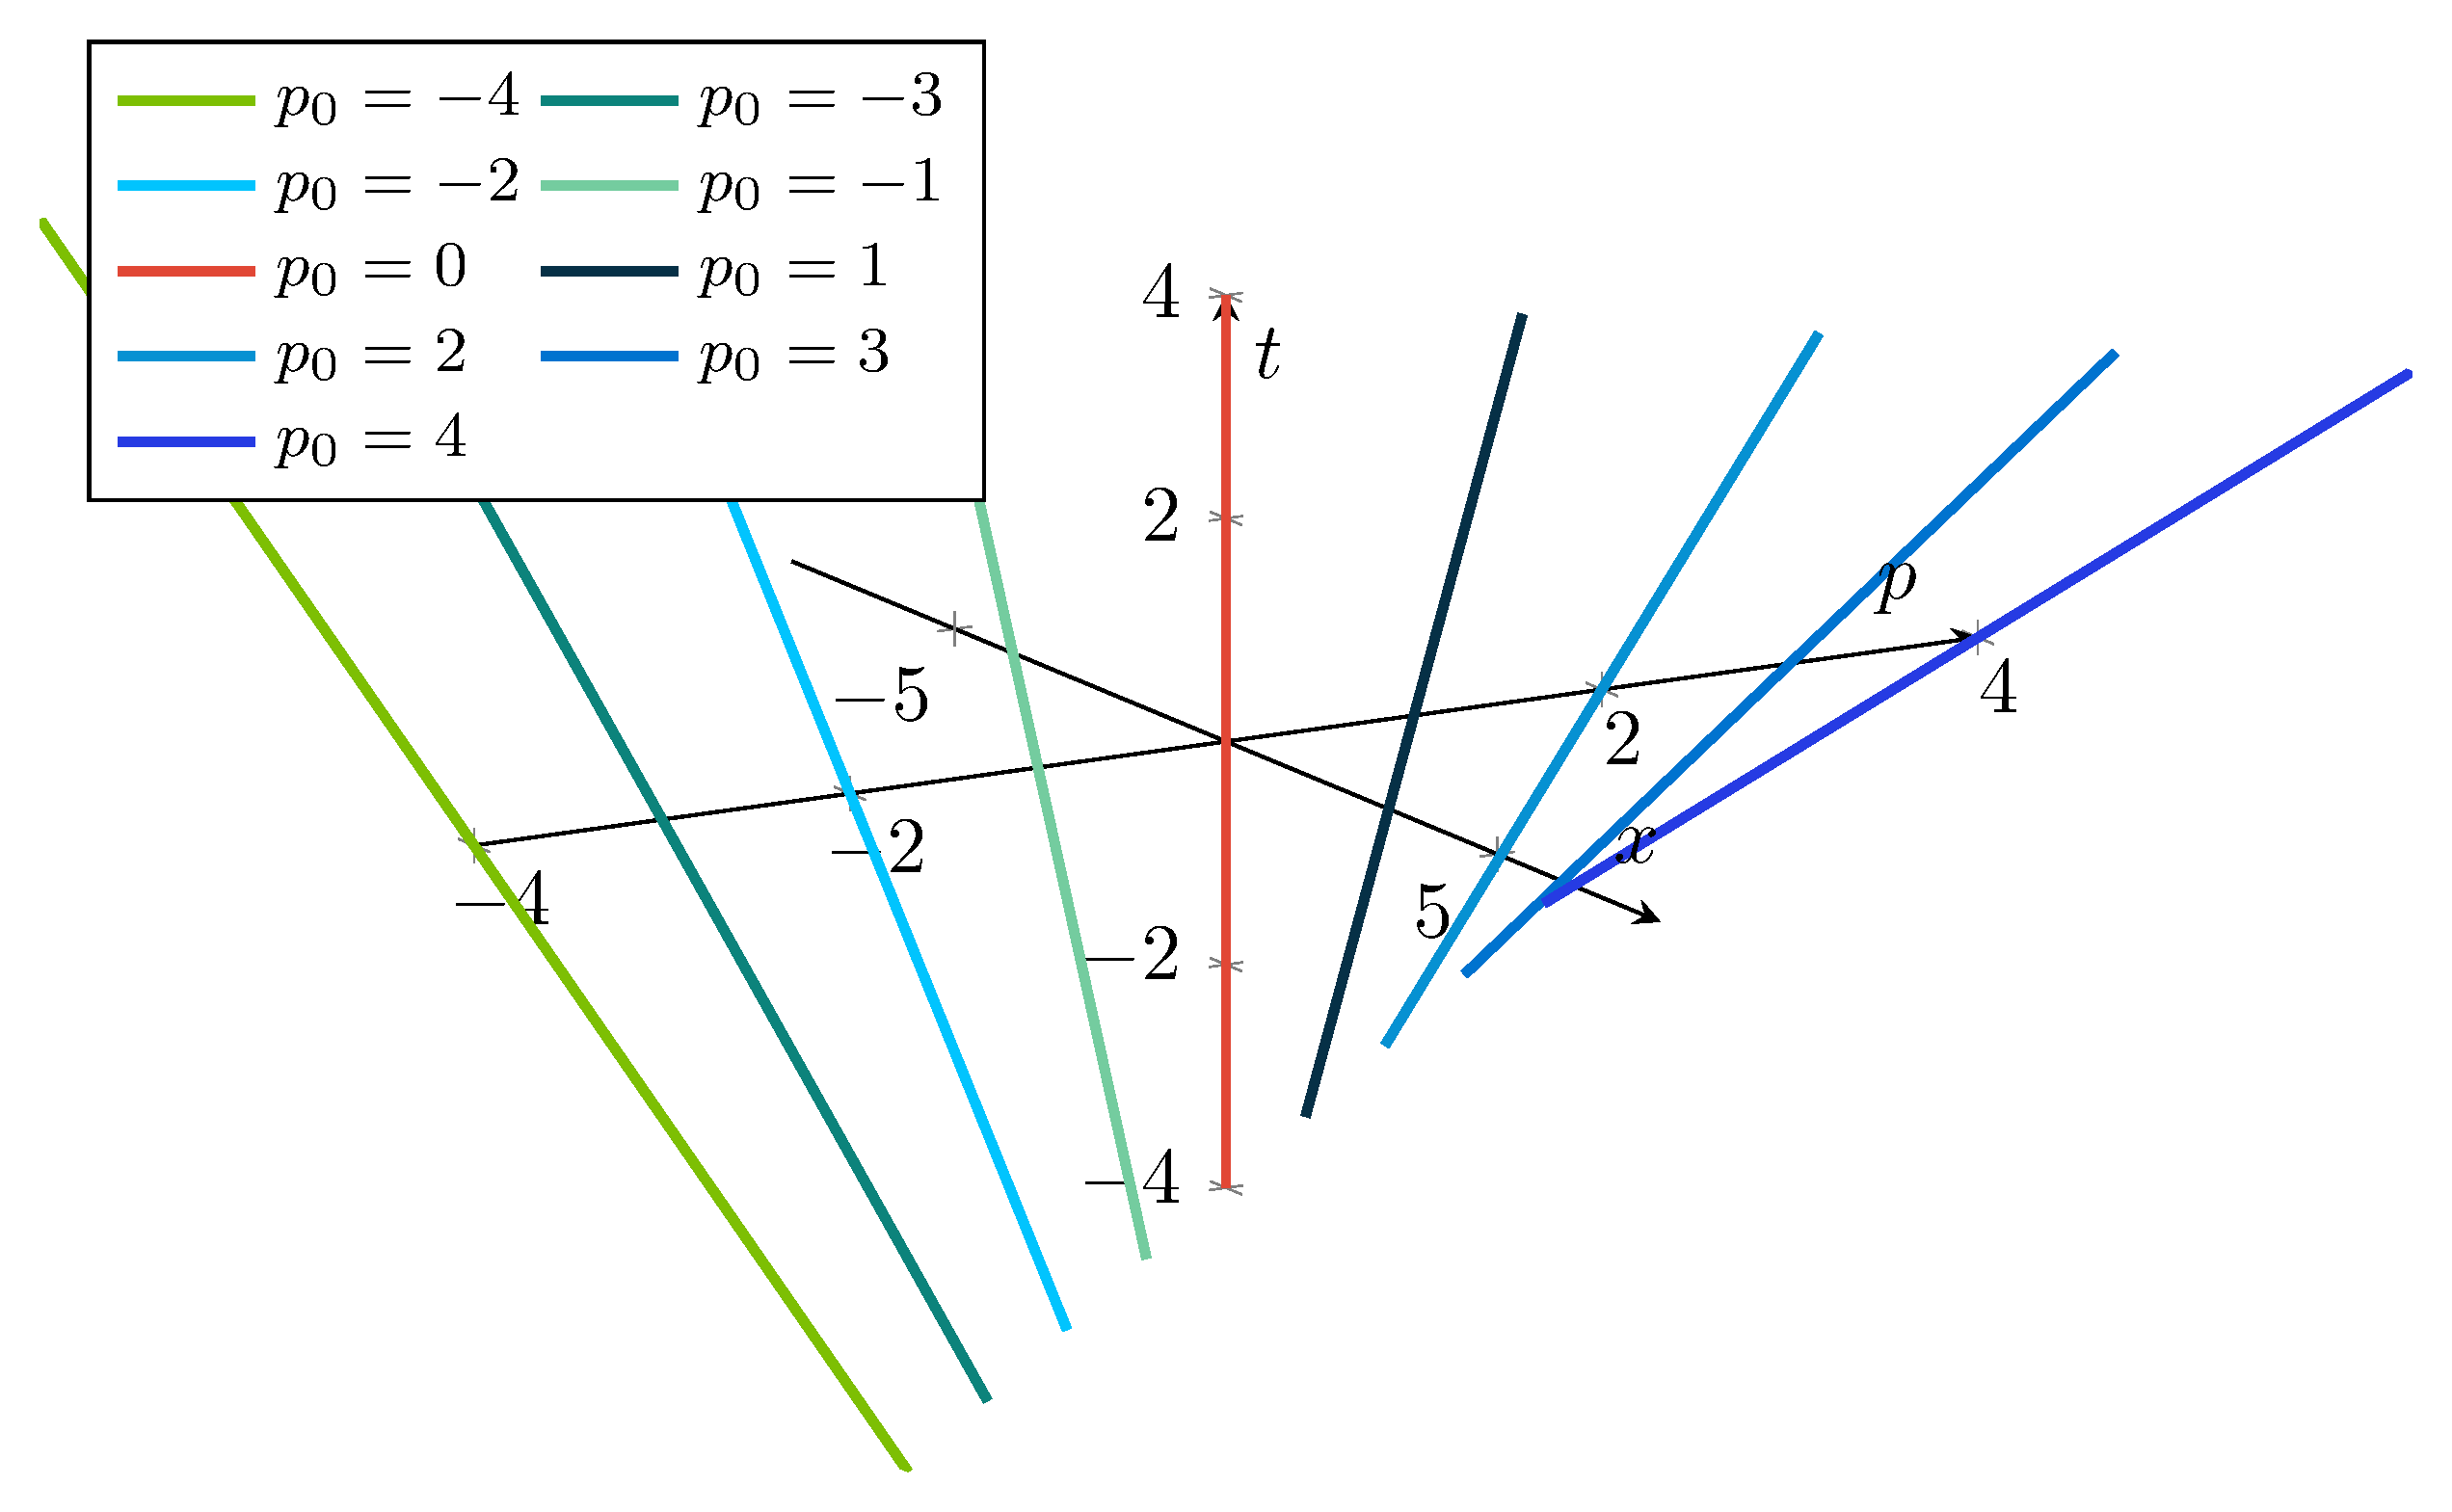
\includegraphics[width=0.9\textwidth]{grafica-1.png}
  \caption{Trayectorias rectilíneas en el espacio fase extendido \((x,p,t)\)
  para distintos valores de \(p_{0}\), con \(m=2\) y \(x_{0}=0\). Cada valor
  de \(p_{0}\) da lugar a una recta de la forma
  \( (x(t),p(t),t) = ( (p_{0}/m)t,\; p_{0},\; t ) \).}
  \label{fig:trayectorias-xtp}
\end{figure}


\begin{table}[htbp]
\centering
\caption{Parámetros de las trayectorias mostradas en la Figura~\ref{fig:trayectorias-xtp}
para \(m=2\) y \(x_{0}=0\).}
\begin{tabular}{cccc}
\toprule
$p_{0}$ &
Punto inicial $(x_{0},p_{0},0)$ &
Vector dirección $\bigl(\tfrac{p_{0}}{m},0,1\bigr)$ &
Color en la figura \\
\midrule
$-4$ & $(0,-4,0)$ & $\left(-2,0,1\right)$ &
\textcolor{Apple Green}{Apple Green} \\
$-3$ & $(0,-3,0)$ & $\left(-\tfrac{3}{2},0,1\right)$ &
\textcolor{Surfie Green}{Surfie Green} \\
$-2$ & $(0,-2,0)$ & $\left(-1,0,1\right)$ &
\textcolor{brightturquoise}{brightturquoise} \\
$-1$ & $(0,-1,0)$ & $\left(-\tfrac{1}{2},0,1\right)$ &
\textcolor{Medium Aquamarine}{Medium Aquamarine} \\
$0$  & $(0,0,0)$  & $\left(0,0,1\right)$ &
\textcolor{Cinnabar}{Cinnabar} \\
$1$  & $(0,1,0)$  & $\left(\tfrac{1}{2},0,1\right)$ &
\textcolor{Tarawera}{Tarawera} \\
$2$  & $(0,2,0)$  & $\left(1,0,1\right)$ &
\textcolor{Cerulean}{Cerulean} \\
$3$  & $(0,3,0)$  & $\left(\tfrac{3}{2},0,1\right)$ &
\textcolor{trueblue}{trueblue} \\
$4$  & $(0,4,0)$  & $\left(2,0,1\right)$ &
\textcolor{palatinateblue}{palatinateblue} \\
\bottomrule
\end{tabular}
\end{table}




%-------------------- 2) Oscilador armónico simple --------------------

\vspace{0.6cm}
\textbf{2) Oscilador armónico simple}

\begin{figure}[htbp]
\centering
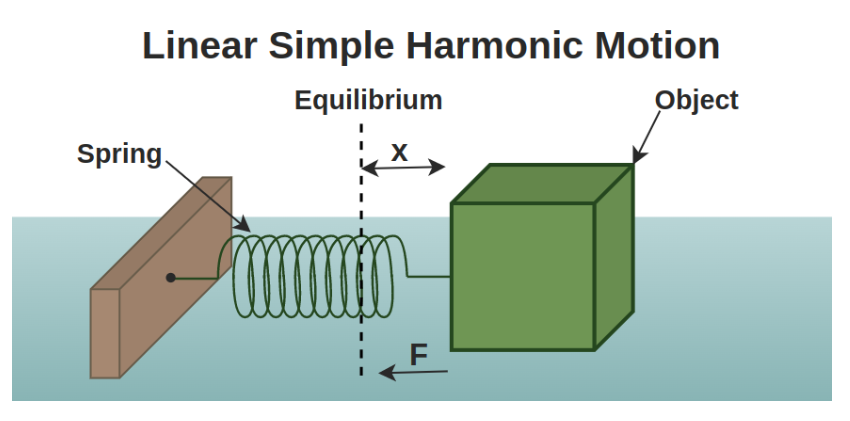
\includegraphics[width=0.75\textwidth]{oscilador_lineal.png} % <-- cambia el nombre si lo guardas distinto
\caption{
Representación esquemática del \textbf{oscilador armónico simple lineal}.  
Un objeto de masa $m$ está unido a un resorte de constante elástica $k$,
y se desplaza alrededor de la posición de equilibrio medida por la coordenada $x$.
La fuerza restauradora actúa según la ley de Hooke, $F=-kx$, dirigiéndose siempre
hacia la posición de equilibrio. Este modelo mecánico es la base del análisis
lagrangiano y hamiltoniano del movimiento oscilatorio.
}
\label{fig:oscilador-lineal}
\end{figure}


El segundo sistema que se estudia en el capítulo es el oscilador armónico simple,
cuyo Lagrangiano está dado por

\begin{equation}
\begin{split}
L(x,\dot{x},t) &= \frac{m}{2}\,\dot{x}^{2} - \frac{k}{2}\,x^{2}
\end{split}
\label{eq:L-oscilador}
\end{equation}

En la ecuación \eqref{eq:L-oscilador} se reconoce el término cinético
proporcional a $\dot{x}^{2}$ y el potencial armónico cuadrático en $x$.

De nuevo, aplicamos la transformación de Legendre que, en general, está dada por
\begin{equation}
\begin{split}
H(q,p,t) &\equiv \sum_{i=1}^{n} p_{i}\,\dot q_{i} - L(q,\dot q,t),
\qquad
p_{i} \equiv \frac{\partial L}{\partial \dot q_{i}}
\end{split}
\label{eq:legendre-general}
\end{equation}
donde al final debe expresarse $H$ únicamente en términos de $(q,p,t)$, es decir,
hay que eliminar las velocidades $\dot q_{i}$ usando las relaciones $p_{i}(\dot q)$
implícitas en \eqref{eq:legendre-general}.

En nuestro caso sólo hay una coordenada generalizada $q=x$, por lo que
la cantidad conjugada es

\begin{equation}
\begin{split}
p &= \frac{\partial L}{\partial \dot{x}}
   = \frac{\partial}{\partial \dot{x}}
     \left(\frac{m}{2}\,\dot{x}^{2} - \frac{k}{2}\,x^{2}\right)
   = m\,\dot{x}
\end{split}
\label{eq:p-oscilador}
\end{equation}

La relación \eqref{eq:p-oscilador} nos permite despejar la velocidad en función
del momento canónico:

\begin{equation}
\dot{x} = \frac{p}{m}
\label{eq:xdot-oscilador}
\end{equation}

La Hamiltoniana se define entonces como

\begin{equation}
\begin{split}
H(x,p,t)
&= p\,\dot{x} - L(x,\dot{x},t) \\[4pt]
&= p\left(\frac{p}{m}\right)
   - \left[\frac{m}{2}\left(\frac{p}{m}\right)^{2}
     - \frac{k}{2}\,x^{2}\right]
\end{split}
\label{eq:H-oscilador-intermedia}
\end{equation}

Sustituyendo \eqref{eq:xdot-oscilador} en \eqref{eq:H-oscilador-intermedia} y
simplificando, se obtiene

\begin{equation}
\begin{split}
H(x,p,t)
&= \frac{p^{2}}{m}
   - \frac{1}{2m}\,p^{2}
   + \frac{k}{2}\,x^{2} \\[4pt]
&= \frac{p^{2}}{2m} + \frac{k}{2}\,x^{2}
\end{split}
\label{eq:H-oscilador}
\end{equation}

que es la Hamiltoniana del oscilador armónico simple en términos de
las variables canónicas $(x,p)$.

Obsérvese que en \eqref{eq:H-oscilador} la energía total se escribe como la suma
de la energía cinética $T = p^{2}/2m$ y la energía potencial elástica
$V = kx^{2}/2$. Es común parametrizar la constante del resorte $k$ en términos
de la frecuencia angular $\omega$ del oscilador, mediante la relación

\[
k = m\omega^{2}
\]

Con esta notación la Hamiltoniana adopta la forma

\begin{equation}
\begin{split}
H(x,p,t) &= \frac{p^{2}}{2m} + \frac{1}{2}\,m\omega^{2}x^{2}
\end{split}
\label{eq:H-oscilador-omega}
\end{equation}

que hace explícito que el sistema es un oscilador armónico de frecuencia
angular $\omega$.

\bigskip
\textcolor{trueblue}{\textbf{Ecuaciones de Hamilton y formulación matricial}}

Las ecuaciones de Hamilton asociadas a la Hamiltoniana
\eqref{eq:H-oscilador-omega} se obtienen aplicando las definiciones

\[
\dot{x} = \frac{\partial H}{\partial p},
\qquad
\dot{p} = -\,\frac{\partial H}{\partial x}
\]

En nuestro caso resulta

\begin{equation}
\begin{split}
\dot{x} &= \frac{\partial}{\partial p}
          \left(\frac{p^{2}}{2m} + \frac{1}{2}\,m\omega^{2}x^{2}\right)
        = \frac{p}{m} \\[4pt]
\dot{p} &= -\,\frac{\partial}{\partial x}
          \left(\frac{p^{2}}{2m} + \frac{1}{2}\,m\omega^{2}x^{2}\right)
        = -\,m\omega^{2}x
\end{split}
\label{eq:ecuaciones-Hamilton-oscilador}
\end{equation}

Se trata de un sistema lineal de ecuaciones diferenciales de primer orden con
coeficientes constantes. Es conveniente introducir el vector de fase

\[
\mathbf{X}(t) \equiv
\begin{pmatrix}
x(t) \\[4pt]
p(t)
\end{pmatrix}
\]

para escribir el sistema \eqref{eq:ecuaciones-Hamilton-oscilador} de forma
compacta. A partir de esas ecuaciones se observa que

\[
\frac{d}{dt}
\begin{pmatrix}
x \\[4pt]
p
\end{pmatrix}
=
\begin{pmatrix}
\dot{x} \\[4pt]
\dot{p}
\end{pmatrix}
=
\begin{pmatrix}
0 & \dfrac{1}{m} \\[6pt]
-\,m\omega^{2} & 0
\end{pmatrix}
\begin{pmatrix}
x \\[4pt]
p
\end{pmatrix}
\]

Esto nos lleva a la ecuación matricial

\begin{equation}
\frac{d}{dt}
\begin{pmatrix}
x \\[4pt]
p
\end{pmatrix}
=
\begin{pmatrix}
0 & \dfrac{1}{m} \\[6pt]
-\,m\omega^{2} & 0
\end{pmatrix}
\begin{pmatrix}
x \\[4pt]
p
\end{pmatrix}
\equiv
A
\begin{pmatrix}
x \\[4pt]
p
\end{pmatrix}
\label{eq:sistema-matricial-oscilador}
\end{equation}

donde hemos introducido la matriz

\begin{equation}
A =
\begin{pmatrix}
0 & \dfrac{1}{m} \\[6pt]
-\,m\omega^{2} & 0
\end{pmatrix}
\label{eq:matriz-A-oscilador}
\end{equation}

La ecuación \eqref{eq:sistema-matricial-oscilador} es una ecuación diferencial
lineal de primer orden para el vector $\mathbf{X}(t)$ con matriz de coeficientes
constante $A$. Existe un resultado estándar para este tipo de sistemas: si
$\mathbf{X}(t)$ satisface

\[
\dot{\mathbf{X}}(t) = A\,\mathbf{X}(t),
\qquad
\mathbf{X}(0) = \mathbf{X}_{0},
\]

entonces la solución se puede escribir mediante la exponencial matricial como

\[
\mathbf{X}(t) = e^{At}\,\mathbf{X}_{0}
\]

En nuestro caso, $\mathbf{X}_{0} = (x_{0},p_{0})^{T}$ representa la posición y
el momento al tiempo inicial $t=0$. Por lo tanto, la solución formal del sistema
\eqref{eq:sistema-matricial-oscilador} es

\begin{equation}
\begin{pmatrix}
x(t) \\[4pt]
p(t)
\end{pmatrix}
=
e^{At}
\begin{pmatrix}
x_{0} \\[4pt]
p_{0}
\end{pmatrix}
\label{eq:solucion-matricial-formal}
\end{equation}

La exponencial matricial $e^{At}$ se introduce a partir de la misma construcción
analítica que en el caso escalar. Recordemos que toda función suficientemente
suave puede desarrollarse en una serie de \textbf{Taylor} alrededor de un punto
$a$ mediante

\[
f(x) = \sum_{n=0}^{\infty} \frac{f^{(n)}(a)}{n!}\,(x-a)^{n}.
\]

Cuando el punto de expansión es $a=0$, esta expresión recibe el nombre de
\textbf{serie de Maclaurin}. En particular, para la función exponencial se tiene

\[
e^{x} = \sum_{n=0}^{\infty} \frac{x^{n}}{n!},
\]

pues todas las derivadas de $e^{x}$ coinciden con la propia función y
$f^{(n)}(0)=1$ para todo $n$.

La clave del método matricial consiste en extender esta definición al caso en que
el argumento ya no es un número, sino una matriz. Dado que la serie de Maclaurin
de $e^{x}$ es absolutamente convergente para todo $x\in\mathbb{R}$ (e incluso para
todo número complejo), es posible sustituir $\textcolor{Lochmara}{\boldsymbol{x}}$ por la matriz $\textcolor{orange(colorwheel)}{\boldsymbol{A}}t$ sin perder
convergencia: cada entrada de la serie resultante es una serie numérica bien
definida. De esta manera se define la \textbf{exponencial matricial} como

\begin{equation}
e^{At} \equiv \sum_{n=0}^{\infty} \frac{A^{n} t^{n}}{n!},
\label{eq:def-exp-At}
\end{equation}

lo cual constituye la generalización natural de la exponencial escalar. Esta
definición garantiza, además, que $e^{At}$ es la solución fundamental del sistema
lineal homogéneo $\dot{\mathbf{X}} = A\mathbf{X}$, satisfaciendo

\[
\frac{d}{dt}e^{At} = A\,e^{At},
\qquad
e^{A\cdot 0} = I.
\]

Nuestro objetivo es ahora calcular explícitamente esta exponencial para la matriz
$A$ asociada al oscilador armónico simple.


\bigskip
\textcolor{trueblue}{\textbf{Cálculo de las potencias de $A$}}

Para hacer explícita la solución necesitamos analizar la forma de las potencias
de $A$, ya que todas aparecen en la serie \eqref{eq:def-exp-At}. Comencemos
calculando $A^{2}$. Usando \eqref{eq:matriz-A-oscilador} se tiene

\begin{equation}
\begin{split}
A^{2}
&=
\begin{pmatrix}
0 & \dfrac{1}{m} \\[6pt]
-\,m\omega^{2} & 0
\end{pmatrix}
\begin{pmatrix}
0 & \dfrac{1}{m} \\[6pt]
-\,m\omega^{2} & 0
\end{pmatrix} \\[8pt]
&=
\begin{pmatrix}
0\cdot 0 + \dfrac{1}{m}\left(-\,m\omega^{2}\right) &
0\cdot \dfrac{1}{m} + \dfrac{1}{m}\cdot 0 \\[6pt]
-\,m\omega^{2}\cdot 0 + 0\left(-\,m\omega^{2}\right) &
-\,m\omega^{2}\cdot \dfrac{1}{m} + 0\cdot 0
\end{pmatrix} \\[8pt]
&=
\begin{pmatrix}
-\,\omega^{2} & 0 \\[4pt]
0 & -\,\omega^{2}
\end{pmatrix}
= -\,\omega^{2}\,I
\end{split}
\label{eq:A-cuadrada-oscilador}
\end{equation}

donde $I$ denota la matriz identidad de dimensión $2\times 2$. El resultado
\eqref{eq:A-cuadrada-oscilador} es especialmente simple: al multiplicar $A$ por
sí misma se obtiene una matriz proporcional a la identidad. Esta propiedad es
la que hace que la exponencial matricial de $A$ se exprese en términos de
funciones trigonométricas.

A partir de \eqref{eq:A-cuadrada-oscilador} podemos obtener fácilmente las
potencias superiores. Por ejemplo,

\[
A^{3} = A^{2}A = \left(-\,\omega^{2}I\right)A = -\,\omega^{2}A
\]

y

\[
A^{4} = A^{2}A^{2} = \left(-\,\omega^{2}I\right)\left(-\,\omega^{2}I\right)
= \omega^{4}I
\]

Si continuamos este procedimiento, se observa que las potencias pares de $A$
son siempre proporcionales a la identidad y las potencias impares son siempre
proporcionales a $A$. En general se cumple que

\begin{equation}
A^{2n} = (-1)^{n}\,\omega^{2n} I,
\qquad
A^{2n+1} = (-1)^{n}\,\omega^{2n} A,
\qquad n=0,1,2,\dots
\label{eq:potencias-A-generales}
\end{equation}

Esta relación resume el patrón completo de las potencias de la matriz $A$.

\bigskip
\textcolor{trueblue}{\textbf{Separación en términos pares e impares en $e^{At}$}}

Sustituyendo \eqref{eq:potencias-A-generales} en la definición de la exponencial
matricial \eqref{eq:def-exp-At} y separando explícitamente los términos pares e
impares en la suma, obtenemos

\begin{equation}
\begin{split}
e^{At}
&= \sum_{n=0}^{\infty} \frac{A^{n} t^{n}}{n!} \\[4pt]
&= \sum_{n=0}^{\infty} \frac{A^{2n} t^{2n}}{(2n)!}
   \;+\; \sum_{n=0}^{\infty} \frac{A^{2n+1} t^{2n+1}}{(2n+1)!} \\[4pt]
&= \sum_{n=0}^{\infty}
   \frac{(-1)^{n}\omega^{2n} t^{2n}}{(2n)!}\,I
   \;+\;
   \sum_{n=0}^{\infty}
   \frac{(-1)^{n}\omega^{2n} t^{2n+1}}{(2n+1)!}\,A
\end{split}
\label{eq:exp-At-series}
\end{equation}

Para ver con toda claridad la estructura de estas series, expandimos los primeros
términos de cada una. En la parte que multiplica a $I$, tomando $n=0,1,2,\dots$:

\[
\sum_{n=0}^{\infty}
\frac{(-1)^{n}\omega^{2n} t^{2n}}{(2n)!}
=
1
- \frac{(\omega t)^{2}}{2!}
+ \frac{(\omega t)^{4}}{4!}
- \cdots
\]

De modo que el término “par” de $e^{At}$ se escribe como

\[
I\sum_{n=0}^{\infty}
\frac{(-1)^{n}\omega^{2n} t^{2n}}{(2n)!}
=
I\left[1 - \frac{(\omega t)^{2}}{2!}
          + \frac{(\omega t)^{4}}{4!}
          - \cdots \right]
\]

Por otro lado, en la parte que multiplica a $A$ obtenemos

\[
\sum_{n=0}^{\infty}
\frac{(-1)^{n}\omega^{2n} t^{2n+1}}{(2n+1)!}
=
t
- \frac{\omega^{2} t^{3}}{3!}
+ \frac{\omega^{4} t^{5}}{5!}
- \cdots
\]

y por lo tanto el término “impar” de $e^{At}$ es

\[
A\sum_{n=0}^{\infty}
\frac{(-1)^{n}\omega^{2n} t^{2n+1}}{(2n+1)!}
=
A\left[
t
- \frac{\omega^{2} t^{3}}{3!}
+ \frac{\omega^{4} t^{5}}{5!}
- \cdots
\right]
\]

Reuniendo ambas contribuciones, la expansión explícita de la exponencial matricial
queda

\begin{equation}
\begin{split}
e^{At}
&=
I\left[
1 - \frac{(\omega t)^{2}}{2!}
  + \frac{(\omega t)^{4}}{4!}
  - \cdots
\right]
+
A\left[
t
- \frac{\omega^{2} t^{3}}{3!}
+ \frac{\omega^{4} t^{5}}{5!}
- \cdots
\right]
\end{split}
\label{eq:exp-At-expandida-1}
\end{equation}

Para hacer aparecer las funciones trigonométricas, reescribimos la segunda serie
en términos de potencias de $(\omega t)$. Nótese que

\[
\omega^{2n} t^{2n+1}
= \frac{(\omega t)^{2n+1}}{\omega} \quad \text{es decir, multiplicamos por un}\, 1 = \frac{\omega}{\omega}
\]

de modo que

\[
\sum_{n=0}^{\infty}
\frac{(-1)^{n}\omega^{2n} t^{2n+1}}{(2n+1)!}
=
\frac{1}{\omega}
\sum_{n=0}^{\infty}
\frac{(-1)^{n}(\omega t)^{2n+1}}{(2n+1)!}
\]

y por lo tanto

\[
A\left[
t
- \frac{\omega^{2} t^{3}}{3!}
+ \frac{\omega^{4} t^{5}}{5!}
- \cdots
\right]
=
\frac{A}{\omega}
\left[
\omega t
- \frac{(\omega t)^{3}}{3!}
+ \frac{(\omega t)^{5}}{5!}
- \cdots
\right]
\]

Con esta reescritura, la expresión \eqref{eq:exp-At-expandida-1} se puede
presentar de forma compacta como

\begin{equation}
\begin{split}
e^{At}
&=
I\left[
1 - \frac{(\omega t)^{2}}{2!}
  + \frac{(\omega t)^{4}}{4!}
  - \cdots
\right]
+
\frac{A}{\omega}
\left[
\omega t
- \frac{(\omega t)^{3}}{3!}
+ \frac{(\omega t)^{5}}{5!}
- \cdots
\right]
\end{split}
\label{eq:exp-At-expandida-2}
\end{equation}

En \eqref{eq:exp-At-expandida-2} se ve claramente que:

\begin{itemize}
  \item[$\bullet$] la serie que multiplica a $I$ contiene únicamente potencias
  \emph{pares} de $(\omega t)$
  \item[$\bullet$] la serie que multiplica a $A/\omega$ contiene únicamente potencias
  \emph{impares} de $(\omega t)$
\end{itemize}

Este comportamiento es precisamente el que caracteriza a las series de
\textbf{Taylor} de las funciones trigonométricas alrededor de $t=0$:

\begin{equation}
\cos(\omega t) =
\sum_{n=0}^{\infty} \frac{(-1)^{n}}{(2n)!}(\omega t)^{2n},
\qquad
\sin(\omega t) =
\sum_{n=0}^{\infty} \frac{(-1)^{n}}{(2n+1)!}(\omega t)^{2n+1}
\end{equation}

La primera serie involucra únicamente términos pares, mientras que la segunda
involucra únicamente términos impares. En consecuencia,

\[
\sum_{n=0}^{\infty}
\frac{(-1)^{n}(\omega t)^{2n}}{(2n)!}
= \cos(\omega t),
\qquad
\sum_{n=0}^{\infty}
\frac{(-1)^{n}(\omega t)^{2n+1}}{(2n+1)!}
= \sin(\omega t)
\]

y la expresión \eqref{eq:exp-At-expandida-2} se reduce finalmente a

\begin{equation}
\begin{split}
e^{At}
&= I\cos(\omega t) + \frac{A}{\omega}\,\sin(\omega t)
\end{split}
\label{eq:exp-At-final}
\end{equation}

Esta identidad muestra de manera transparente cómo la exponencial matricial
$e^{At}$ combina las series pares e impares en términos de $\cos(\omega t)$
y $\sin(\omega t)$, reflejando la naturaleza oscilatoria del oscilador
armónico simple.


\bigskip
\textcolor{trueblue}{\textbf{Obtención  de $x(t)$ y $p(t)$}}

Sustituyendo \eqref{eq:exp-At-final} en la solución formal
\eqref{eq:solucion-matricial-formal} encontramos

\begin{equation}
\begin{split}
\begin{pmatrix}
x(t) \\[4pt]
p(t)
\end{pmatrix}
&=
\left[
I\cos(\omega t) + \frac{A}{\omega}\,\sin(\omega t)
\right]
\begin{pmatrix}
x_{0} \\[4pt]
p_{0}
\end{pmatrix}
\end{split}
\label{eq:xp-con-exp-At}
\end{equation}

Para evaluar el lado derecho de \eqref{eq:xp-con-exp-At} calculamos por separado
la acción de $I$ y de $A$ sobre el vector inicial. Para la identidad se tiene

\[
I
\begin{pmatrix}
x_{0} \\[4pt]
p_{0}
\end{pmatrix}
=
\begin{pmatrix}
x_{0} \\[4pt]
p_{0}
\end{pmatrix}
\]

Mientras que para $A$ usamos nuevamente \eqref{eq:matriz-A-oscilador}:

\[
A
\begin{pmatrix}
x_{0} \\[4pt]
p_{0}
\end{pmatrix}
=
\begin{pmatrix}
0 & \dfrac{1}{m} \\[6pt]
-\,m\omega^{2} & 0
\end{pmatrix}
\begin{pmatrix}
x_{0} \\[4pt]
p_{0}
\end{pmatrix}
=
\begin{pmatrix}
\dfrac{p_{0}}{m} \\[6pt]
-\,m\omega^{2}x_{0}
\end{pmatrix}
\]

Con estos resultados, la ecuación \eqref{eq:xp-con-exp-At} se traduce en

\begin{equation}
\begin{split}
\begin{pmatrix}
x(t) \\[4pt]
p(t)
\end{pmatrix}
&=
\cos(\omega t)
\begin{pmatrix}
x_{0} \\[4pt]
p_{0}
\end{pmatrix}
+
\frac{\sin(\omega t)}{\omega}
\begin{pmatrix}
\dfrac{p_{0}}{m} \\[6pt]
-\,m\omega^{2}x_{0}
\end{pmatrix}
\end{split}
\end{equation}

es decir,

\begin{equation}
\begin{split}
x(t)
&= x_{0}\cos(\omega t)
   + \frac{1}{\omega}\left(\frac{p_{0}}{m}\right)\sin(\omega t) \\[4pt]
p(t)
&= p_{0}\cos(\omega t)
   + \frac{1}{\omega}\left(-\,m\omega^{2}x_{0}\right)\sin(\omega t)
\end{split}
\label{eq:xp-soluciones-matriciales}
\end{equation}

Simplificando los factores se obtiene

\begin{equation}
\begin{split}
x(t)
&= x_{0}\cos(\omega t)
   + \frac{p_{0}}{m\omega}\,\sin(\omega t) \\[4pt]
p(t)
&= p_{0}\cos(\omega t)
   - m\omega x_{0}\,\sin(\omega t)
\end{split}
\end{equation}

Si introducimos la velocidad inicial $v_{0} = \dot{x}(0) = p_{0}/m$, la primera
de estas ecuaciones adopta la forma más habitual

\begin{equation}
\begin{split}
x(t)
&= x_{0}\cos(\omega t)
   + \frac{v_{0}}{\omega}\,\sin(\omega t)
\end{split}
\label{eq:x-solucion-matriz}
\end{equation}

Por otro lado, la expresión para $p(t)$ confirma que en todo instante se cumple

\[
p(t) = m\,\dot{x}(t)
\]

lo cual es consistente con la definición del momento canónico y verifica que la
formulación matricial reproduce correctamente la dinámica del oscilador armónico
simple.

\vspace{0.4cm}
\textcolor{trueblue}{\textbf{Trayectorias en el espacio fase $(x,p)$}}

A partir de las soluciones explícitas obtenidas en \eqref{eq:xp-soluciones-matriciales},
las trayectorias del oscilador armónico simple en el espacio fase se describen
mediante la curva paramétrica

\[
x(t) = x_{0}\cos(\omega t) + \frac{p_{0}}{m\omega}\sin(\omega t),
\qquad
p(t) = p_{0}\cos(\omega t) - m\omega x_{0}\sin(\omega t)
\]

donde el parámetro es el tiempo $t$.  
Una característica notable del movimiento oscilatorio es que, a diferencia de la
partícula libre, las trayectorias en el plano $(x,p)$ no son rectas sino
\emph{curvas cerradas}. Para hacer esto explícito eliminemos el parámetro $t$.

Multiplicamos la primera ecuación por $m\omega$ y escribimos

\[
m\omega\,x(t)
= m\omega x_{0}\cos(\omega t)
  + p_{0}\sin(\omega t)
\]

Mientras que la ecuación para $p(t)$ se reescribe como

\[
p(t)
= p_{0}\cos(\omega t)
  - m\omega x_{0}\sin(\omega t)
\]

Denotemos

\[
X(t) \equiv m\omega\,x(t),
\qquad
P(t) \equiv p(t)
\]

Entonces el sistema adopta la forma matricial

\[
\begin{pmatrix}
X(t) \\[4pt]
P(t)
\end{pmatrix}
=
\begin{pmatrix}
m\omega x_{0} \\[4pt]
p_{0}
\end{pmatrix}
\cos(\omega t)
+
\begin{pmatrix}
p_{0} \\[4pt]
-\,m\omega x_{0}
\end{pmatrix}
\sin(\omega t)
\]

Lo anterior muestra que el vector $(X(t),P(t))$ describe una rotación uniforme
en el plano, con velocidad angular $\omega$.  
Para ver la curva geométrica, usamos la identidad trigonométrica básica
$\cos^{2}(\omega t)+\sin^{2}(\omega t)=1$ y combinamos ambos componentes. Se obtiene

\[
\frac{X(t)^{2}}{(m\omega x_{0})^{2} + p_{0}^{2}}
+
\frac{P(t)^{2}}{(m\omega x_{0})^{2} + p_{0}^{2}}
= 1
\]

Sustituyendo $X(t) = m\omega x(t)$ y simplificando,

\begin{equation}
\frac{x(t)^{2}}{x_{0}^{2} + \left(\tfrac{p_{0}}{m\omega}\right)^{2}}
+
\frac{p(t)^{2}}{p_{0}^{2} + (m\omega x_{0})^{2}}
= 1
\label{eq:elipse-oscilador}
\end{equation}

Esta es la ecuación de una \textbf{elipse} en el plano $(x,p)$. Cada elipse
corresponde a un valor fijo de la energía total
\[
H = \frac{p_{0}^{2}}{2m} + \frac{1}{2}m\omega^{2}x_{0}^{2},
\]
de modo que las curvas de nivel de la Hamiltoniana coinciden con las trayectorias
en el espacio fase.

En la Figura~\ref{fig:oscilador-xp} se muestran varias de estas órbitas
cerradas para distintos pares de condiciones iniciales $(x_{0},p_{0})$.

\begin{figure}[H]
\centering
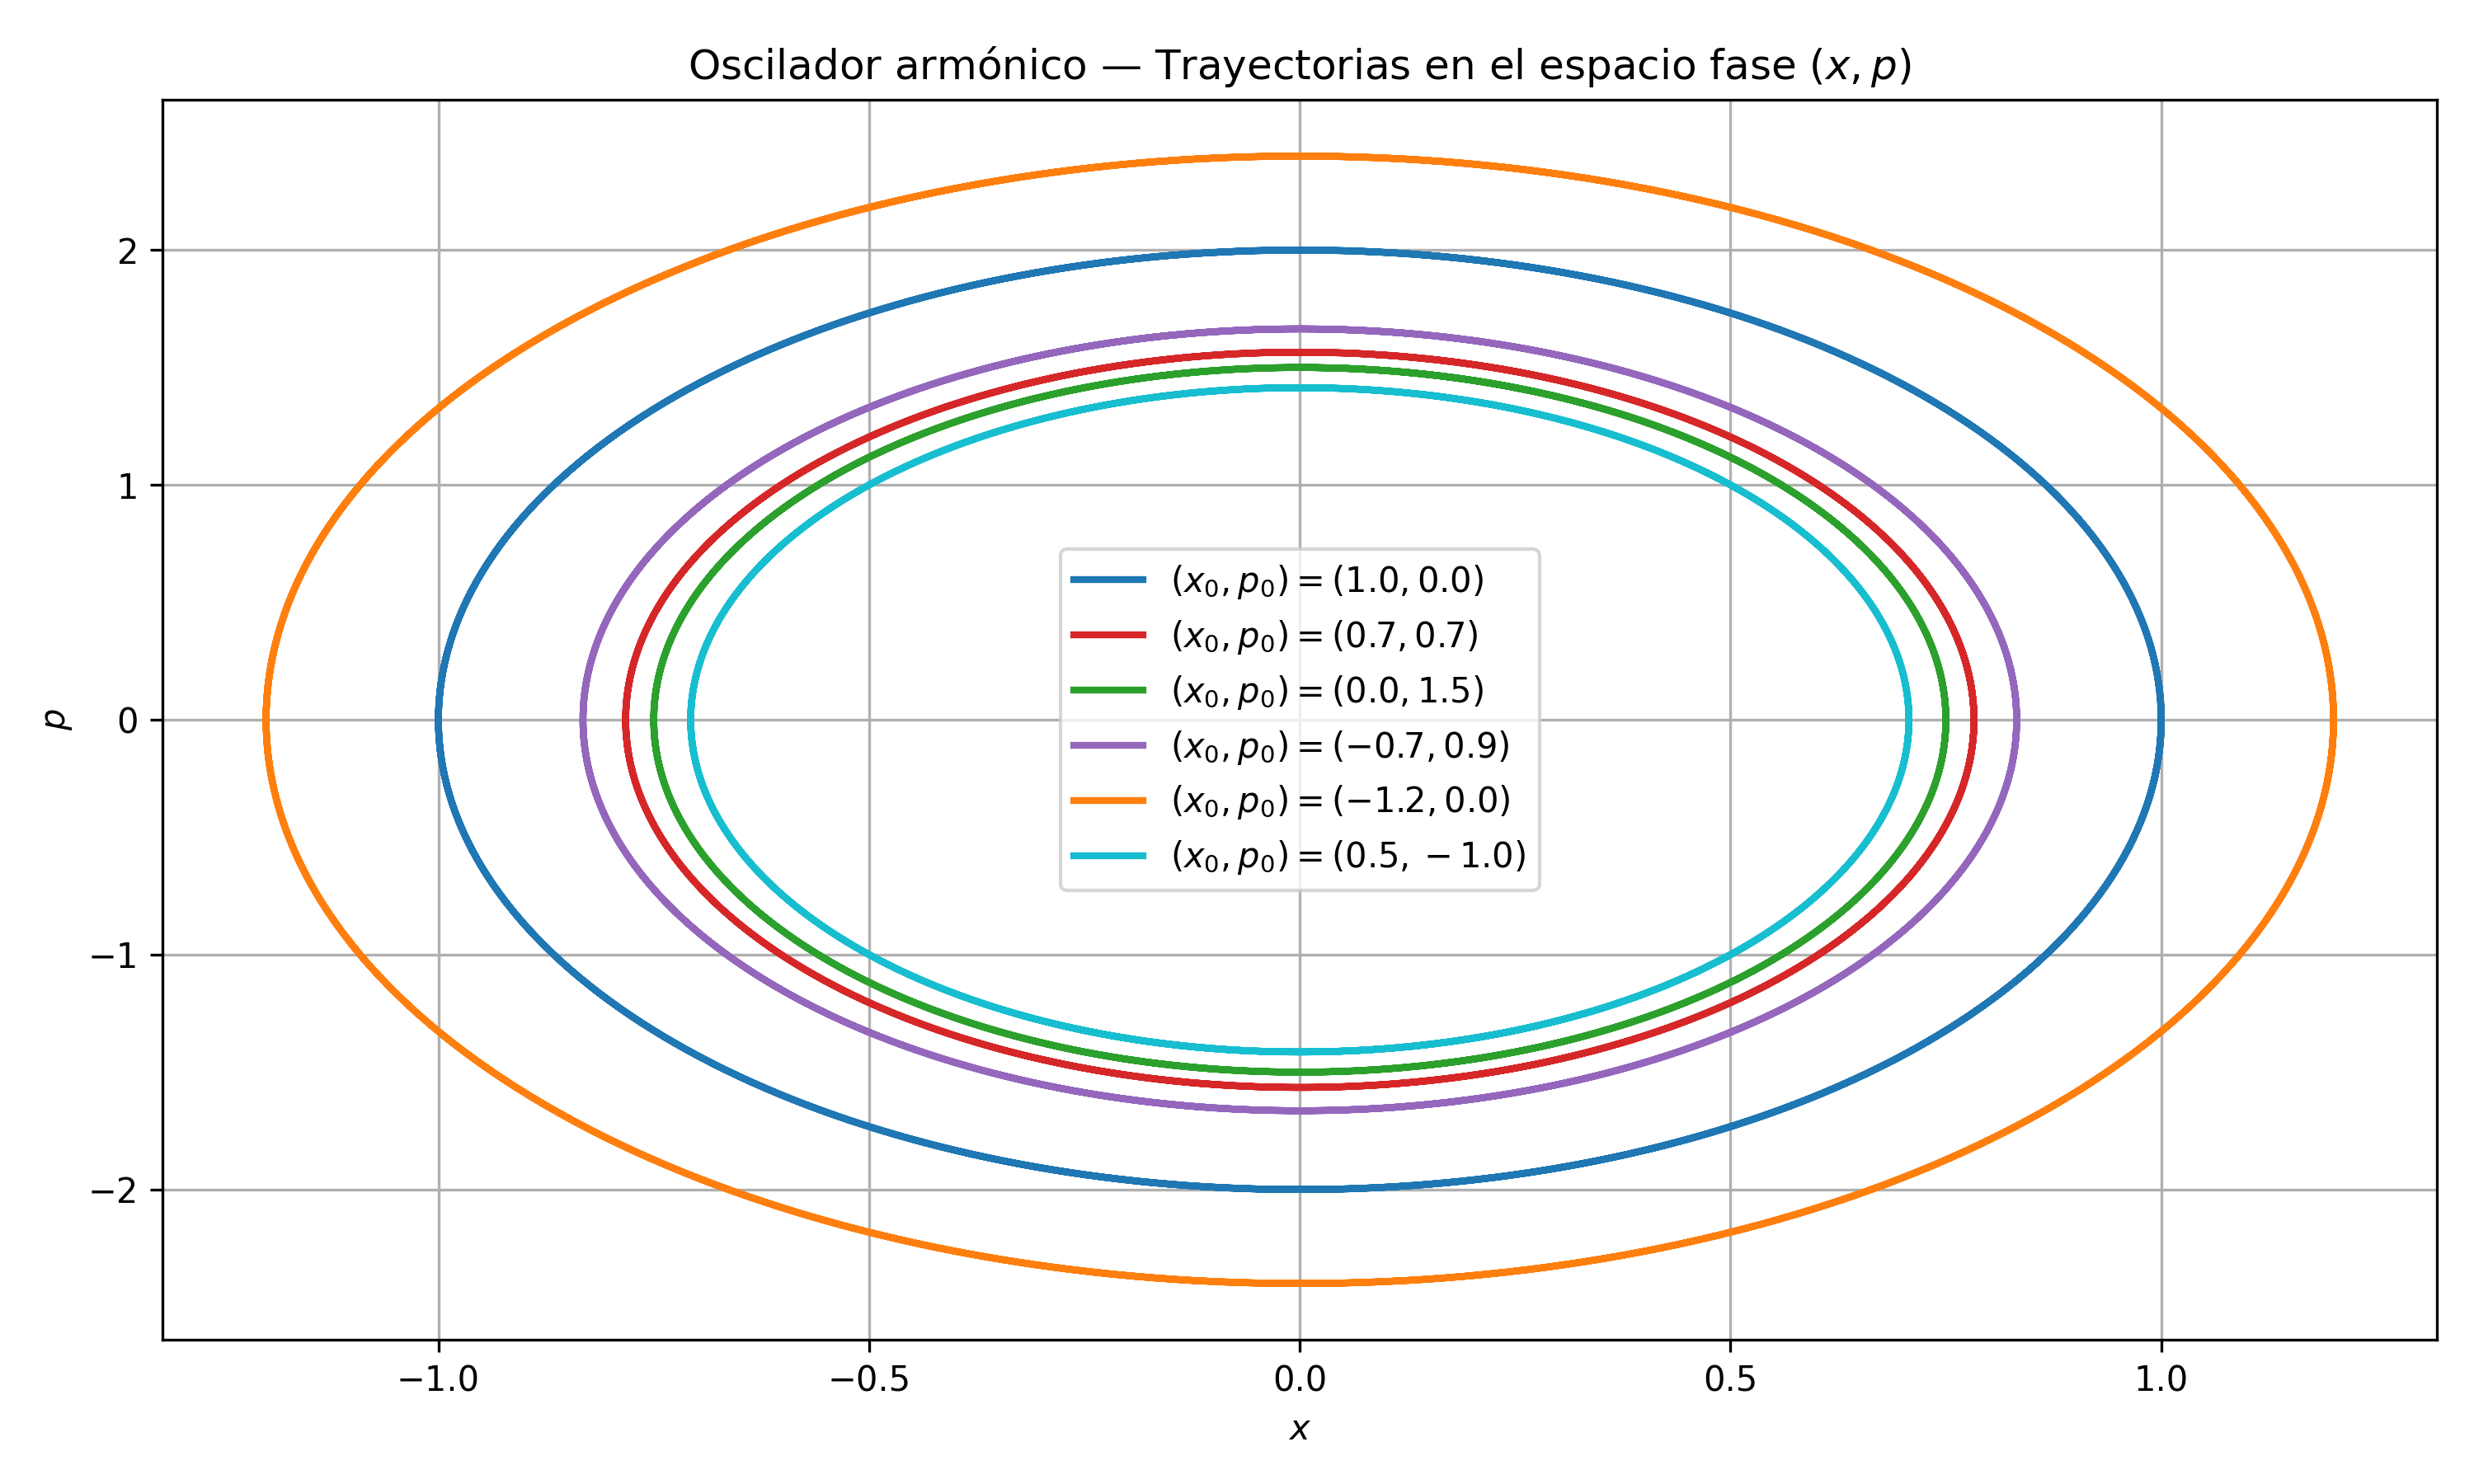
\includegraphics[width=0.9\textwidth]{oscilador_xp.png}
\caption{
Trayectorias del \textbf{oscilador armónico simple} en el espacio fase
\((x,p)\) para distintos valores iniciales \((x_{0},p_{0})\).  
Cada curva cerrada es una elipse dada por \eqref{eq:elipse-oscilador} y
representa una órbita de energía constante
\(H = p^{2}/2m + m\omega^{2}x^{2}/2\).  
La figura fue generada mediante un script en \texttt{Python} usando la
biblioteca \texttt{matplotlib}, tomando \(m=1\), \(\omega=1\) y las
condiciones iniciales indicadas en la leyenda.}
\label{fig:oscilador-xp}
\end{figure}

\bigskip
\textcolor{trueblue}{\textbf{Trayectorias en el espacio fase extendido $(x,p,t)$}}

Si ahora incorporamos el tiempo como tercera coordenada, las trayectorias toman
la forma paramétrica tridimensional

\[
(x(t),\,p(t),\,t),
\]

donde $(x(t),p(t))$ sigue describiendo la elipse \eqref{eq:elipse-oscilador},
mientras que $t$ crece de manera uniforme.  
La inclusión del tiempo genera una curva \emph{helicoidal} en el espacio
$(x,p,t)$: al proyectarla sobre el plano $(x,p)$ se recupera la elipse, mientras
que la coordenada vertical $t$ hace que la trayectoria ascienda monótonamente.  

Geométricamente:

\begin{itemize}
  \item[$\bullet$] las oscilaciones en $x$ y $p$ son periódicas con periodo $T=2\pi/\omega$;
  \item[$\bullet$] el tiempo $t$ actúa como “altura”, por lo que la curva nunca
    se cierra en $(x,p,t)$;
  \item[$\bullet$] las proyecciones sobre los planos $(x,t)$ y $(p,t)$ muestran
    oscilaciones sinusoidales;
  \item[$\bullet$] la energía $H$ permanece constante a lo largo de toda la evolución.
\end{itemize}

En la Figura~\ref{fig:oscilador-xpt} se ilustran estas trayectorias helicoidales
para los mismos conjuntos de condiciones iniciales utilizados en la
Figura~\ref{fig:oscilador-xp}.

\begin{figure}[H]
\centering
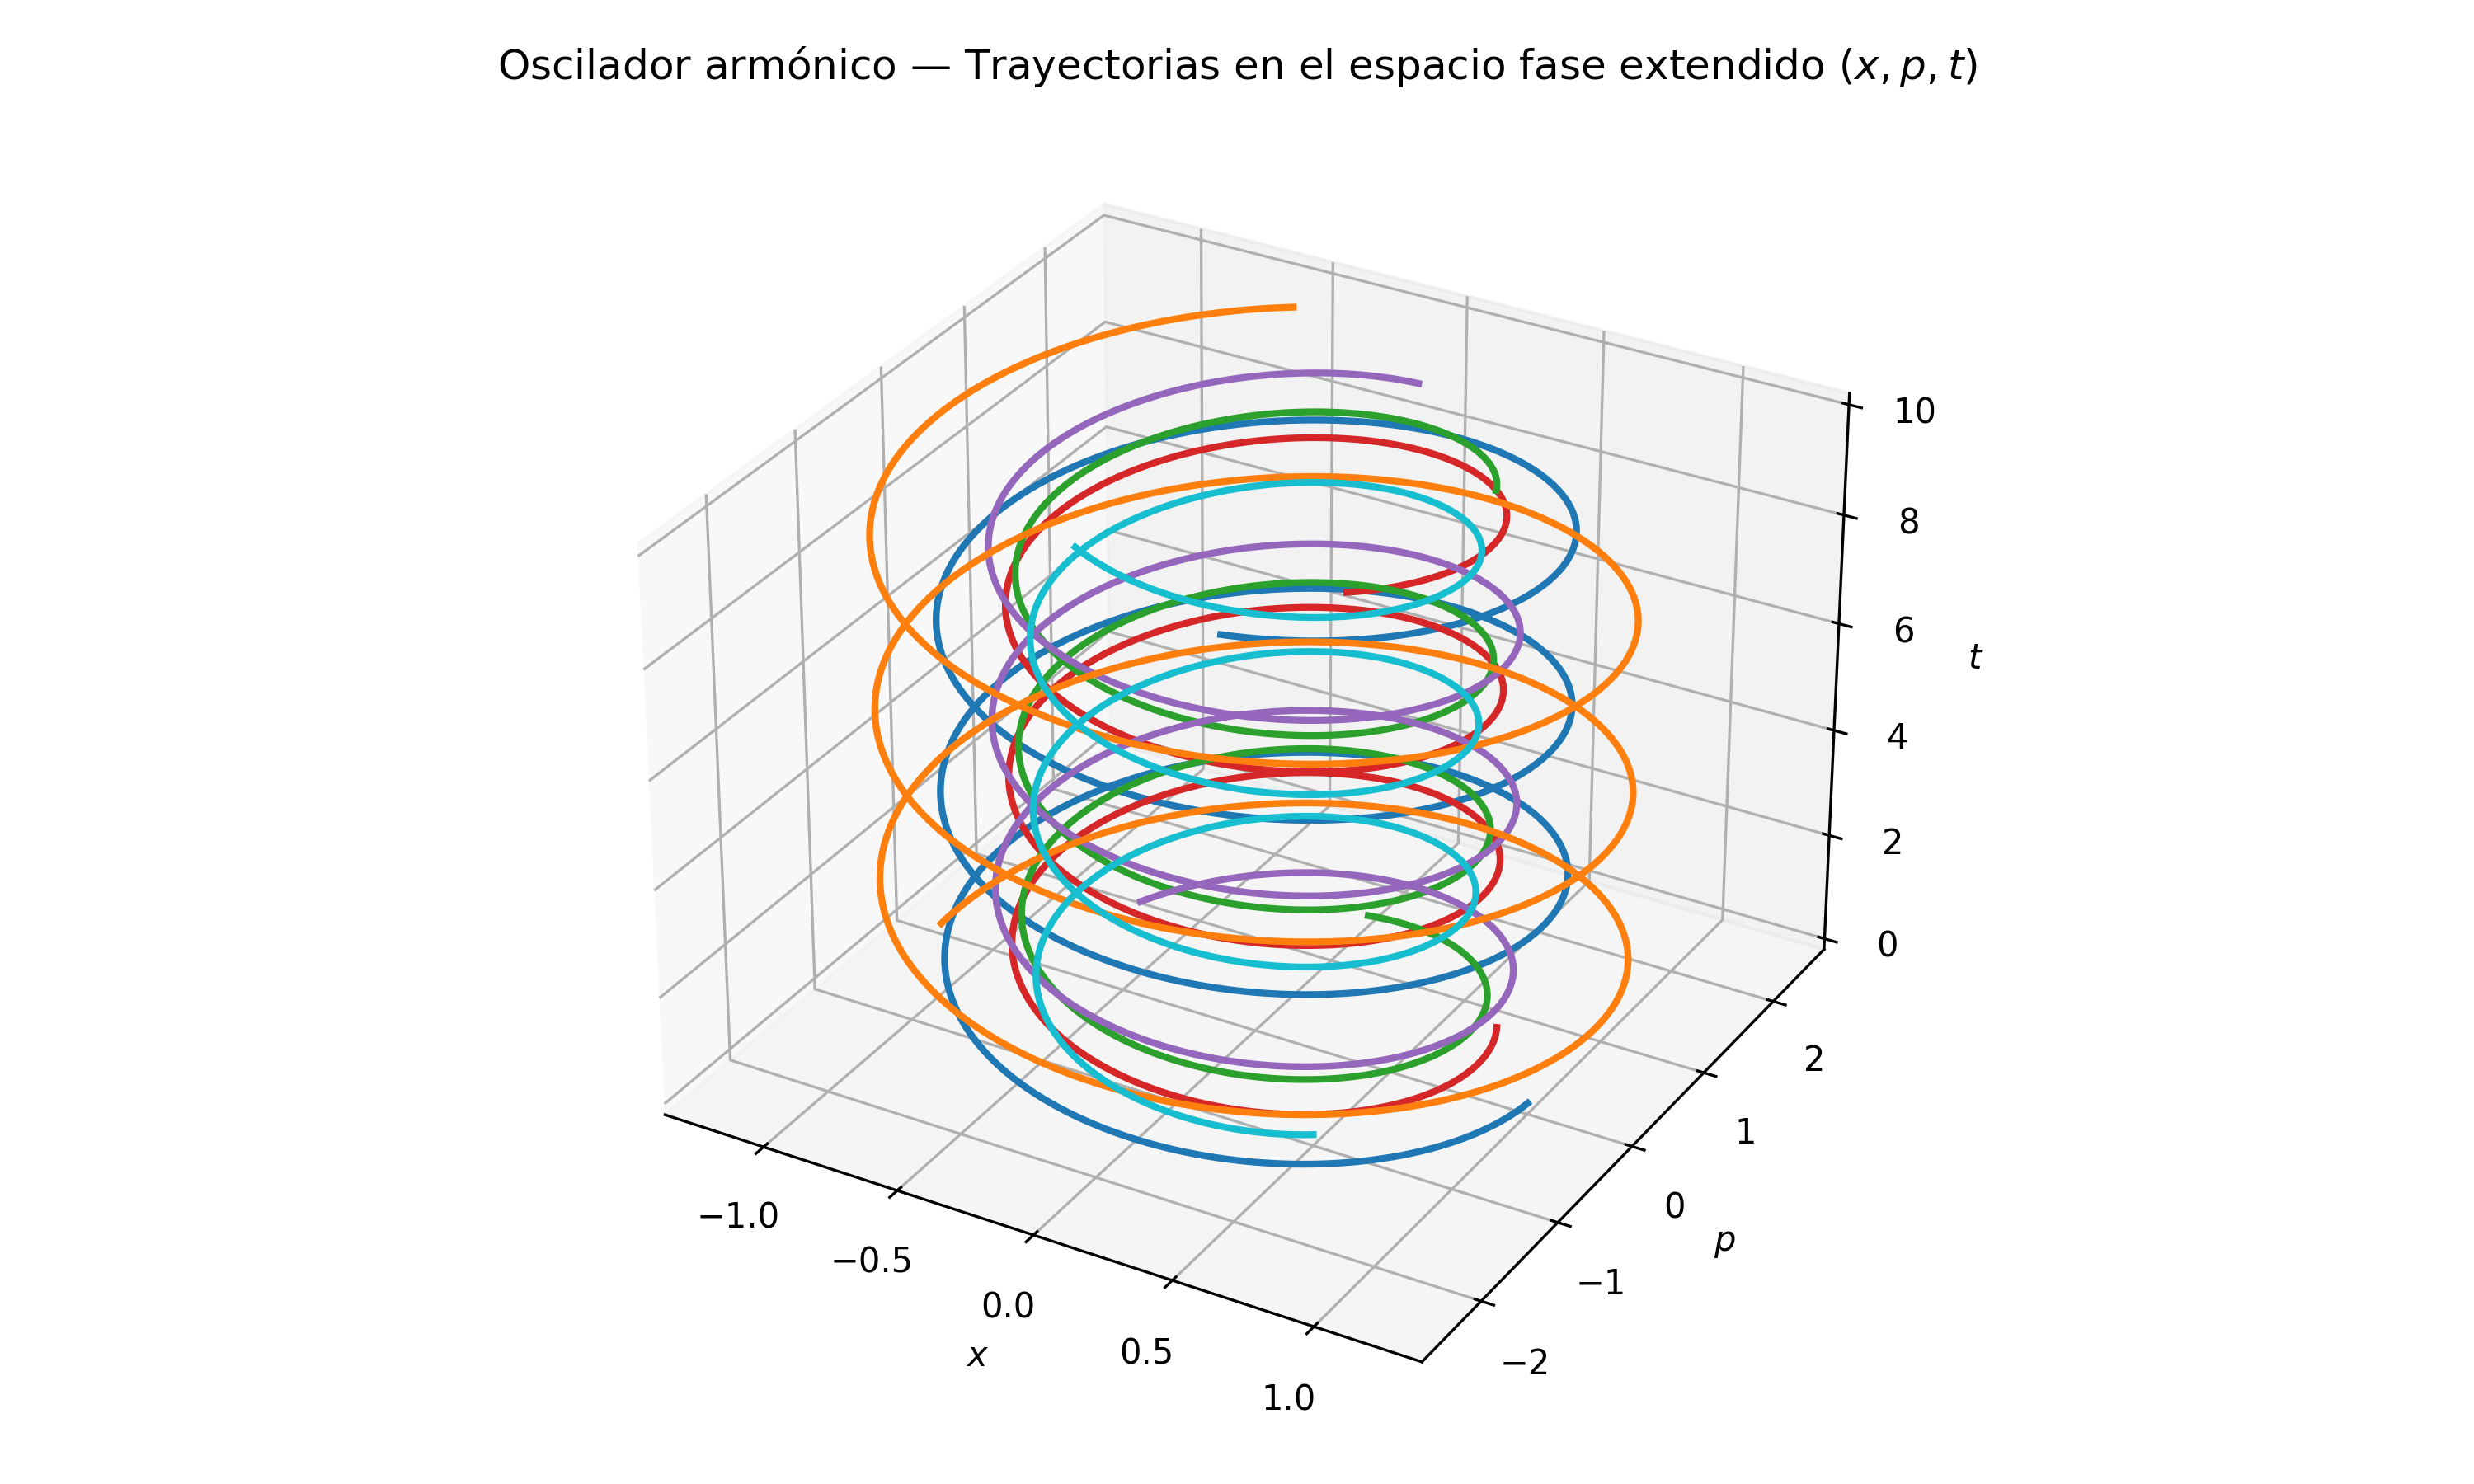
\includegraphics[width=1.1\textwidth]{oscilador_xpt.png}
\caption{
Trayectorias del oscilador armónico simple en el \textbf{espacio fase extendido}
\((x,p,t)\) para distintos valores de \((x_{0},p_{0})\).  
Cada curva es una hélice que asciende en la dirección del tiempo $t$ mientras
su proyección sobre el plano \((x,p)\) recorre la elipse correspondiente a una
energía fija.  
La gráfica fue generada en \texttt{Python} con \texttt{matplotlib} (modo 3D),
utilizando \(m=1\), \(\omega=1\) y las mismas condiciones iniciales que en la
Figura~\ref{fig:oscilador-xp}.}
\label{fig:oscilador-xpt}
\end{figure}



\begin{AGbox}[8]
\begin{enumerate}[label={{\textcolor{trueblue}{\textbf{Pr.} 4.3}}}]
  \item Obtener el Lagrangiano, el Hamiltoniano y las ecuaciones de Hamilton para el problema del plano inclinado.
\end{enumerate}
\end{AGbox}
\vspace{0.5cm}


\textcolor{Cinnabar}{\textbf{Solución:}} \vspace{0.5cm}

\begin{figure}[H]
\centering
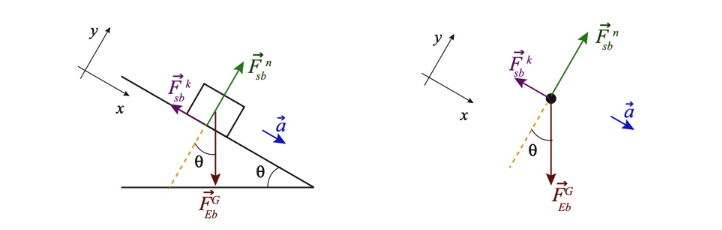
\includegraphics[width=0.75\textwidth]{plano_inclinado.png}
\caption{\textbf{Plano inclinado}. A la izquierda se muestra un bloque de masa $m$
sobre un plano que forma un ángulo $\theta$ con la horizontal; actúan el peso
$\vec F^{G}_{\text{Eb}}$, la reacción normal $\vec F^{n}_{\text{sb}}$ y, en caso de
haber rozamiento, la fuerza de fricción $\vec F^{k}_{\text{sb}}$. A la derecha se
representa el mismo sistema idealizado como una partícula que se desliza a lo largo
de la recta del plano con aceleración $\vec a$}
\label{fig:plano-inclinado}
\end{figure}

Antes de escribir el Lagrangiano y el Hamiltoniano, conviene identificar claramente
el \textbf{número de grados de libertad} del sistema.  
En general, un sistema de \(N\) partículas en el espacio tridimensional requiere
\(3N\) coordenadas para especificar una configuración arbitraria. Si además
existen \(\mathcal{K}\) restricciones holonómicas independientes,
\[
f_{a}(x_{1},y_{1},z_{1},\dots,x_{N},y_{N},z_{N},t)=0,
\qquad a=1,\dots,\mathcal{K}
\]
el número de grados de libertad queda reducido a
\[
n = 3N - \mathcal{K}
\]

En el problema del plano inclinado consideramos una sola partícula (el bloque)
de masa \(m\), así que \(N=1\) y, en ausencia de restricciones, tendríamos tres
coordenadas cartesianas \((x,y,z)\).  
Sin embargo, la situación física mostrada en la
Figura~\ref{fig:plano-inclinado} impone dos restricciones holonómicas:

\begin{itemize}
  \item[$\bullet$] El movimiento ocurre en el \textbf{plano \(x\!-\!y\)}, que podemos
  identificar con la restricción
  \[
    z = 0.
  \]

  \item[$\bullet$] Dentro de ese plano, la partícula está confinada a la
  \textbf{recta del plano inclinado}.  
  En coordenadas \((x,y)\), la ecuación general de una recta es
  \[
     y - y_{0} = m(x - x_{0}),
  \]
  donde la pendiente es \(m = \tan\theta\).  
  Elegimos el punto \((x_{0},y_{0})=(0,0)\) como origen de la recta para simplificar
  la descripción geométrica: cualquier otra elección sólo desplaza la recta en el
  plano y añade constantes que no modifican la física ni las ecuaciones de movimiento
  (pues los potenciales están definidos salvo una constante aditiva).  
  Con esta elección, la restricción adopta su forma más simple,
  \[
    y - x\tan\theta = 0,
  \]
  lo que permite parametrizar el movimiento del bloque usando una única coordenada
  a lo largo del plano inclinado.
\end{itemize}

De esta forma tenemos \(\mathcal{K}=2\) restricciones independientes y el número
de grados de libertad queda
\[
n = 3N - \mathcal{K} = 3 - 2 = 1.
\]


Es decir, \textbf{sólo un parámetro escalar} es suficiente para describir la
configuración del sistema en todo instante.  
Resulta natural escoger como coordenada generalizada \(q\) la \emph{distancia
medida a lo largo del plano} desde un origen conveniente (por ejemplo, desde el
punto más bajo del plano).  

Además, para obtener un Lagrangiano y un Hamiltoniano sencillos consideraremos un
\textbf{plano liso}, es decir, sin rozamiento. En este caso la reacción normal
\(\vec F^{n}_{\text{sb}}\) únicamente asegura la restricción geométrica, pero no
realiza trabajo sobre la partícula, y la única fuerza que contribuye al potencial
es el peso \(\vec F^{G}_{\text{Eb}}\).

\vspace{0.5cm}
\textbf{Descripción geométrica y energía cinética}

Tomamos un sistema de referencia inercial con eje horizontal \(X\) y eje vertical
\(Y\) apuntando hacia arriba. El plano inclinado forma un ángulo \(\theta\) con la
horizontal. Si \(q\) mide la distancia del bloque a lo largo del plano, el vector
de posición de la masa puede escribirse como

\begin{equation}
\begin{split}
\vec r(q)
&= X\,\hat e_{X} + Y\,\hat e_{Y} \\[4pt]
&= q\cos\theta\,\hat e_{X}
 \;+\; q\sin\theta\,\hat e_{Y}
\end{split}\label{eq:posicion-plano-inclinado}
\end{equation}

La velocidad se obtiene derivando \eqref{eq:posicion-plano-inclinado} respecto al
tiempo,

\begin{equation}
\begin{split}
\dot{\vec r}(q)
&= \dot q\cos\theta\,\hat e_{X}
 \;+\; \dot q\sin\theta\,\hat e_{Y}
\end{split}\label{eq:velocidad-plano-inclinado}
\end{equation}

y su módulo al cuadrado es simplemente

\begin{equation}
\begin{split}
v^{2}
&= \dot q^{2}\cos^{2}\theta + \dot q^{2}\sin^{2}\theta \\[4pt]
&= \dot q^{2}\bigl(\cos^{2}\theta+\sin^{2}\theta\bigr) \\[4pt]
&= \dot q^{2}
\end{split}\label{eq:rapidez-plano-inclinado}
\end{equation}

Por lo tanto, la energía cinética del bloque en el plano inclinado es

\begin{equation}
\begin{split}
T &= \frac{1}{2}m v^{2}
   = \frac{1}{2}m\dot q^{2}
\end{split}\label{eq:T-plano-inclinado}
\end{equation}

\vspace{0.5cm}
\textbf{Energía potencial gravitacional}

La altura del bloque sobre el origen vertical (tomando \(Y=0\) en la base del plano)
está dada por \(Y = q\sin\theta\).  
La energía potencial gravitacional, con el cero elegido en el nivel \(Y=0\), es

\begin{equation}
\begin{split}
U(q) &= m g Y = m g\,q\sin\theta
\end{split}\label{eq:U-plano-inclinado}
\end{equation}

De esta manera, cuando el bloque sube por el plano (\(q\) aumenta), también aumenta
su energía potencial; cuando desciende, \(U\) disminuye.

\vspace{0.5cm}
\textbf{Lagrangiano del plano inclinado}

El Lagrangiano es la diferencia entre energía cinética y potencial,

\begin{equation}
\begin{split}
L(q,\dot q)
&= T - U \\[4pt]
&= \frac{1}{2}m\dot q^{2} - m g\,q\sin\theta
\end{split}\label{eq:L-plano-inclinado}
\end{equation}

Esta expresión muestra que el único grado de libertad \(q\) se mueve de forma
efectiva en un potencial lineal \(-m g q\sin\theta\) a lo largo del plano.

\vspace{0.5cm}
\textbf{Momento generalizado y espacio fase}

La coordenada generalizada es simplemente \(q\).  
El momento canónico asociado se define como

\begin{equation}
\begin{split}
p &\equiv \frac{\partial L}{\partial\dot q}
       = m\dot q
\end{split}\label{eq:momento-plano-inclinado}
\end{equation}

De aquí podemos invertir para escribir la “velocidad” \(\dot q\) en términos del
momento,

\begin{equation}
\begin{split}
\dot q &= \frac{p}{m}
\end{split}\label{eq:velocidad-en-funcion-de-p}
\end{equation}

De este modo, el \textbf{espacio fase} del sistema está parametrizado por el par
\((q,p)\).

\vspace{0.5cm}
\textbf{Hamiltoniano del plano inclinado}

El Hamiltoniano se obtiene como transformada de Legendre del Lagrangiano
\eqref{eq:L-plano-inclinado} con respecto a la velocidad \(\dot q\),

\[
H(q,p) \equiv p\dot q - L
\]

Sustituyendo \eqref{eq:velocidad-en-funcion-de-p} y la expresión
\eqref{eq:L-plano-inclinado}, se puede reescribir \(H\) en términos de \(q\) y \(p\)
únicamente. Primero expresamos la energía cinética en función de \(p\),

\begin{equation}
\begin{split}
T &= \frac{1}{2}m\dot q^{2}
   = \frac{1}{2}m\left(\frac{p}{m}\right)^{2}
   = \frac{p^{2}}{2m}
\end{split}\label{eq:T-en-p-plano-inclinado}
\end{equation}

Luego, como \(L = T - U\), la transformada de Legendre nos lleva a

\begin{equation}
\begin{split}
H(q,p)
&= T + U \\[4pt]
&= \frac{p^{2}}{2m} + m g\,q\sin\theta
\end{split}\label{eq:H-plano-inclinado}
\end{equation}

El Hamiltoniano \eqref{eq:H-plano-inclinado} coincide con la energía total del
sistema (suma de energía cinética y potencial) y, como no depende explícitamente del
tiempo, es una \textbf{constante de movimiento}.

\vspace{0.5cm}
\textbf{Ecuaciones de Hamilton}

Las ecuaciones de Hamilton para un sistema de un solo grado de libertad se escriben
como

\[
\dot q = \frac{\partial H}{\partial p},
\qquad
\dot p = -\,\frac{\partial H}{\partial q}
\]

A partir del Hamiltoniano \eqref{eq:H-plano-inclinado}, obtenemos

\begin{equation}
\begin{split}
\dot q &= \frac{\partial H}{\partial p}
       = \frac{p}{m} \\[4pt]
\dot p &= -\,\frac{\partial H}{\partial q}
       = -\,m g\sin\theta
\end{split}\label{eq:ecuaciones-H-plano-inclinado}
\end{equation}

La primera ecuación de \eqref{eq:ecuaciones-H-plano-inclinado} no es otra cosa que
la relación ya conocida entre momento lineal y velocidad en
\eqref{eq:velocidad-en-funcion-de-p}.  
La segunda ecuación indica que la derivada temporal del momento es constante e igual
a \(-m g\sin\theta\), lo cual se traduce en una aceleración constante a lo largo
del plano.

Si derivamos nuevamente \(\dot q\) respecto al tiempo y usamos \(\dot p\) obtenida en
\eqref{eq:ecuaciones-H-plano-inclinado}, recuperamos la ecuación de movimiento de
segundo orden,

\begin{equation}
\begin{split}
\ddot q
&= \frac{1}{m}\dot p
 = -\,g\sin\theta
\end{split}\label{eq:ecuacion-segundo-orden-plano}
\end{equation}

Esta ecuación diferencial de segundo orden \eqref{eq:ecuacion-segundo-orden-plano}
es, en sentido estricto, \textbf{la ecuación de movimiento} del sistema.
Recordemos que, tras el análisis de grados de libertad,
\[
n = 3N - \mathcal{K} = 3 - 2 = 1,
\]
concluimos que el sistema posee un solo parámetro independiente \(q(t)\).
Por tanto, \emph{toda la dinámica} del bloque sobre el plano debe quedar codificada
en una única ecuación diferencial de segundo orden para \(q(t)\), y ésta es
precisamente
\[
\ddot q = -\,g\sin\theta.
\]

Además, esta forma coincide exactamente con la aceleración física del bloque
obtenida mediante el tratamiento newtoniano del plano inclinado sin fricción:
la componente del peso paralela al plano es \(-mg\sin\theta\), lo cual conduce a
la misma ecuación de movimiento. De este modo, el formalismo lagrangiano–hamiltoniano
recupera de manera elegante y sistemática la dinámica esperada.


\vspace{0.4cm}

El problema del plano inclinado con plano liso y bloque de masa
\(m\) se reduce, en la formulación lagrangiana y hamiltoniana, a un sistema de un
solo grado de libertad descrito por el Hamiltoniano

\begin{equation}
\begin{split}
H(q,p)
&= \frac{p^{2}}{2m} + m g\,q\sin\theta
\end{split}\label{eq:H-plano-inclinado-resumen}
\end{equation}

y las ecuaciones de Hamilton \eqref{eq:ecuaciones-H-plano-inclinado}, que codifican
que el bloque se mueve con aceleración constante \(-g\sin\theta\) a lo largo del
plano, en completo acuerdo con la descripción elemental del plano inclinado, pero
ahora vista desde la perspectiva elegante del formalismo de Hamilton.

Aunque el problema no lo solicita, podemos integrar explícitamente la ecuación
de movimiento \(\ddot q = -g\sin\theta\) para obtener las soluciones cerradas del
movimiento. Integrando una vez:

\[
\dot q(t) = \dot q_0 - g\sin\theta\, t,
\]

y volviendo a integrar:

\[
q(t) = q_0 + \dot q_0 t - \frac{1}{2}g\sin\theta\, t^{2}.
\]

Como el momento es \(p = m\dot q\), obtenemos también

\[
p(t) = p_0 - m g\sin\theta\, t.
\]

Estas soluciones muestran explícitamente la caída uniforme del bloque a lo largo
del plano e ilustran cómo el formalismo hamiltoniano recupera la dinámica esperada,
pero se incluyen únicamente como observación complementaria.
\vspace{0.4cm}

El problema del plano inclinado con plano liso y bloque de masa
\(m\) se reduce, en la formulación lagrangiana y hamiltoniana, a un sistema de un
solo grado de libertad descrito por el Hamiltoniano

\begin{equation}
\begin{split}
H(q,p)
&= \frac{p^{2}}{2m} + m g\,q\sin\theta
\end{split}\label{eq:H-plano-inclinado-resumen}
\end{equation}

y las ecuaciones de Hamilton \eqref{eq:ecuaciones-H-plano-inclinado}, que codifican
que el bloque se mueve con aceleración constante \(-g\sin\theta\) a lo largo del
plano, en completo acuerdo con la descripción elemental del plano inclinado, pero
ahora vista desde la perspectiva elegante del formalismo de Hamilton.

\vspace{0.5cm}


%=============================
% PR. 4.4
%=============================

\begin{AGbox}[8]
\begin{enumerate}[label={{\textcolor{trueblue}{\textbf{Pr.} 4.4}}}]
  \item El Lagrangiano del oscilador armónico isotrópo en dos dimensiones está dado por
  \begin{equation}
  \begin{split}
  L(x,y,\dot{x},\dot{y})
  &= \frac{m}{2}\bigl(\dot{x}^{2} + \dot{y}^{2}\bigr)
     - \frac{m\omega^{2}}{2}\bigl(x^{2} + y^{2}\bigr)
  \end{split}
  \label{eq:L-2D-isotropo}
  \end{equation}
  Obtener las ecuaciones de Hamilton, resolverlas y presentar en un solo gráfico
  algunas trayectorias, para diferentes condiciones iniciales, en el espacio de
  configuraciones
\end{enumerate}
\end{AGbox}
\vspace{0.5cm}

\textcolor{Cinnabar}{\textbf{Solución:}} \vspace{0.4cm}

La fucncion Lagrangiana de la ecuación (\underline{enunciado}) \eqref{eq:L-2D-isotropo} describe a una partícula de masa $m$
moviéndose en el plano $(x,y)$ bajo un potencial armónico \emph{isotrópo}, es
decir, con la misma frecuencia angular $\omega$ en todas las direcciones.
El término cinético es proporcional a $\dot{x}^{2}+\dot{y}^{2}$ y el potencial
depende únicamente de la distancia al origen
\begin{equation}
r^{2} = x^{2} + y^{2}
\label{eq:r-cuadrado}
\end{equation}
lo que hace explícita la simetría circular del problema

%------------------------------------------------
\textcolor{trueblue}{\textbf{Calculamos los omentos generalizados y la función hamiltoniana}}
%------------------------------------------------

A partir de \eqref{eq:L-2D-isotropo} obtenemos los momentos canónicos conjugados
a las coordenadas generalizadas $x$ e $y$ mediante las definiciones habituales
\begin{equation}
\begin{split}
p_{x} &\equiv \frac{\partial L}{\partial \dot{x}} \\[4pt]
p_{y} &\equiv \frac{\partial L}{\partial \dot{y}}
\end{split}
\label{eq:def-momenta-2D}
\end{equation}

Sustituyendo \eqref{eq:L-2D-isotropo} en \eqref{eq:def-momenta-2D} se obtiene
\begin{equation}
\begin{split}
p_{x} &= m\,\dot{x} \\[4pt]
p_{y} &= m\,\dot{y}
\end{split}
\label{eq:px-py-2D}
\end{equation}

Las relaciones \eqref{eq:px-py-2D} se pueden invertir para expresar las
velocidades en términos de los momentos
\begin{equation}
\begin{split}
\dot{x} &= \frac{p_{x}}{m} \\[4pt]
\dot{y} &= \frac{p_{y}}{m}
\end{split}
\label{eq:xdot-ydot-2D}
\end{equation}

La Hamiltoniana se define mediante la \textbf{transformación de Legendre} que hemos estado trabajando continuamente en el edsarrollo de los ejercicios
\begin{equation}
\begin{split}
H(x,y,p_{x},p_{y})
&\equiv p_{x}\dot{x} + p_{y}\dot{y} - L(x,y,\dot{x},\dot{y})
\end{split}
\label{eq:H-def-2D}
\end{equation}
donde en \eqref{eq:H-def-2D} debe entenderse que $\dot{x}$ y $\dot{y}$ se
sustituyen por las expresiones \eqref{eq:xdot-ydot-2D}

Sustituyendo \eqref{eq:xdot-ydot-2D} y \eqref{eq:L-2D-isotropo} en
\eqref{eq:H-def-2D} se llega a
\begin{equation}
\begin{split}
H(x,y,p_{x},p_{y})
&= p_{x}\left(\frac{p_{x}}{m}\right)
   + p_{y}\left(\frac{p_{y}}{m}\right) \\[4pt]
&\quad
   - \frac{m}{2}\left[
      \left(\frac{p_{x}}{m}\right)^{2}
      + \left(\frac{p_{y}}{m}\right)^{2}
     \right]
   + \frac{m\omega^{2}}{2}\bigl(x^{2}+y^{2}\bigr)
\end{split}
\label{eq:H-2D-paso-intermedio}
\end{equation}

Tras simplificar los factores,
\begin{equation}
\begin{split}
H(x,y,p_{x},p_{y})
&= \frac{p_{x}^{2}+p_{y}^{2}}{2m}
   + \frac{m\omega^{2}}{2}\bigl(x^{2}+y^{2}\bigr)
\end{split}
\label{eq:H-2D-oscilador}
\end{equation}

La expresión \eqref{eq:H-2D-oscilador} muestra con claridad que la energía
total se descompone en
\begin{equation}
\begin{split}
T &= \frac{p_{x}^{2}+p_{y}^{2}}{2m} \\[4pt]
V &= \frac{m\omega^{2}}{2}\bigl(x^{2}+y^{2}\bigr)
\end{split}
\label{eq:T-V-2D}
\end{equation}
es decir, energía cinética más energía potencial armónica isotrópa

%------------------------------------------------
\textcolor{trueblue}{\textbf{Ecuaciones de Hamilton}}
%------------------------------------------------

Las ecuaciones de Hamilton para este sistema de dos grados de libertad se
escriben, en general, como
\begin{equation}
\begin{split}
\dot{x} &= \frac{\partial H}{\partial p_{x}} \\[4pt]
\dot{y} &= \frac{\partial H}{\partial p_{y}} \\[4pt]
\dot{p}_{x} &= -\,\frac{\partial H}{\partial x} \\[4pt]
\dot{p}_{y} &= -\,\frac{\partial H}{\partial y}
\end{split}
\label{eq:hamilton-2D-general}
\end{equation}

Aplicando \eqref{eq:hamilton-2D-general} al Hamiltoniano
\eqref{eq:H-2D-oscilador}, es decir,
\[
H(x,y,p_{x},p_{y})
= \frac{p_{x}^{2}+p_{y}^{2}}{2m}
  + \frac{m\omega^{2}}{2}\bigl(x^{2}+y^{2}\bigr)
\]
obtenemos, componente por componente,
\begin{equation}
\begin{split}
\dot{x} &=
\frac{\partial}{\partial p_{x}}
\left[
  \frac{p_{x}^{2}+p_{y}^{2}}{2m}
  + \frac{m\omega^{2}}{2}\bigl(x^{2}+y^{2}\bigr)
\right]
= \frac{p_{x}}{m} \\[6pt]
\dot{y} &=
\frac{\partial}{\partial p_{y}}
\left[
  \frac{p_{x}^{2}+p_{y}^{2}}{2m}
  + \frac{m\omega^{2}}{2}\bigl(x^{2}+y^{2}\bigr)
\right]
= \frac{p_{y}}{m} \\[6pt]
\dot{p}_{x} &=
-\,\frac{\partial}{\partial x}
\left[
  \frac{p_{x}^{2}+p_{y}^{2}}{2m}
  + \frac{m\omega^{2}}{2}\bigl(x^{2}+y^{2}\bigr)
\right]
= -\,m\omega^{2}x \\[6pt]
\dot{p}_{y} &=
-\,\frac{\partial}{\partial y}
\left[
  \frac{p_{x}^{2}+p_{y}^{2}}{2m}
  + \frac{m\omega^{2}}{2}\bigl(x^{2}+y^{2}\bigr)
\right]
= -\,m\omega^{2}y
\end{split}
\label{eq:hamilton-2D-oscilador}
\end{equation}

El sistema \eqref{eq:hamilton-2D-oscilador} se separa en dos pares de ecuaciones
idénticas, uno para el par $(x,p_{x})$ y otro para el par $(y,p_{y})$. Si
derivamos de nuevo las dos primeras ecuaciones de
\eqref{eq:hamilton-2D-oscilador} y sustituimos las últimas dos, obtenemos
\begin{equation}
\begin{split}
\ddot{x} &= \frac{\dot{p}_{x}}{m}
         = -\,\omega^{2}x \\[4pt]
\ddot{y} &= \frac{\dot{p}_{y}}{m}
         = -\,\omega^{2}y
\end{split}
\label{eq:edo-2D-oscilador}
\end{equation}
es decir, cada coordenada cumple la ecuación del oscilador armónico simple
de frecuencia $\omega$.

%------------------------------------------------
\textcolor{trueblue}{\textbf{Formulación matricial del oscilador isotrópo en 2D}}
%------------------------------------------------

La estructura de \eqref{eq:hamilton-2D-oscilador} sugiere una descripción más
compacta en términos de matrices, totalmente análoga al caso unidimensional.
Para ello introducimos el \textbf{vector de fase} de dimensión cuatro
\begin{equation}
\mathbf{Z}(t) \equiv
\begin{pmatrix}
x(t) \\[4pt]
y(t) \\[4pt]
p_{x}(t) \\[4pt]
p_{y}(t)
\end{pmatrix}
\label{eq:vector-fase-2D}
\end{equation}

En términos de \eqref{eq:vector-fase-2D}, el sistema de Hamilton
\eqref{eq:hamilton-2D-oscilador} se puede escribir como una ecuación diferencial
lineal de primer orden
\begin{equation}
\dot{\mathbf{Z}}(t) = M\,\mathbf{Z}(t)
\label{eq:sistema-matricial-2D}
\end{equation}
donde la matriz de coeficientes $4\times 4$ es
\begin{equation}
M =
\begin{pmatrix}
0       & 0       & \dfrac{1}{m} & 0 \\[6pt]
0       & 0       & 0            & \dfrac{1}{m} \\[6pt]
-\,m\omega^{2} & 0 & 0           & 0 \\[6pt]
0       & -\,m\omega^{2} & 0     & 0
\end{pmatrix}
\label{eq:matriz-M-2D}
\end{equation}

Cada fila de \eqref{eq:matriz-M-2D} reproduce, de manera explícita, una de las
ecuaciones de Hamilton:

\begin{itemize}
  \item[$\bullet$] La primera fila noos da la ecuación
  $\dot{x} = p_{x}/m$  
  \item[$\bullet$] La segunda fila nos da la ecuación
  $\dot{y} = p_{y}/m$  
  \item[$\bullet$] La tercera fila nos da la ecuación
  $\dot{p}_{x} = -\,m\omega^{2}x$  
  \item[$\bullet$] La cuarta fila nos da la ecuación
  $\dot{p}_{y} = -\,m\omega^{2}y$
\end{itemize}

Así, la dinámica completa del oscilador armónico isotrópo en dos dimensiones
queda contenida en la ecuación matricial compacta \eqref{eq:sistema-matricial-2D}.

%------------------------------------------------
\textcolor{trueblue}{\textbf{Desacoplo en dos osciladores unidimensionales}}
%------------------------------------------------

La forma de \eqref{eq:matriz-M-2D} muestra que las parejas $(x,p_{x})$ y
$(y,p_{y})$ no se acoplan entre sí. Para hacer esta separación aún más
transparente, reordenamos las componentes del vector de fase y definimos
\begin{equation}
\widetilde{\mathbf{Z}}(t) \equiv
\begin{pmatrix}
x(t) \\[4pt]
p_{x}(t) \\[4pt]
y(t) \\[4pt]
p_{y}(t)
\end{pmatrix}
\label{eq:vector-fase-2D-ordenado}
\end{equation}

La relación entre $\mathbf{Z}(t)$ y $\widetilde{\mathbf{Z}}(t)$ es simplemente
un reordenamiento de componentes, que puede escribirse mediante una matriz de
permutación $P$ tal que
\begin{equation}
\widetilde{\mathbf{Z}}(t) = P\,\mathbf{Z}(t),
\qquad
\mathbf{Z}(t) = P^{-1}\,\widetilde{\mathbf{Z}}(t)
\label{eq:perm-2D}
\end{equation}

En esta nueva base, la ecuación \eqref{eq:sistema-matricial-2D} se transforma en
\begin{equation}
\dot{\widetilde{\mathbf{Z}}}(t)
=
\widetilde{M}\,\widetilde{\mathbf{Z}}(t),
\qquad
\widetilde{M} \equiv P M P^{-1}
\label{eq:sistema-matricial-2D-tilde}
\end{equation}
donde $\widetilde{M}$ adopta una forma de bloques diagonal
\begin{equation}
\widetilde{M} =
\begin{pmatrix}
A & 0 \\[4pt]
0 & A
\end{pmatrix}
\label{eq:M-tilde-bloques}
\end{equation}

Aquí $A$ es exactamente la matriz $2\times 2$ del oscilador armónico
unidimensional estudiado en el problema anterior, ahora destacada en el contexto
bidimensional:
\begin{equation}
A =
\begin{pmatrix}
0 & \dfrac{1}{m} \\[6pt]
-\,m\omega^{2} & 0
\end{pmatrix}
\label{eq:matriz-A-oscilador-2D}
\end{equation}

La ecuación \eqref{eq:M-tilde-bloques} expresa de forma clara que el oscilador
isotrópo en 2D es, desde el punto de vista matricial, la suma directa de dos
copias del oscilador armónico simple unidimensional: una actuando sobre el par
$(x,p_{x})$ y la otra sobre el par $(y,p_{y})$.

%------------------------------------------------
\textcolor{trueblue}{\textbf{Exponencial matricial en dimensión cuatro}}
%------------------------------------------------

El sistema lineal homogéneo \eqref{eq:sistema-matricial-2D-tilde} tiene como
solución formal
\begin{equation}
\widetilde{\mathbf{Z}}(t)
=
e^{\widetilde{M}t}\,\widetilde{\mathbf{Z}}_{0}
\label{eq:solucion-formal-2D-tilde}
\end{equation}
donde
\[
\widetilde{\mathbf{Z}}_{0} =
\begin{pmatrix}
x_{0} \\[2pt]
p_{x0} \\[2pt]
y_{0} \\[2pt]
p_{y0}
\end{pmatrix}
\]
es el estado inicial en la base reordenada. Como $\widetilde{M}$ es diagonal por
bloques, su exponencial se calcula bloque a bloque:
\begin{equation}
e^{\widetilde{M}t}
=
\begin{pmatrix}
e^{At} & 0 \\[4pt]
0      & e^{At}
\end{pmatrix}
\label{eq:exp-M-tilde}
\end{equation}

Por otra parte, en el caso unidimensional ya demostramos que la exponencial
matricial de $A$ se puede escribir en términos de funciones trigonométricas como
\begin{equation}
e^{At} = I\cos(\omega t) + \frac{A}{\omega}\,\sin(\omega t)
\label{eq:exp-At-2D}
\end{equation}
donde $I$ es la matriz identidad $2\times 2$. Sustituyendo
\eqref{eq:exp-At-2D} en \eqref{eq:exp-M-tilde}, la solución formal
\eqref{eq:solucion-formal-2D-tilde} toma la forma explícita
\begin{equation}
\widetilde{\mathbf{Z}}(t)
=
\begin{pmatrix}
e^{At} & 0 \\[4pt]
0      & e^{At}
\end{pmatrix}
\begin{pmatrix}
x_{0}   \\[2pt]
p_{x0}  \\[2pt]
y_{0}   \\[2pt]
p_{y0}
\end{pmatrix}
\label{eq:solucion-formal-2D-tilde-2}
\end{equation}
lo que muestra que el par $(x(t),p_{x}(t))$ evoluciona bajo $e^{At}$ exactamente
igual que en el oscilador de una dimensión, y el par $(y(t),p_{y}(t))$ evoluciona
de manera independiente bajo la misma matriz $e^{At}$.

Finalmente, para regresar a la base original usamos \eqref{eq:perm-2D}. La
solución en términos de $\mathbf{Z}(t)$ se escribe como
\begin{equation}
\mathbf{Z}(t)
=
P^{-1}\,\widetilde{\mathbf{Z}}(t)
=
P^{-1}\,
\begin{pmatrix}
e^{At} & 0 \\[4pt]
0      & e^{At}
\end{pmatrix}
P\,\mathbf{Z}_{0}
\label{eq:solucion-formal-2D-original}
\end{equation}
donde $\mathbf{Z}_{0} = (x_{0},y_{0},p_{x0},p_{y0})^{T}$ es el vector de fase
inicial en el orden original de componentes.

Desde el punto de vista físico, \eqref{eq:solucion-formal-2D-original} hace
explícito que el oscilador armónico isotrópo en dos dimensiones se comporta
como dos osciladores armónicos independientes de igual frecuencia $\omega$,
acoplados únicamente a través de la energía total y de la simetría de rotación
del potencial.

\bigskip
\textcolor{trueblue}{\textbf{Soluciones para $x(t)$, $y(t)$ y momentos canónicos}}
%------------------------------------------------

La solución general de \eqref{eq:edo-2D-oscilador} se escribe en términos de
funciones seno y coseno. Usando las condiciones iniciales
\begin{equation}
\begin{split}
x(0) &= x_{0},
\qquad
\dot{x}(0) = v_{x0} \\[4pt]
y(0) &= y_{0},
\qquad
\dot{y}(0) = v_{y0}
\end{split}
\label{eq:condiciones-iniciales-2D}
\end{equation}
se obtiene
\begin{equation}
\begin{split}
x(t) &= x_{0}\cos(\omega t)
     + \frac{v_{x0}}{\omega}\,\sin(\omega t) \\[4pt]
y(t) &= y_{0}\cos(\omega t)
     + \frac{v_{y0}}{\omega}\,\sin(\omega t)
\end{split}
\label{eq:x-y-sol-2D}
\end{equation}

A partir de \eqref{eq:px-py-2D} y \eqref{eq:x-y-sol-2D} se calculan los momentos
canónicos
\begin{equation}
\begin{split}
p_{x}(t)
&= m\,\dot{x}(t)
 = m\left[
     -\,\omega x_{0}\sin(\omega t)
     + v_{x0}\cos(\omega t)
   \right] \\[6pt]
p_{y}(t)
&= m\,\dot{y}(t)
 = m\left[
     -\,\omega y_{0}\sin(\omega t)
     + v_{y0}\cos(\omega t)
   \right]
\end{split}
\label{eq:px-py-sol-2D}
\end{equation}

Las soluciones \eqref{eq:x-y-sol-2D} y \eqref{eq:px-py-sol-2D} satisfacen
directamente el sistema de Hamilton \eqref{eq:hamilton-2D-oscilador} y
conservan la energía \eqref{eq:H-2D-oscilador} para todo $t$. Además, son
consistentes con la solución matricial \eqref{eq:solucion-formal-2D-original},
pues la acción del bloque $e^{At}$ sobre los vectores iniciales
\[
(x_{0},p_{x0})^{T},
\qquad
(y_{0},p_{y0})^{T}
\]
reproduce exactamente las expresiones escalares anteriores.

%------------------------------------------------
\textcolor{trueblue}{\textbf{Trayectorias en el espacio de configuraciones $(x,y)$}}
%------------------------------------------------

El movimiento en el espacio de configuraciones está descrito por la curva
paramétrica
\begin{equation}
\gamma(t) =
\bigl(x(t),y(t)\bigr)
\label{eq:trayectoria-xy}
\end{equation}
donde $x(t)$ e $y(t)$ están dados por \eqref{eq:x-y-sol-2D}. Es útil reescribir
\eqref{eq:x-y-sol-2D} como
\begin{equation}
\begin{split}
x(t) &= A_{x}\cos(\omega t) + B_{x}\sin(\omega t) \\[4pt]
y(t) &= A_{y}\cos(\omega t) + B_{y}\sin(\omega t)
\end{split}
\label{eq:x-y-A-B}
\end{equation}
con
\begin{equation}
\begin{split}
A_{x} &= x_{0},
\qquad
B_{x} = \frac{v_{x0}}{\omega} \\[4pt]
A_{y} &= y_{0},
\qquad
B_{y} = \frac{v_{y0}}{\omega}
\end{split}
\label{eq:A-B-def}
\end{equation}

En forma vectorial, \eqref{eq:x-y-A-B} puede escribirse como
\begin{equation}
\vec r(t)
=
\underbrace{\begin{pmatrix} A_{x} \\[2pt] A_{y} \end{pmatrix}}_{\textcolor{Tarawera}{\vec a}}
\cos(\omega t)
+
\underbrace{\begin{pmatrix} B_{x} \\[2pt] B_{y} \end{pmatrix}}_{\textcolor{Cinnabar}{\vec b}}
\sin(\omega t)
\label{eq:r-A-B}
\end{equation}

La ecuación \eqref{eq:r-A-B} es precisamente el parámetro estándar de una
\textbf{elipse} en el plano $(x,y)$: el punto $\vec r(t)$ se mueve sobre una
elipse con periodo
\begin{equation}
T = \frac{2\pi}{\omega}
\label{eq:periodo-2D}
\end{equation}
recorriéndola indefinidamente sin cambiar su energía

Casos particulares interesantes:

\begin{itemize}
  \item[$\bullet$] Si los vectores $\vec a$ y $\vec b$ en \eqref{eq:r-A-B} son
  ortogonales y tienen la misma norma, la elipse se reduce a una
  \textbf{circunferencia}. Esto se logra, por ejemplo, con
  $x_{0}=R$, $y_{0}=0$, $v_{x0}=0$ y $v_{y0}=R\omega$
  \item[$\bullet$] Si $\vec b$ es proporcional a $\vec a$, la elipse se colapsa
  en un segmento de recta y la partícula oscila sobre un diámetro fijo
\end{itemize}

En todos los casos, las curvas cerradas en el plano $(x,y)$ reflejan tanto la
conservación de la energía \eqref{eq:H-2D-oscilador} como la simetría de rotación
implícita en el potencial \eqref{eq:r-cuadrado}

%------------------------------------------------
\textcolor{trueblue}{\textbf{5) Un solo gráfico con varias trayectorias}}
%------------------------------------------------

Para ilustrar las trayectorias en el espacio de configuraciones se puede usar
\texttt{pgfplots} y representar curvas de la forma \eqref{eq:trayectoria-xy}
para varios conjuntos de condiciones iniciales. Un ejemplo es el siguiente

\begin{figure}[H]
\centering
\begin{tikzpicture}
\begin{axis}[
    xlabel={$x$},
    ylabel={$y$},
    axis equal image,
    grid=both,
    width=11cm,
    height=8cm,
    axis lines=middle,
    clip=false,               % <-- permite que la leyenda salga del cuadro
    legend style={
      font=\footnotesize,
      at={(0.5,1.04)},        % <-- centrada arriba del eje
      anchor=south,
      legend cell align=left
    },
]

% t de 0 a 2*pi (una oscilación completa)
\addplot[domain=0:2*pi,samples=300,very thick,color=trueblue]
  ({cos(deg(x))},
   {sin(deg(x))});
\addlegendentry{$(x_{0},y_{0})=(1,0),\ (v_{x0},v_{y0})=(0,\omega)$}

\addplot[domain=0:2*pi,samples=300,very thick,color=Cinnabar]
  ({1.2*cos(deg(x))},
   {0.6*sin(deg(x))});
\addlegendentry{Elipse $(A_{x},A_{y})=(1.2,0),\ (B_{x},B_{y})=(0,0.6)$}

\addplot[domain=0:2*pi,samples=300,very thick,color=AppleGreen]
  ({0.7*cos(deg(x)) + 0.2*sin(deg(x))},
   {0.2*cos(deg(x)) + 0.9*sin(deg(x))});
\addlegendentry{Elipse general ($\vec a$ y $\vec b$ no ortogonales)}

\end{axis}
\end{tikzpicture}
\caption{
Trayectorias del oscilador armónico isotrópo en el \textbf{espacio de
configuraciones} $(x,y)$, obtenidas a partir de las soluciones
\eqref{eq:x-y-sol-2D} para diferentes condiciones iniciales.  
Cada curva es una elipse (incluyendo el caso particular de circunferencia),
recorrida periódicamente con periodo \eqref{eq:periodo-2D}, lo que refleja la
naturaleza oscilatoria y la simetría de rotación del potencial
$V=\tfrac{1}{2}m\omega^{2}(x^{2}+y^{2})$
}
\label{fig:trayectorias-xy-2D}
\end{figure}



%=============================
% PR. 4.5
%=============================

\begin{AGbox}[8]
\begin{enumerate}[label={{\textcolor{trueblue}{\textbf{Pr.} 4.5}}}]
  \item Hemos mostrado que el Hamiltoniano de una partícula cargada en un campo magnético constante está dado por 
  \[
  H(\mathbf{r},\mathbf{p},t) = \frac{1}{2m}(p_{x}^{2}+p_{y}^{2}+p_{z}^{2}) + \frac{\omega_{0}}{2}(yp_{x}-xp_{y}) + \frac{m\omega_{0}^{2}}{8}(x^{2}+y^{2}).
  \]
  Resolver la ecuaciones de Hamilton y presentar en un solo gráfico algunas trayectorias para diferentes condiciones iniciales en el espacio de configuraciones.
\end{enumerate}
\end{AGbox}
\vspace{0.5cm}

%=============================
% PR. 4.5 — Partícula cargada en B constante
%=============================
\textcolor{Cinnabar}{\textbf{Solución:}} \vspace{0.5cm}

El Hamiltoniano que describe a una partícula cargada en un campo magnético
constante se puede escribir como
\begin{equation}
H(x,y,z,p_{x},p_{y},p_{z})
=
\frac{1}{2m}\bigl(p_{x}^{2}+p_{y}^{2}+p_{z}^{2}\bigr)
+ \frac{\omega_{0}}{2}\bigl(yp_{x}-xp_{y}\bigr)
+ \frac{m\omega_{0}^{2}}{8}\bigl(x^{2}+y^{2}\bigr)
\label{eq:H-magnetico}
\end{equation}
donde $\omega_{0}$ es una constante proporcional a la intensidad del campo
magnético y al cociente carga/masa de la partícula.

%------------------------------------------------
\textcolor{trueblue}{\textbf{Ecuaciones de Hamilton}}
%------------------------------------------------

Aplicamos las ecuaciones de Hamilton en tres dimensiones
\begin{equation}
\begin{split}
\dot{x} &= \frac{\partial H}{\partial p_{x}},
\qquad
\dot{y} = \frac{\partial H}{\partial p_{y}},
\qquad
\dot{z} = \frac{\partial H}{\partial p_{z}} \\[4pt]
\dot{p}_{x} &= -\,\frac{\partial H}{\partial x},
\qquad
\dot{p}_{y} = -\,\frac{\partial H}{\partial y},
\qquad
\dot{p}_{z} = -\,\frac{\partial H}{\partial z}
\end{split}
\label{eq:hamilton-3D-general}
\end{equation}

Calculando las derivadas parciales de \eqref{eq:H-magnetico} obtenemos
\begin{equation}
\begin{split}
\dot{x}
&= \frac{\partial H}{\partial p_{x}}
 = \frac{p_{x}}{m} + \frac{\omega_{0}}{2}\,y \\[6pt]
\dot{y}
&= \frac{\partial H}{\partial p_{y}}
 = \frac{p_{y}}{m} - \frac{\omega_{0}}{2}\,x \\[6pt]
\dot{z}
&= \frac{\partial H}{\partial p_{z}}
 = \frac{p_{z}}{m}
\end{split}
\label{eq:hamilton-xyz}
\end{equation}

\begin{equation}
\begin{split}
\dot{p}_{x}
&= -\,\frac{\partial H}{\partial x}
 = -\,\frac{\omega_{0}}{2}\left(-\,p_{y}\right)
   - \frac{m\omega_{0}^{2}}{8}\,2x
 = \frac{\omega_{0}}{2}\,p_{y}
   - \frac{m\omega_{0}^{2}}{4}\,x \\[6pt]
\dot{p}_{y}
&= -\,\frac{\partial H}{\partial y}
 = -\,\frac{\omega_{0}}{2}\,p_{x}
   - \frac{m\omega_{0}^{2}}{4}\,y \\[6pt]
\dot{p}_{z}
&= -\,\frac{\partial H}{\partial z}
 = 0
\end{split}
\label{eq:hamilton-pxpyz}
\end{equation}

Las ecuaciones \eqref{eq:hamilton-xyz}–\eqref{eq:hamilton-pxpyz} muestran dos
bloques claramente separados:

\begin{itemize}
  \item[$\bullet$] el movimiento en la dirección $z$, completamente libre
  \item[$\bullet$] el movimiento en el plano $(x,y)$, acoplado por el campo magnético
\end{itemize}

%------------------------------------------------
\textcolor{trueblue}{\textbf{Movimiento libre en la dirección $z$}}
%------------------------------------------------

De \eqref{eq:hamilton-pxpyz} se tiene inmediatamente
\begin{equation}
\dot{p}_{z} = 0
\label{eq:pz-constante}
\end{equation}
por lo que
\begin{equation}
p_{z}(t) = p_{z0}
\label{eq:pz-sol}
\end{equation}
es constante en el tiempo. Sustituyendo \eqref{eq:pz-sol} en
\eqref{eq:hamilton-xyz} obtenemos
\begin{equation}
\dot{z}(t) = \frac{p_{z0}}{m}
\label{eq:edo-z}
\end{equation}
cuya solución, imponiendo $z(0)=z_{0}$, es
\begin{equation}
z(t) = z_{0} + \frac{p_{z0}}{m}\,t
\label{eq:z-sol}
\end{equation}

Es decir, la partícula se mueve con velocidad constante a lo largo del eje $z$.

%------------------------------------------------
\textcolor{trueblue}{\textbf{Ecuaciones acopladas en el plano $(x,y)$}}
%------------------------------------------------

Nos concentramos ahora en las ecuaciones para $x$, $y$, $p_{x}$ y $p_{y}$.
Partimos de \eqref{eq:hamilton-xyz}–\eqref{eq:hamilton-pxpyz}. Derivando con
respecto al tiempo las dos primeras ecuaciones de \eqref{eq:hamilton-xyz} se obtiene
\begin{equation}
\begin{split}
\ddot{x}
&= \frac{1}{m}\,\dot{p}_{x}
 + \frac{\omega_{0}}{2}\,\dot{y} \\[4pt]
\ddot{y}
&= \frac{1}{m}\,\dot{p}_{y}
 - \frac{\omega_{0}}{2}\,\dot{x}
\end{split}
\label{eq:ddotx-ddoty-pre}
\end{equation}

Sustituimos ahora $\dot{p}_{x}$ y $\dot{p}_{y}$ a partir de
\eqref{eq:hamilton-pxpyz}:
\begin{equation}
\begin{split}
\ddot{x}
&= \frac{1}{m}
   \left(
     \frac{\omega_{0}}{2}\,p_{y}
     - \frac{m\omega_{0}^{2}}{4}\,x
   \right)
 + \frac{\omega_{0}}{2}
   \left(
     \frac{p_{y}}{m}
     - \frac{\omega_{0}}{2}\,x
   \right) \\[4pt]
&= \frac{\omega_{0}}{2m}p_{y}
   - \frac{\omega_{0}^{2}}{4}x
   + \frac{\omega_{0}}{2m}p_{y}
   - \frac{\omega_{0}^{2}}{4}x \\[4pt]
&= \frac{\omega_{0}}{m}p_{y}
   - \frac{\omega_{0}^{2}}{2}x
\end{split}
\label{eq:ddotx-con-py}
\end{equation}
y análogamente
\begin{equation}
\begin{split}
\ddot{y}
&= \frac{1}{m}
   \left(
     -\,\frac{\omega_{0}}{2}\,p_{x}
     - \frac{m\omega_{0}^{2}}{4}\,y
   \right)
 - \frac{\omega_{0}}{2}
   \left(
     \frac{p_{x}}{m}
     + \frac{\omega_{0}}{2}\,y
   \right) \\[4pt]
&= -\,\frac{\omega_{0}}{2m}p_{x}
   - \frac{\omega_{0}^{2}}{4}y
   - \frac{\omega_{0}}{2m}p_{x}
   - \frac{\omega_{0}^{2}}{4}y \\[4pt]
&= -\,\frac{\omega_{0}}{m}p_{x}
   - \frac{\omega_{0}^{2}}{2}y
\end{split}
\label{eq:ddoty-con-px}
\end{equation}

Usamos ahora las propias ecuaciones de Hamilton
\eqref{eq:hamilton-xyz} para eliminar los momentos
\begin{equation}
p_{x} = m\left(\dot{x} - \frac{\omega_{0}}{2}y\right),
\qquad
p_{y} = m\left(\dot{y} + \frac{\omega_{0}}{2}x\right)
\label{eq:px-py-en-vel}
\end{equation}

Sustituyendo \eqref{eq:px-py-en-vel} en
\eqref{eq:ddotx-con-py}–\eqref{eq:ddoty-con-px} obtenemos, de manera explícita,
las ecuaciones de movimiento sólo en términos de las coordenadas y sus
derivadas.  

Para la ecuación de $\ddot{x}$ usamos
\eqref{eq:ddotx-con-py} y la expresión de $p_{y}$ en
\eqref{eq:px-py-en-vel}:
\begin{equation}
\begin{split}
\ddot{x}
&= \frac{\omega_{0}}{m}p_{y}
   - \frac{\omega_{0}^{2}}{2}\,x \\[4pt]
&= \frac{\omega_{0}}{m}\,
   m\left(\dot{y} + \frac{\omega_{0}}{2}x\right)
   - \frac{\omega_{0}^{2}}{2}\,x \\[4pt]
&= \omega_{0}\dot{y}
   + \frac{\omega_{0}^{2}}{2}x
   - \frac{\omega_{0}^{2}}{2}x \\[4pt]
&= \omega_{0}\dot{y}
\end{split}
\label{eq:ddotx-solo-vel}
\end{equation}

Análogamente, para la ecuación de $\ddot{y}$ partimos de
\eqref{eq:ddoty-con-px} y sustituimos $p_{x}$ a partir de
\eqref{eq:px-py-en-vel}:
\begin{equation}
\begin{split}
\ddot{y}
&= -\,\frac{\omega_{0}}{m}p_{x}
   - \frac{\omega_{0}^{2}}{2}\,y \\[4pt]
&= -\,\frac{\omega_{0}}{m}\,
   m\left(\dot{x} - \frac{\omega_{0}}{2}y\right)
   - \frac{\omega_{0}^{2}}{2}\,y \\[4pt]
&= -\,\omega_{0}\dot{x}
   + \frac{\omega_{0}^{2}}{2}y
   - \frac{\omega_{0}^{2}}{2}y \\[4pt]
&= -\,\omega_{0}\dot{x}
\end{split}
\label{eq:ddoty-solo-vel}
\end{equation}

De este modo, el sistema de ecuaciones de segundo orden para el movimiento en
el plano $(x,y)$ queda finalmente reducido a
\begin{equation}
\begin{split}
\ddot{x} &= \omega_{0}\,\dot{y} \\[4pt]
\ddot{y} &= -\,\omega_{0}\,\dot{x}
\end{split}
\label{eq:edo-xy-magnetico}
\end{equation}
que es la forma compacta de las ecuaciones de movimiento de la partícula en el
plano perpendicular al campo magnético.


Es decir, el campo magnético acopla las derivadas de las coordenadas, pero las
ecuaciones no contienen explícitamente a $x$ o $y$ en el segundo miembro.  

Definimos las componentes de la velocidad en el plano
\begin{equation}
v_{x}(t) \equiv \dot{x}(t),
\qquad
v_{y}(t) \equiv \dot{y}(t)
\label{eq:def-vx-vy}
\end{equation}
y reescribimos \eqref{eq:edo-xy-magnetico} como
\begin{equation}
\begin{split}
\dot{v}_{x} &= \omega_{0}\,v_{y} \\[4pt]
\dot{v}_{y} &= -\,\omega_{0}\,v_{x}
\end{split}
\label{eq:edo-velocidades}
\end{equation}

Este sistema es análogo al oscilador armónico simple, pero actuando sobre el
\emph{vector velocidad} en el plano.

%------------------------------------------------
\textcolor{trueblue}{\textbf{Solución usando una velocidad compleja}}
%------------------------------------------------

Introduce\-mos la \textcolor{Tarawera}{\textbf{velocidad compleja}}
\begin{equation}
\textcolor{Tarawera}{v(t)}
\equiv
v_{x}(t) + i\,v_{y}(t)
\label{eq:def-v-compleja}
\end{equation}

A partir de \eqref{eq:edo-velocidades} se tiene
\begin{equation}
\begin{split}
\dot{v}(t)
&= \dot{v}_{x}(t) + i\,\dot{v}_{y}(t) \\[4pt]
&= \omega_{0}v_{y}(t)
   + i\bigl(-\,\omega_{0}v_{x}(t)\bigr) \\[4pt]
&= -\,i\omega_{0}\bigl(v_{x}(t)+i v_{y}(t)\bigr)
 = -\,i\omega_{0}v(t)
\end{split}
\label{eq:edo-v-compleja}
\end{equation}

La ecuación \eqref{eq:edo-v-compleja} es una ecuación diferencial lineal de
primer orden cuya solución general es
\begin{equation}
v(t) = v_{0}\,e^{-\,i\omega_{0}t}
\label{eq:v-sol}
\end{equation}
donde
\begin{equation}
v_{0}
\equiv
v_{x0} + i\,v_{y0}
= \dot{x}(0) + i\,\dot{y}(0)
\label{eq:v0-def}
\end{equation}
produce las condiciones iniciales de la velocidad en el plano.

Para recuperar las coordenadas, observamos que
\begin{equation}
\dot{x}(t) + i\,\dot{y}(t) = v(t)
\quad\Longrightarrow\quad
\frac{d}{dt}\bigl[x(t)+i y(t)\bigr] = v_{0}e^{-\,i\omega_{0}t}
\label{eq:edo-u}
\end{equation}
Definimos la \textcolor{Cinnabar}{\textbf{posición compleja}}
\begin{equation}
u(t) \equiv x(t) + i\,y(t)
\label{eq:def-u}
\end{equation}
de modo que \eqref{eq:edo-u} se escribe simplemente como
\begin{equation}
\dot{u}(t) = v_{0}e^{-\,i\omega_{0}t}
\label{eq:edo-u-simple}
\end{equation}

Integrando \eqref{eq:edo-u-simple} entre $0$ y $t$ obtenemos
\begin{equation}
\begin{split}
u(t)
&= u_{0}
 + v_{0}\int_{0}^{t} e^{-\,i\omega_{0}s}\,ds \\[4pt]
&= u_{0}
 + v_{0}
   \left[
     \frac{e^{-\,i\omega_{0}s}}{-\,i\omega_{0}}
   \right]_{0}^{t} \\[4pt]
&= u_{0}
 + \frac{v_{0}}{-\,i\omega_{0}}\bigl(e^{-\,i\omega_{0}t}-1\bigr)
\end{split}
\label{eq:u-sol-compleja}
\end{equation}
donde
\begin{equation}
u_{0} \equiv x_{0} + i\,y_{0}
\label{eq:u0-def}
\end{equation}

Separando la parte real e imaginaria de \eqref{eq:u-sol-compleja} se obtienen
las soluciones explícitas para $x(t)$ e $y(t)$ en términos de las condiciones
iniciales $(x_{0},y_{0},v_{x0},v_{y0})$:
\begin{equation}
\begin{split}
x(t)
&= x_{0}
 + \frac{v_{x0}}{\omega_{0}}\sin(\omega_{0}t)
 + \frac{v_{y0}}{\omega_{0}}\bigl(1-\cos(\omega_{0}t)\bigr) \\[4pt]
y(t)
&= y_{0}
 + \frac{v_{x0}}{\omega_{0}}\bigl(\cos(\omega_{0}t)-1\bigr)
 + \frac{v_{y0}}{\omega_{0}}\sin(\omega_{0}t)
\end{split}
\label{eq:x-y-sol-magnetico}
\end{equation}

Es fácil verificar que \eqref{eq:x-y-sol-magnetico} satisface
\eqref{eq:edo-xy-magnetico} y reproduce las condiciones iniciales
$x(0)=x_{0}$, $y(0)=y_{0}$, $\dot{x}(0)=v_{x0}$, $\dot{y}(0)=v_{y0}$.

%------------------------------------------------
\textcolor{trueblue}{\textbf{Interpretación geométrica}}
%------------------------------------------------

A partir de \eqref{eq:x-y-sol-magnetico} se puede mostrar que la trayectoria en
el plano $(x,y)$ es una circunferencia. Definimos el
\textcolor{Tarawera}{\textbf{centro de la órbita}}
\begin{equation}
x_{c} \equiv x_{0} + \frac{v_{y0}}{\omega_{0}},
\qquad
y_{c} \equiv y_{0} - \frac{v_{x0}}{\omega_{0}}
\label{eq:centro-orbita}
\end{equation}
y el \textcolor{Cinnabar}{\textbf{radio}}
\begin{equation}
R \equiv \frac{\sqrt{v_{x0}^{2}+v_{y0}^{2}}}{\omega_{0}}
\label{eq:radio-orbita}
\end{equation}

Usando \eqref{eq:x-y-sol-magnetico} junto con
\eqref{eq:centro-orbita}–\eqref{eq:radio-orbita} se verifica que
\begin{equation}
\bigl[x(t)-x_{c}\bigr]^{2} + \bigl[y(t)-y_{c}\bigr]^{2} = R^{2}
\label{eq:circulo-magnetico}
\end{equation}
para todo $t$. Por lo tanto, la partícula describe una
\textbf{órbita circular} en el plano perpendicular al campo magnético, con

\begin{itemize}
  \item[$\bullet$] \textbf{frecuencia angular} $\omega_{0}$ (frecuencia ciclotrón)
  \item[$\bullet$] \textbf{radio} $R = v_{\perp}/\omega_{0}$, donde
    $v_{\perp} = \sqrt{v_{x0}^{2}+v_{y0}^{2}}$ es la rapidez inicial en el plano
  \item[$\bullet$] \textbf{centro} $(x_{c},y_{c})$ dado por
    \eqref{eq:centro-orbita}, que permanece fijo
\end{itemize}

Combinando esto con el movimiento uniforme en $z(t)$ dado por
\eqref{eq:z-sol}, la trayectoria completa en el \textbf{espacio de
configuraciones} $(x,y,z)$ es una \textbf{hélice} de paso
$p = (2\pi/\omega_{0})(p_{z0}/m)$ enrollada alrededor de la línea paralela al
campo magnético que pasa por el centro $(x_{c},y_{c})$.

%------------------------------------------------
\textcolor{trueblue}{\textbf{Gráfico de varias trayectorias en el espacio de configuraciones}}
%------------------------------------------------

Para visualizar las soluciones se puede representar la proyección en el plano
$(x,y)$ usando \eqref{eq:x-y-sol-magnetico} para distintos conjuntos de
condiciones iniciales $(x_{0},y_{0},v_{x0},v_{y0})$.  

En la práctica, resulta cómodo generar estas curvas con
\texttt{Python}+\texttt{Matplotlib} y luego insertar la figura resultante en el
documento \LaTeX\ como una imagen externa, mostrando en un solo gráfico varias
órbitas circulares con distintos radios y centros, todas girando con la misma
frecuencia angular $\omega_{0}$.

\begin{figure}[H]
  \centering
  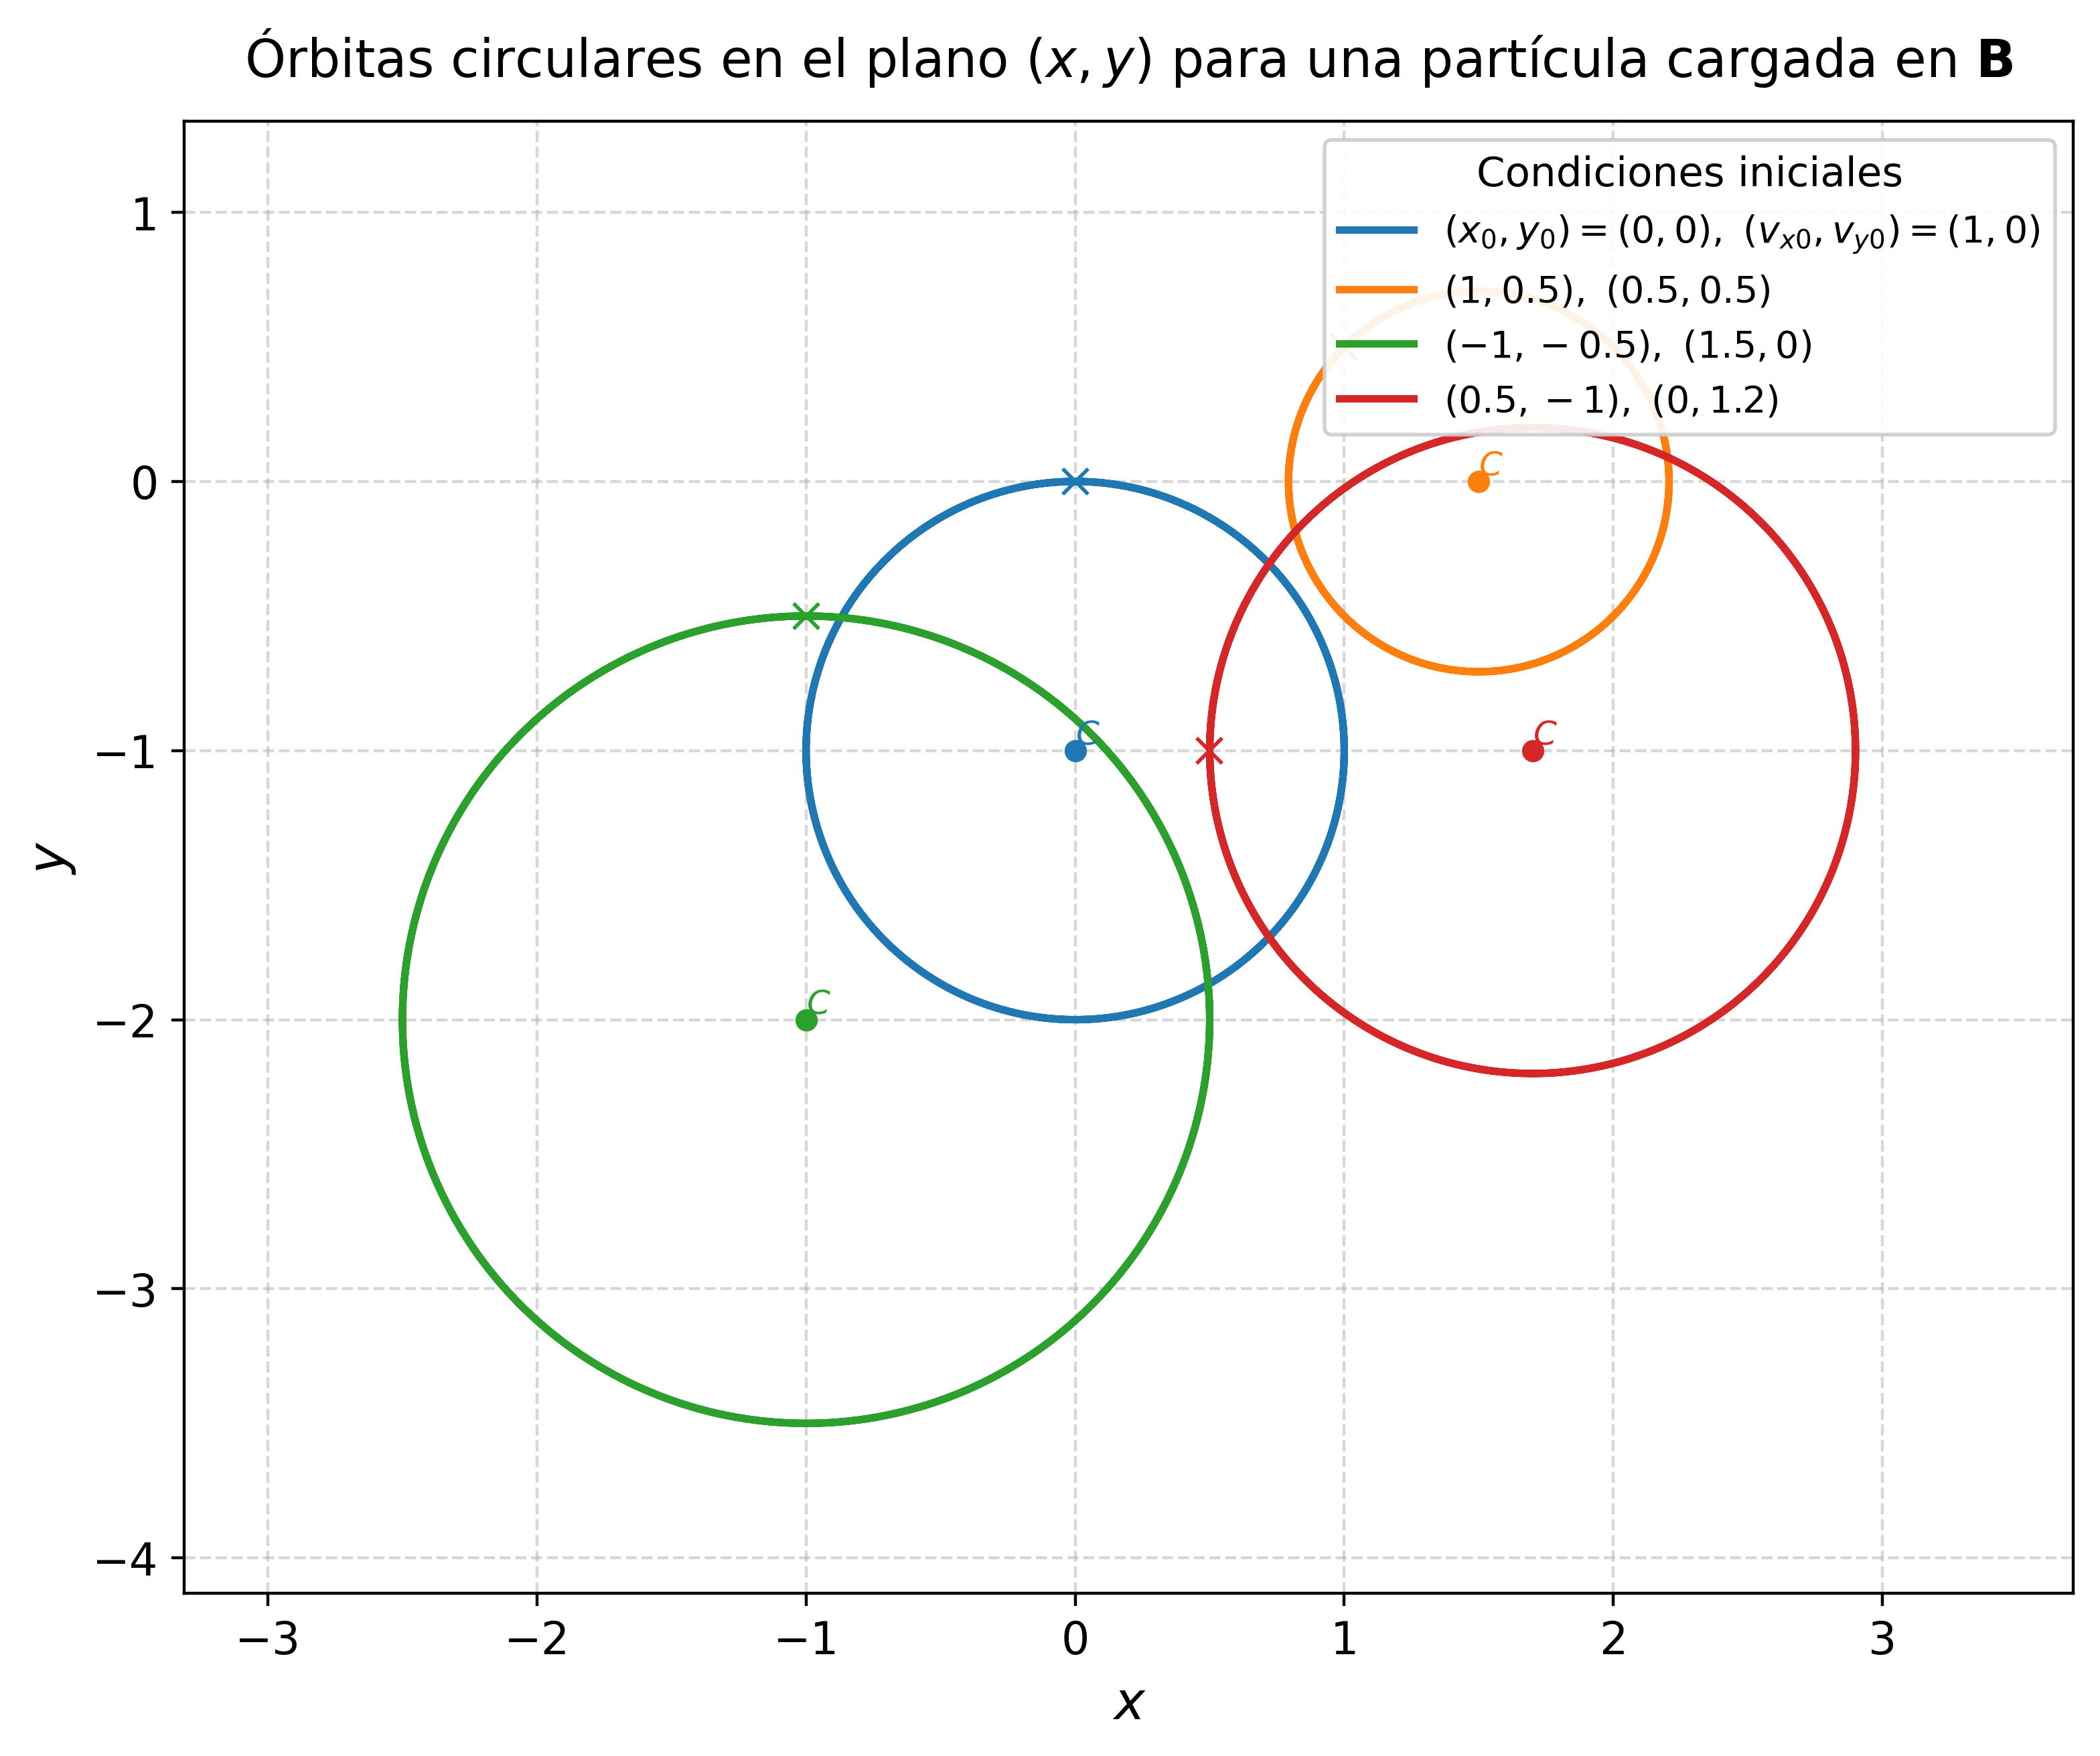
\includegraphics[width=0.7\textwidth]{orbitas_magnetico_xy.png}
  \caption{
  Órbitas circulares en el plano $(x,y)$ para una partícula cargada en un
  campo magnético uniforme $\mathbf{B}$. Cada curva corresponde a un conjunto
  distinto de condiciones iniciales $(x_{0},y_{0},v_{x0},v_{y0})$; los símbolos
  ``$\times$'' marcan la posición inicial y los puntos ``$C$'' indican los
  centros de las órbitas.
  }
  \label{fig:orbitas-magnetico-xy}
\end{figure}



%=====================================================================
%   PR 4.6 – Fuerza dependiente de \dot x y t
%=====================================================================

\begin{AGbox}[8]
\begin{enumerate}[label={{\textcolor{trueblue}{\textbf{Pr.} 4.6}}}]
  \item Una partícula de masa $m$ se mueve sobre el eje real bajo la influencia de una fuerza, tal que usando la coordenada $x$, está dada por
  \[
  \mathbf{F} = (\beta\dot{x} + \alpha t)\hat{x},
  \]
  donde $\alpha$ y $\beta$ son dos constantes reales. Determinar el potencial generalizado $U(x,\dot{x},t)$ que proporciona esta fuerza, la Lagrangiana, el Hamiltoniano y las ecuaciones de Hamilton.
\end{enumerate}
\end{AGbox}

\vspace{0.5cm}
\textcolor{Cinnabar}{\textbf{Solución:}}
\vspace{0.5cm}


La fuerza total que actúa sobre la partícula es
\begin{equation}
F(x,\dot x,t) = \beta\dot x + \alpha t.
\label{eq:fuerza}
\end{equation}

La ecuación de Newton correspondiente es
\begin{equation}
m\ddot x = \beta\dot x + \alpha t,
\label{eq:newton}
\end{equation}
que contiene dos términos claramente no conservativos:
\begin{itemize}
  \item[$\bullet$] uno proporcional a $\dot x$ (fricción o fuerza viscosa),
  \item[$\bullet$] uno proporcional al tiempo $t$ (fuerza externa explícitamente dependiente del tiempo).
\end{itemize}

Debido a esta estructura, no existe un potencial usual $U(x)$, pero sí puede existir un  
\textbf{potencial generalizado} $U(x,\dot x,t)$ que satisfaga la identidad lagrangiana
\begin{equation}
F
= \frac{d}{dt}\left(\frac{\partial U}{\partial \dot x}\right)
  - \frac{\partial U}{\partial x}.
\label{eq:fuerza-potgen}
\end{equation}

Nuestro primer objetivo será hallar tal función $U(x,\dot x,t)$.



Queremos que la ecuación \eqref{eq:fuerza-potgen} reproduzca la fuerza dada en \eqref{eq:fuerza}.  
Proponemos una forma suficientemente general:
\begin{equation}
U(x,\dot x,t) = A(t)\,\dot x^{2} + B(t)\,x.
\label{eq:U-general}
\end{equation}

\paragraph{(i) Término proporcional a $x$}

De \eqref{eq:fuerza-potgen},
\[
-\,\frac{\partial U}{\partial x} = -B(t) = \alpha t,
\]
por lo que
\begin{equation}
B(t) = -\alpha t.
\label{eq:B}
\end{equation}

\paragraph{(ii) Término proporcional a $\dot x$}

La otra parte de la fuerza debe provenir de
\[
\frac{d}{dt}\left(\frac{\partial U}{\partial\dot x}\right)
= \frac{d}{dt}\bigl( 2A(t)\dot x \bigr)
= 2A(t)\ddot x + 2\dot A(t)\dot x.
\]

Como la fuerza \eqref{eq:fuerza} **no contiene términos con $\ddot x$**, exigimos
\[
A(t)=0,
\]
para eliminar ese término por completo.

De esta forma,
\[
\frac{d}{dt}\left(\frac{\partial U}{\partial\dot x}\right)
= 0.
\]

La fuerza original contiene $\beta\dot x$, y este término debe provenir de la Lagrangiana y no del potencial generalizado.  
Por tanto el potencial correcto es simplemente

\begin{equation}
U(x,t) = -\alpha t\,x.
\label{eq:U-final}
\end{equation}

Este potencial es dependiente del tiempo, como exige el término $\alpha t$ en la fuerza.


Para reproducir el término $\beta\dot x$ de la fuerza, basta con incluir un  
coeficiente dependiente del tiempo en el término cinético.  
Planteamos entonces la Lagrangiana general

\begin{equation}
L(x,\dot x,t)
=
\frac{1}{2}M(t)\,\dot x^{2} + \alpha t\,x,
\label{eq:L-general}
\end{equation}
donde $M(t)$ es una función a determinar.

Calculamos las derivadas de Euler–Lagrange:
\[
\frac{\partial L}{\partial x} = \alpha t,
\qquad
\frac{\partial L}{\partial\dot x} = M(t)\dot x,
\]
y por lo tanto
\[
\frac{d}{dt}\left( M(t)\dot x \right)
= \dot M(t)\,\dot x + M(t)\ddot x.
\]

La ecuación de Euler–Lagrange queda entonces

\begin{equation}
\dot M(t)\,\dot x + M(t)\ddot x - \alpha t =0.
\label{eq:ELM}
\end{equation}

Queremos compararla con la ecuación real \eqref{eq:newton}:

\[
m\ddot x = \beta\dot x + \alpha t.
\]

Para igualarlas término a término es necesario imponer

\[
M(t) = m - \beta t.
\]

Sustituyendo esto en \eqref{eq:L-general}, obtenemos la Lagrangiana definitiva:

\begin{equation}
L(x,\dot x,t)
=
\frac{1}{2}(m-\beta t)\,\dot x^{2}
+ \alpha t\,x.
\label{eq:L-final}
\end{equation}

Esta Lagrangiana reproduce exactamente la ecuación de movimiento original \eqref{eq:newton}.



El momento generalizado es

\begin{equation}
p
= \frac{\partial L}{\partial\dot x}
= (m - \beta t)\,\dot x.
\label{eq:p}
\end{equation}

Despejamos la velocidad:
\begin{equation}
\dot x = 
\frac{p}{\,m-\beta t\,}.
\label{eq:xdot}
\end{equation}

El Hamiltoniano se obtiene mediante
\[
H = p\dot x - L.
\]

Usando \eqref{eq:xdot} y \eqref{eq:L-final}:

\begin{equation}
H(x,p,t)
=
\frac{p^{2}}{2(m-\beta t)}
- \alpha t\,x.
\label{eq:H-final}
\end{equation}

Este Hamiltoniano depende explícitamente del tiempo, por lo que no representa una
constante de movimiento.


Aplicamos las ecuaciones canónicas:

\[
\dot x = \frac{\partial H}{\partial p},
\qquad
\dot p = -\frac{\partial H}{\partial x}.
\]

\paragraph{Primera ecuación:}
\begin{equation}
\dot x
= \frac{p}{m-\beta t}.
\label{eq:ham-x}
\end{equation}

\paragraph{Segunda ecuación:}
\begin{equation}
\dot p
= \alpha t.
\label{eq:ham-p}
\end{equation}

\paragraph{Consistencia con la ecuación original}

Derivamos \eqref{eq:ham-x} y usamos \eqref{eq:ham-p}:

\[
\ddot x
= \frac{d}{dt}
\left(
\frac{p}{m-\beta t}
\right)
=
\frac{\alpha t}{m-\beta t}
+ \frac{p\,\beta}{(m-\beta t)^{2}}.
\]

Sustituyendo $p=(m-\beta t)\dot x$ obtenemos:

\[
\ddot x
=
\frac{\alpha t}{m-\beta t}
+ \frac{\beta}{m-\beta t}\dot x.
\]

Multiplicando por $(m-\beta t)$:

\[
m\ddot x
= \beta\dot x + \alpha t,
\]

que es precisamente la ecuación de Newton \eqref{eq:newton}.  
Esto confirma la plena consistencia de la Lagrangiana \eqref{eq:L-final} y del Hamiltoniano \eqref{eq:H-final}.

\vspace{0.4cm}
\textbf{En resumen}, para la fuerza 
\[
F = \beta\dot x + \alpha t,
\]
hemos obtenido:

\[
U(x,t) = -\alpha t\,x,
\]

\[
L = \frac{1}{2}(m-\beta t)\dot x^{2}
+ \alpha t\,x,
\]

\[
H = \frac{p^{2}}{2(m-\beta t)} - \alpha t\,x,
\]

y las ecuaciones de Hamilton \eqref{eq:ham-x}–\eqref{eq:ham-p}, que reproducen de forma exacta la dinámica dada por \eqref{eq:newton}.




%=============================
% PR. 4.7
%=============================

\begin{AGbox}[8]
\begin{enumerate}[label={{\textcolor{trueblue}{\textbf{Pr.} 4.7}}}]
  \item Para el problema de Kepler determinar: el Hamiltoniano, las ecuaciones de Hamilton, las trayectorias y constantes de movimiento.
\end{enumerate}
\end{AGbox}
\vspace{0.5cm}

\textcolor{Cinnabar}{\textbf{Solución:}} \vspace{0.5cm}

\begin{figure}[H]
\centering
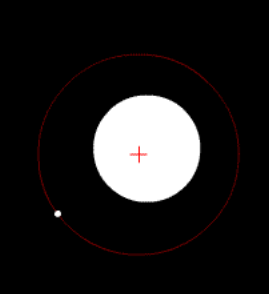
\includegraphics[width=0.42\textwidth]{problema_de_kepler.png}
\caption{\textbf{Órbita elíptica del problema de Kepler.} 
Una partícula de masa $m$ se mueve bajo el potencial central 
$U(r)=-k/r$, generando trayectorias cónicas (elipses, parábolas o 
hipérbolas). La figura ilustra el caso ligado: una órbita elíptica 
alrededor del centro atractor, característica del potencial 
inversamente proporcional a la distancia.}
\label{fig:kepler}
\end{figure}

Antes de proceder al formalismo Hamiltoniano, es útil visualizar la 
estructura geométrica del movimiento. La Figura~\ref{fig:kepler} muestra 
la trayectoria típica de una partícula sometida a un potencial de la forma 
$U(r)=-k/r$: una órbita cerrada cuando la energía total es negativa. 
Nuestro objetivo será derivar estas curvas de nivel —y sus constantes de 
movimiento asociadas— directamente desde el Hamiltoniano del sistema.

\vspace{0.4cm}
\textbf{Potencial y planteamiento del problema}

En el problema de Kepler una partícula de masa $m$ se mueve bajo un 
potencial central newtoniano
\[
U(r) = -\,\frac{k}{r},
\]
donde $k>0$ es una constante que recoge la naturaleza de la interacción. 
Por ejemplo:
\begin{itemize}
  \item[$\bullet$] En el contexto gravitatorio de dos masas puntuales $m_{1}$ y $m_{2}$,
        se tiene
        \[
          k = G\,m_{1}m_{2},
        \]
        de modo que
        \(
          U(r) = -\,\dfrac{G m_{1} m_{2}}{r}
        \).
  \item[$\bullet$] En el análogo coulombiano para dos cargas $q_{1}$ y $q_{2}$,
        \[
          k = \frac{1}{4\pi\varepsilon_{0}}\,q_{1}q_{2},
        \]
        y el potencial toma la forma
        \(
          U(r) = -\,\dfrac{1}{4\pi\varepsilon_{0}}
                 \dfrac{q_{1}q_{2}}{r}
        \)
        (atractivo si $q_{1}q_{2}<0$).
\end{itemize}

En lo que sigue, trabajaremos con la notación compacta $U(r)=-k/r$, 
entendiendo que $k$ representa el acoplamiento efectivo de la 
interacción central considerada.


Como el potencial depende únicamente del radio, resulta natural trabajar 
en coordenadas esféricas $(r,\theta,\phi)$. La energía cinética en estas 
coordenadas es
\[
T = \frac{m}{2}\Bigl(
      \dot r^{2}
      + r^{2}\dot\theta^{2}
      + r^{2}\sin^{2}\theta\,\dot\phi^{2}
    \Bigr).
\]

La Lagrangiana toma la forma usual $L = T - U$, de modo que
\begin{equation}
L(r,\theta,\phi,\dot r,\dot\theta,\dot\phi)
=
\frac{m}{2}\Bigl(
      \dot r^{2}
      + r^{2}\dot\theta^{2}
      + r^{2}\sin^{2}\theta\,\dot\phi^{2}
    \Bigr)
+ \frac{k}{r},
\label{eq:L-Kepler}
\end{equation}


%------------------------------------------------
\textcolor{trueblue}{\textbf{Momentos canónicos y Hamiltoniano}}
%------------------------------------------------

Los momentos conjugados se definen como $p_{q} = \partial L/\partial\dot q$ para
cada coordenada generalizada $q\in\{r,\theta,\phi\}$:
\begin{equation}
\begin{split}
p_{r} &= \frac{\partial L}{\partial \dot r}
      = m\dot r
      \qquad\Rightarrow\qquad
      \dot r = \frac{p_{r}}{m} \\[4pt]
p_{\theta} &= \frac{\partial L}{\partial \dot\theta}
           = m r^{2}\dot\theta
           \qquad\Rightarrow\qquad
           \dot\theta = \frac{p_{\theta}}{m r^{2}} \\[4pt]
p_{\phi} &= \frac{\partial L}{\partial \dot\phi}
          = m r^{2}\sin^{2}\theta\,\dot\phi
          \qquad\Rightarrow\qquad
          \dot\phi = \frac{p_{\phi}}{m r^{2}\sin^{2}\theta}
\end{split}
\label{eq:momentos-Kepler}
\end{equation}

El Hamiltoniano se obtiene mediante la transformación de Legendre
\[
H = \sum_{q}\,p_{q}\dot q - L
\]
expresándolo en términos de $(r,\theta,\phi,p_{r},p_{\theta},p_{\phi})$ usando
\eqref{eq:momentos-Kepler}. El resultado es
\begin{equation}
H(r,\theta,\phi,p_{r},p_{\theta},p_{\phi})
=
\frac{1}{2m}\left(
p_{r}^{2}
+ \frac{p_{\theta}^{2}}{r^{2}}
+ \frac{p_{\phi}^{2}}{r^{2}\sin^{2}\theta}
\right)
- \frac{k}{r}
\label{eq:H-Kepler}
\end{equation}

Como $H$ no depende explícitamente del tiempo, representa la \textbf{energía
total} del sistema.

%------------------------------------------------
\textcolor{trueblue}{\textbf{Ecuaciones de Hamilton}}
%------------------------------------------------

Las ecuaciones canónicas son
\[
\dot q_{i} = \frac{\partial H}{\partial p_{i}},
\qquad
\dot p_{i} = -\,\frac{\partial H}{\partial q_{i}}
\]

Aplicándolas al Hamiltoniano \eqref{eq:H-Kepler} obtenemos:

\medskip
\textbf{Para la coordenada radial $r$:}
\begin{equation}
\begin{split}
\dot r &= \frac{\partial H}{\partial p_{r}}
       = \frac{p_{r}}{m} \\[4pt]
\dot p_{r} &= -\,\frac{\partial H}{\partial r}
          = \frac{p_{\theta}^{2}}{m r^{3}}
            + \frac{p_{\phi}^{2}}{m r^{3}\sin^{2}\theta}
            - \frac{k}{r^{2}}
\end{split}
\label{eq:Ham-r}
\end{equation}

\textbf{Para la coordenada polar $\theta$:}
\begin{equation}
\begin{split}
\dot\theta &= \frac{\partial H}{\partial p_{\theta}}
           = \frac{p_{\theta}}{m r^{2}} \\[4pt]
\dot p_{\theta} &= -\,\frac{\partial H}{\partial\theta}
               = \frac{p_{\phi}^{2}\cos\theta}{m r^{2}\sin^{3}\theta}
\end{split}
\label{eq:Ham-theta}
\end{equation}

\textbf{Para la coordenada azimutal $\phi$:}
\begin{equation}
\begin{split}
\dot\phi &= \frac{\partial H}{\partial p_{\phi}}
        = \frac{p_{\phi}}{m r^{2}\sin^{2}\theta} \\[4pt]
\dot p_{\phi} &= -\,\frac{\partial H}{\partial\phi}
             = 0
\end{split}
\label{eq:Ham-phi}
\end{equation}

La última ecuación muestra que $p_{\phi}$ es una \textbf{constante de
movimiento}.

%------------------------------------------------
\textcolor{trueblue}{\textbf{Constantes de movimiento}}
%------------------------------------------------

Del Hamiltoniano \eqref{eq:H-Kepler} y de las ecuaciones
\eqref{eq:Ham-r}–\eqref{eq:Ham-phi} se identifican varias cantidades
conservadas:

\begin{itemize}
  \item[$\bullet$] \textbf{Energía total}  
  Como $\partial H/\partial t = 0$, el Hamiltoniano se conserva
  \begin{equation}
  H = E = \text{constante}
  \label{eq:E-constante}
  \end{equation}

  \item[$\bullet$] \textbf{Componente $z$ del momento angular}  
  De \eqref{eq:Ham-phi} se sigue que
  \begin{equation}
  \dot p_{\phi} = 0
  \qquad\Rightarrow\qquad
  p_{\phi} = \text{constante}
  \label{eq:Lz-constante}
  \end{equation}
  lo cual refleja que $\phi$ es una coordenada cíclica

  \item[$\bullet$] \textbf{Módulo cuadrado del momento angular}  
  En el problema de fuerzas centrales, el vector momento angular
  $\vec L = \vec r \times \vec p$ se conserva. En coordenadas esféricas su
  módulo verifica
  \begin{equation}
  L^{2} = p_{\theta}^{2}
       + \frac{p_{\phi}^{2}}{\sin^{2}\theta}
  \label{eq:L2}
  \end{equation}
  y se puede mostrar que $\dot L^{2} = 0$, de modo que $L^{2}$ es constante
\end{itemize}

Más allá de estas cantidades, el problema de Kepler posee una simetría adicional
codificada en el \textbf{vector de Laplace–Runge–Lenz}, también conservado,
que está relacionado con la forma cónica de las órbitas. Aquí no lo derivamos,
pero es la constante de movimiento responsable de que todas las órbitas
ligadas sean elipses cerradas.

%------------------------------------------------
\textcolor{trueblue}{\textbf{Comentario sobre el problema de dos cuerpos y la masa reducida}}
%------------------------------------------------

El planteamiento anterior puede interpretarse de manera más general como la
descripción del \emph{problema de dos cuerpos} reducido a un problema
equivalente de una sola partícula. Consideremos dos masas puntuales
$m_{1}$ y $m_{2}$ en las posiciones $\vec r_{1}$ y $\vec r_{2}$, que se
atraen mediante el potencial newtoniano
\[
U(\vec r_{1},\vec r_{2})
= -\,\frac{G m_{1} m_{2}}{\lvert \vec r_{1} - \vec r_{2}\rvert}
= -\,\frac{k}{r},
\qquad
r = \lvert\vec r_{1}-\vec r_{2}\rvert
\]

La energía cinética total es
\[
T = \frac{1}{2}m_{1}\dot{\vec r}_{1}^{\,2}
  + \frac{1}{2}m_{2}\dot{\vec r}_{2}^{\,2}
\]

Es conveniente introducir las coordenadas de \textbf{centro de masa} y
\textbf{relativas}:
\begin{equation}
\vec R = \frac{m_{1}\vec r_{1} + m_{2}\vec r_{2}}{m_{1}+m_{2}},
\qquad
\vec r = \vec r_{1} - \vec r_{2}
\label{eq:CM-rel}
\end{equation}
junto con la masa total $M = m_{1}+m_{2}$ y la \textbf{masa reducida}
\begin{equation}
\mu = \frac{m_{1}m_{2}}{m_{1}+m_{2}}
\label{eq:masa-reducida}
\end{equation}

En estas variables, el cinético se separa como
\[
T = \frac{1}{2}M\dot{\vec R}^{\,2}
  + \frac{1}{2}\mu\,\dot{\vec r}^{\,2}
\]
y el potencial sólo depende de $\vec r$, de modo que la Lagrangiana total
se escribe
\[
L(\vec R,\dot{\vec R},\vec r,\dot{\vec r})
= \underbrace{\frac{1}{2}M\dot{\vec R}^{\,2}}_{L_{\text{CM}}}
+ \underbrace{\left[
    \frac{1}{2}\mu\,\dot{\vec r}^{\,2}
    + \frac{k}{r}
  \right]}_{L_{\text{rel}}}
\]

La dinámica se separa entonces en:

\begin{itemize}
  \item[$\bullet$] un movimiento de \textbf{centro de masa} descrito por
        $L_{\text{CM}} = \tfrac{1}{2}M\dot{\vec R}^{\,2}$, que corresponde a
        una partícula libre de masa $M$

   \item[$\bullet$] un movimiento \textbf{relativo} gobernado por
        \[
        L_{\text{rel}} = \frac{1}{2}\mu\,\dot{\vec r}^{\,2} + \frac{k}{r}
        \]
        que tiene exactamente la forma de \eqref{eq:L-Kepler} si se identifica
        $m \equiv \mu$
\end{itemize}

El Hamiltoniano relativo asociado es
\[
H_{\text{rel}}(\vec r,\vec p)
= \frac{\vec p^{\,2}}{2\mu} - \frac{k}{r}
\]
y coincide con \eqref{eq:H-Kepler} al reemplazar $m$ por la masa reducida
$\mu$. En el límite en que una de las masas es mucho mayor que la otra
(por ejemplo, el Sol y un planeta), se tiene $\mu \approx m_{\text{planeta}}$,
y es habitual escribir simplemente $m$ como hemos hecho arriba. Esta
interpretación aclara que el problema de Kepler es, en realidad, la
descripción del movimiento relativo de dos cuerpos bajo interacción central.

%------------------------------------------------
\textcolor{trueblue}{\textbf{Reducción al plano y ecuación de las trayectorias}}
%------------------------------------------------

Como $\vec L$ es constante y distinto de cero, el movimiento queda restringido
a un plano perpendicular a $\vec L$. Podemos elegir el sistema de referencia de
modo que este plano coincida con el plano ecuatorial:
\[
\theta = \frac{\pi}{2}
\]

En estas condiciones
\[
\sin\theta = 1,
\qquad
\cos\theta = 0,
\qquad
p_{\theta} = 0
\]
y la única componente no nula del momento angular es
\[
l \equiv p_{\phi} = \text{constante}
\]

El Hamiltoniano \eqref{eq:H-Kepler} se reduce entonces a
\begin{equation}
H = \frac{1}{2m}\left(p_{r}^{2} + \frac{l^{2}}{r^{2}}\right) - \frac{k}{r}
= E
\label{eq:H-reducido}
\end{equation}

De \eqref{eq:H-reducido} se despeja el momento radial
\begin{equation}
p_{r}
= \pm\sqrt{\,2m\left(E + \frac{k}{r}\right)
          - \frac{l^{2}}{r^{2}}\,}
\label{eq:pr-energia}
\end{equation}

Por otro lado, del hecho de que $p_{r} = m\dot r$ y
\[
\dot\phi = \frac{l}{m r^{2}}
\]
obtenemos, usando la regla de la cadena,
\begin{equation}
p_{r} = m\frac{dr}{dt}
= m\frac{dr}{d\phi}\frac{d\phi}{dt}
= \frac{l}{r^{2}}\frac{dr}{d\phi}
\label{eq:pr-dr-dphi}
\end{equation}

Igualando \eqref{eq:pr-energia} y \eqref{eq:pr-dr-dphi} se tiene
\begin{equation}
\frac{l}{r^{2}}\frac{dr}{d\phi}
=
\pm\sqrt{\,2mE + \frac{2mk}{r} - \frac{l^{2}}{r^{2}}\,}
\label{eq:edo-r-phi}
\end{equation}

Para integrar esta ecuación es conveniente introducir la variable
\begin{equation}
u(\phi) \equiv \frac{1}{r(\phi)}
\label{eq:def-u}
\end{equation}
con lo cual $dr/d\phi = -u^{-2}du/d\phi$. Sustituyendo en
\eqref{eq:edo-r-phi} y reordenando se llega a la ecuación diferencial estándar
para el problema de Kepler, cuya integración conduce a
\begin{equation}
u(\phi)
= \frac{mk}{l^{2}}\Bigl[1 + e\cos\bigl(\phi-\phi_{0}\bigr)\Bigr]
\label{eq:u-orbita}
\end{equation}
o, en términos de $r$,
\begin{equation}
\frac{1}{r(\phi)}
= \frac{mk}{l^{2}}\Bigl[1 + e\cos\bigl(\phi-\phi_{0}\bigr)\Bigr]
\label{eq:orbita-conica}
\end{equation}
donde $\phi_{0}$ es una constante de integración que fija la orientación de la
órbita, y
\begin{equation}
e
=
\sqrt{1 + \frac{2 E l^{2}}{m k^{2}}}
\label{eq:excentricidad}
\end{equation}
es la \textbf{excentricidad} de la trayectoria.

\medskip
\noindent
La ecuación \eqref{eq:orbita-conica} muestra que las trayectorias del problema
de Kepler son secciones cónicas (elipses, parábolas o hipérbolas) en el plano
$(r,\phi)$, determinadas por los valores de la energía $E$ y del momento
angular $l$. En particular:

\begin{itemize}
  \item[$\bullet$] $0 \le e < 1$  $\Rightarrow$ órbitas elípticas (estado ligado)
  \item[$\bullet$] $e = 1$        $\Rightarrow$ órbita parabólica (energía de escape)
  \item[$\bullet$] $e > 1$        $\Rightarrow$ órbita hiperbólica (trayectoria de dispersión)
\end{itemize}

Así, el formalismo Hamiltoniano reproduce de manera elegante la estructura
geométrica del problema de Kepler y hace explícitas sus constantes de
movimiento fundamentales: $E$, $\vec L$.



\begin{AGbox}[8]
\begin{enumerate}[label={{\textcolor{trueblue}{\textbf{Pr.} 4.8}}}]
  \item Dos partículas puntuales de masa $m$ están unidas por una barra rígida de masa despreciable de longitud $l$, cuyo centro está obligado a moverse en un círculo de radio $a$ sobre el plano $x = 0$. El sistema se mueve bajo la acción del campo gravitacional de la tierra dado por $\mathbf{g} = -g\hat{z}$. Obtener: la Lagrangiana, el Hamiltoniano y las ecuaciones de Hamilton.
\end{enumerate}
\end{AGbox}
\vspace{0.5cm}

\textcolor{Cinnabar}{\textbf{Solución:}} \vspace{0.5cm}

\begin{figure}[H]
  \centering
  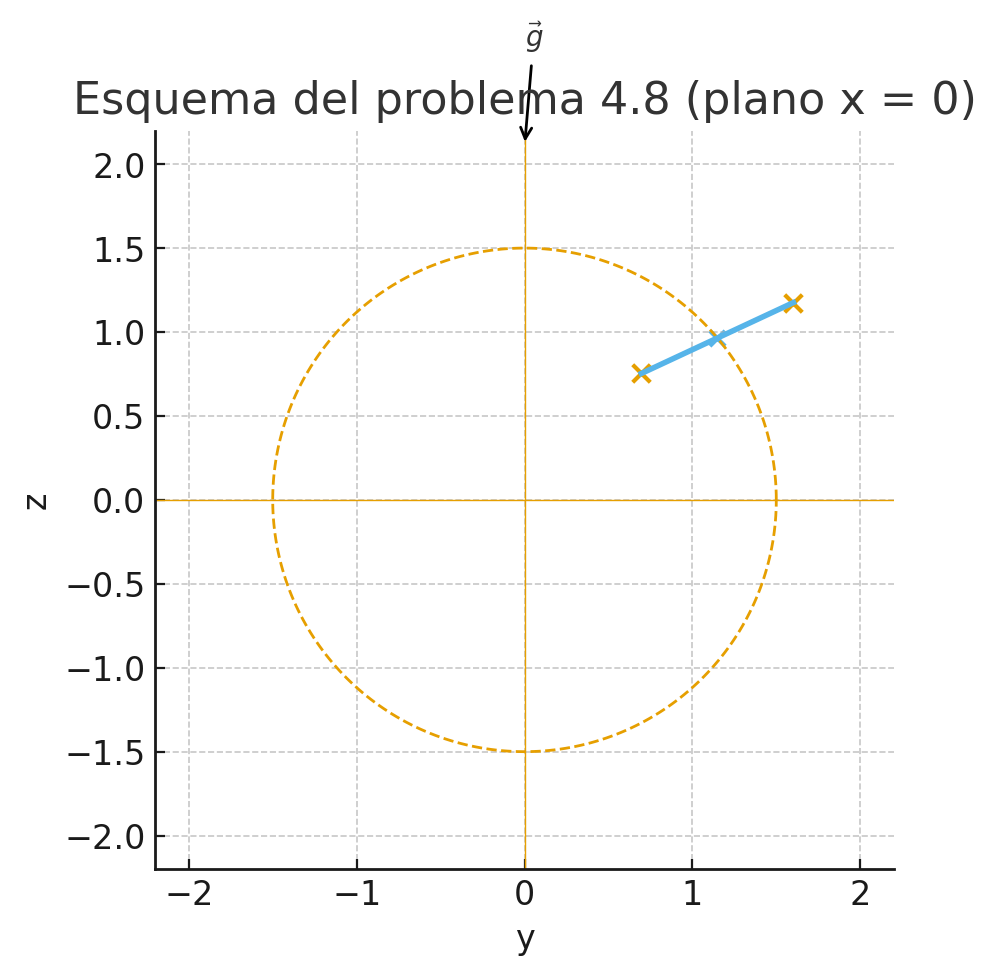
\includegraphics[width=0.45\textwidth]{xd.png}
  \caption{Esquema del problema 4.8. El centro de la barra de longitud $l$
  describe un círculo de radio $a$ en el plano $x=0$, mientras las masas $m$
  se encuentran en los extremos y el campo gravitacional apunta en dirección
  $-\,\hat z$.}
  \label{fig:barra-circulo}
\end{figure}



El sistema está contenido en el plano $x=0$, por lo que basta trabajar en el
plano $yz$. Dos partículas puntuales de masa $m$ están unidas por una barra
rígida de longitud $l$ y masa despreciable. El \textbf{centro de la barra} se
mueve sobre una circunferencia de radio $a$ en el plano $x=0$, bajo la acción
del campo gravitacional uniforme
\[
\vec g = -\,g\,\hat z
\]

Elegimos como coordenadas generalizadas
\begin{itemize}
  \item[$\bullet$] $\theta$: ángulo que forma el vector desde el origen hasta el centro
  de la barra con la \textbf{vertical negativa} $-\hat z$ en el plano $yz$
  \item[$\bullet$] $\phi$: ángulo que forma la barra con la \textbf{vertical} en el
  mismo plano $yz$
\end{itemize}

Con esta convención, las coordenadas del centro de la barra $(y_{\text{cm}},
z_{\text{cm}})$ son
\begin{equation}
\begin{split}
y_{\text{cm}} &= a\sin\theta \\[4pt]
z_{\text{cm}} &= -\,a\cos\theta
\end{split}
\label{eq:cm-48}
\end{equation}

Las masas están situadas a una distancia $l/2$ del centro, en direcciones
opuestas a lo largo de la barra.

\medskip
\textbf{Masa 1} (situada “hacia abajo” cuando $\phi=0$):
\begin{equation}
\begin{split}
y_{1} &= y_{\text{cm}} + \frac{l}{2}\,\sin\phi
      = a\sin\theta + \frac{l}{2}\,\sin\phi \\[4pt]
z_{1} &= z_{\text{cm}} - \frac{l}{2}\,\cos\phi
      = -\,a\cos\theta - \frac{l}{2}\,\cos\phi
\end{split}
\label{eq:pos-masa1}
\end{equation}

\textbf{Masa 2} (situada en la dirección opuesta):
\begin{equation}
\begin{split}
y_{2} &= y_{\text{cm}} - \frac{l}{2}\,\sin\phi
      = a\sin\theta - \frac{l}{2}\,\sin\phi \\[4pt]
z_{2} &= z_{\text{cm}} + \frac{l}{2}\,\cos\phi
      = -\,a\cos\theta + \frac{l}{2}\,\cos\phi
\end{split}
\label{eq:pos-masa2}
\end{equation}

%------------------------------------------------
\textcolor{trueblue}{\textbf{Energía cinética $T$}}
%------------------------------------------------

La energía cinética total es la suma de las contribuciones de cada masa
\begin{equation}
T = \frac{1}{2}m v_{1}^{2} + \frac{1}{2}m v_{2}^{2}
\label{eq:T-def-48}
\end{equation}
donde $v_{i}^{2} = \dot y_{i}^{2} + \dot z_{i}^{2}$ para $i=1,2$

\medskip
\textbf{Velocidades de la masa 1.} Derivamos \eqref{eq:pos-masa1} respecto al
tiempo
\begin{equation}
\begin{split}
\dot y_{1} &= a\dot\theta\cos\theta
           + \frac{l}{2}\dot\phi\cos\phi \\[4pt]
\dot z_{1} &= a\dot\theta\sin\theta
           + \frac{l}{2}\dot\phi\sin\phi
\end{split}
\label{eq:vel-masa1}
\end{equation}

Entonces
\begin{equation}
\begin{split}
v_{1}^{2}
&= \dot y_{1}^{2} + \dot z_{1}^{2} \\[4pt]
&=
\bigl(a\dot\theta\cos\theta + \tfrac{l}{2}\dot\phi\cos\phi\bigr)^{2}
+
\bigl(a\dot\theta\sin\theta + \tfrac{l}{2}\dot\phi\sin\phi\bigr)^{2}
\end{split}
\label{eq:v1-cuadrada-raw}
\end{equation}

Desarrollando los cuadrados y agrupando términos aparece de forma natural la
combinación
\[
\cos^{2}\theta + \sin^{2}\theta = 1,
\qquad
\cos^{2}\phi + \sin^{2}\phi = 1,
\]
así como el coseno de la diferencia
\[
\cos(\theta-\phi)
= \cos\theta\cos\phi + \sin\theta\sin\phi
\]

Con estas identidades, \eqref{eq:v1-cuadrada-raw} se simplifica a
\begin{equation}
v_{1}^{2}
= a^{2}\dot\theta^{2}
+ \frac{l^{2}}{4}\dot\phi^{2}
+ a l\,\dot\theta\dot\phi\cos(\theta-\phi)
\label{eq:v1-cuadrada}
\end{equation}

\medskip
\textbf{Velocidades de la masa 2.} Derivando \eqref{eq:pos-masa2} se obtiene
\begin{equation}
\begin{split}
\dot y_{2} &= a\dot\theta\cos\theta
           - \frac{l}{2}\dot\phi\cos\phi \\[4pt]
\dot z_{2} &= a\dot\theta\sin\theta
           - \frac{l}{2}\dot\phi\sin\phi
\end{split}
\label{eq:vel-masa2}
\end{equation}

Un cálculo análogo al anterior da
\begin{equation}
v_{2}^{2}
= a^{2}\dot\theta^{2}
+ \frac{l^{2}}{4}\dot\phi^{2}
- a l\,\dot\theta\dot\phi\cos(\theta-\phi)
\label{eq:v2-cuadrada}
\end{equation}

\medskip
\textbf{Energía cinética total.} Sumando \eqref{eq:v1-cuadrada} y
\eqref{eq:v2-cuadrada} se observa que los términos cruzados se cancelan
\begin{equation}
\begin{split}
v_{1}^{2} + v_{2}^{2}
&= \Bigl[a^{2}\dot\theta^{2}
+ \tfrac{l^{2}}{4}\dot\phi^{2}
+ a l\,\dot\theta\dot\phi\cos(\theta-\phi)\Bigr]
 \\[2pt]
&\quad
+ \Bigl[a^{2}\dot\theta^{2}
+ \tfrac{l^{2}}{4}\dot\phi^{2}
- a l\,\dot\theta\dot\phi\cos(\theta-\phi)\Bigr] \\[4pt]
&= 2a^{2}\dot\theta^{2} + \frac{l^{2}}{2}\dot\phi^{2}
\end{split}
\label{eq:v1-mas-v2}
\end{equation}

Sustituyendo \eqref{eq:v1-mas-v2} en \eqref{eq:T-def-48} se obtiene
\begin{equation}
\begin{split}
T
&= \frac{1}{2}m\bigl(v_{1}^{2} + v_{2}^{2}\bigr) \\[4pt]
&= \frac{1}{2}m\left(2a^{2}\dot\theta^{2}
                  + \frac{l^{2}}{2}\dot\phi^{2}\right)
\end{split}
\label{eq:T-48-mid}
\end{equation}
es decir
\begin{equation}
T
= m a^{2}\dot\theta^{2}
+ \frac{1}{4}m l^{2}\dot\phi^{2}
\label{eq:T-48}
\end{equation}

%------------------------------------------------
\textcolor{trueblue}{\textbf{Energía potencial gravitatoria $U$}}
%------------------------------------------------

En el campo gravitacional uniforme $\vec g = -g\,\hat z$, la energía potencial
de cada masa es $U_{i} = m g z_{i}$. Por lo tanto
\begin{equation}
U = m g z_{1} + m g z_{2}
= m g\bigl(z_{1} + z_{2}\bigr)
\label{eq:U-def-48}
\end{equation}

A partir de \eqref{eq:pos-masa1}–\eqref{eq:pos-masa2}, la suma de alturas es
\begin{equation}
\begin{split}
z_{1} + z_{2}
&= \bigl(-a\cos\theta - \tfrac{l}{2}\cos\phi\bigr)
 + \bigl(-a\cos\theta + \tfrac{l}{2}\cos\phi\bigr) \\[4pt]
&= -2a\cos\theta
\end{split}
\label{eq:z1-mas-z2}
\end{equation}

Sustituyendo \eqref{eq:z1-mas-z2} en \eqref{eq:U-def-48} se obtiene
\begin{equation}
U
= -\,2 m g a\cos\theta
\label{eq:U-48}
\end{equation}
es decir, la energía potencial depende únicamente del ángulo $\theta$ que fija
la altura del centro de la barra

%------------------------------------------------
\textcolor{trueblue}{\textbf{Lagrangiana del sistema}}
%------------------------------------------------

La Lagrangiana se define como
\[
L = T - U
\]
Sustituyendo \eqref{eq:T-48} y \eqref{eq:U-48} se obtiene
\begin{equation}
L(\theta,\phi,\dot\theta,\dot\phi)
= m a^{2}\dot\theta^{2}
+ \frac{1}{4}m l^{2}\dot\phi^{2}
+ 2 m g a\cos\theta
\label{eq:L-48}
\end{equation}

Nótese que $\phi$ no aparece explícitamente en \eqref{eq:L-48}, lo cual
anticipa la existencia de una constante de movimiento asociada a esta
coordenada cíclica

%------------------------------------------------
\textcolor{trueblue}{\textbf{Momentos canónicos y Hamiltoniano}}
%------------------------------------------------

Los momentos conjugados se definen como
\[
p_{q} = \frac{\partial L}{\partial\dot q}
\]
A partir de \eqref{eq:L-48} obtenemos
\begin{equation}
\begin{split}
p_{\theta}
&= \frac{\partial L}{\partial\dot\theta}
 = 2 m a^{2}\dot\theta
 \qquad\Rightarrow\qquad
 \dot\theta = \frac{p_{\theta}}{2 m a^{2}} \\[6pt]
p_{\phi}
&= \frac{\partial L}{\partial\dot\phi}
 = \frac{1}{2}m l^{2}\dot\phi
 \qquad\Rightarrow\qquad
 \dot\phi = \frac{2 p_{\phi}}{m l^{2}}
\end{split}
\label{eq:momentos-48}
\end{equation}

El Hamiltoniano se obtiene mediante la transformación de Legendre
\begin{equation}
H(\theta,\phi,p_{\theta},p_{\phi})
= \dot\theta\,p_{\theta} + \dot\phi\,p_{\phi} - L
\label{eq:H-Legendre-48}
\end{equation}
donde $\dot\theta$ y $\dot\phi$ deben reescribirse en términos de
$p_{\theta}$ y $p_{\phi}$ usando \eqref{eq:momentos-48}. Equivalentemente,
como el sistema es conservativo, $H$ coincide con la energía total $T+U$
expresada en variables canónicas. El resultado es
\begin{equation}
H(\theta,\phi,p_{\theta},p_{\phi})
=
\frac{p_{\theta}^{2}}{4 m a^{2}}
+ \frac{p_{\phi}^{2}}{m l^{2}}
- 2 m g a\cos\theta
\label{eq:H-48}
\end{equation}

Obsérvese que $H$ no depende explícitamente del tiempo, por lo que representa
una constante de movimiento (la energía)

%------------------------------------------------
\textcolor{trueblue}{\textbf{Ecuaciones de Hamilton y constantes de movimiento}}
%------------------------------------------------

Las ecuaciones canónicas para las coordenadas $(\theta,\phi)$ y sus momentos
conjugados $(p_{\theta},p_{\phi})$ se obtienen de
\[
\dot q = \frac{\partial H}{\partial p_{q}},
\qquad
\dot p_{q} = -\,\frac{\partial H}{\partial q}
\]

\medskip
\textbf{Para la coordenada $\theta$:}
\begin{equation}
\begin{split}
\dot\theta
&= \frac{\partial H}{\partial p_{\theta}}
 = \frac{p_{\theta}}{2 m a^{2}} \\[6pt]
\dot p_{\theta}
&= -\,\frac{\partial H}{\partial\theta}
 = -\,\frac{\partial}{\partial\theta}
    \bigl[-2 m g a\cos\theta\bigr]
 = -\,2 m g a\sin\theta
\end{split}
\label{eq:Ham-theta-48}
\end{equation}

\textbf{Para la coordenada $\phi$:}
\begin{equation}
\begin{split}
\dot\phi
&= \frac{\partial H}{\partial p_{\phi}}
 = \frac{2 p_{\phi}}{m l^{2}} \\[6pt]
\dot p_{\phi}
&= -\,\frac{\partial H}{\partial\phi}
 = 0
\end{split}
\label{eq:Ham-phi-48}
\end{equation}

La ecuación $\dot p_{\phi} = 0$ indica que $p_{\phi}$ es una
\textbf{constante de movimiento}, consecuencia de que $\phi$ es una coordenada
cíclica en la Lagrangiana \eqref{eq:L-48}. Además, como $H$ no depende del
tiempo, la energía dada por \eqref{eq:H-48} también se conserva durante toda
la evolución del sistema

\medskip
En resumen, el sistema equivalente es un movimiento acoplado en la coordenada
$\theta$ (tipo péndulo) y un movimiento de rotación uniforme alrededor de la
barra descrito por $\phi$, con $p_{\phi}$ constante y energía total $H$
constante. \vspace{0.5cm}



\begin{AGbox}[8]
\begin{enumerate}[label={{\textcolor{trueblue}{\textbf{Pr.} 4.9}}}]
  \item Hemos demostrado que el Lagrangiano
  \[
  \mathcal{L}_{H}(q,p,\dot{q},\dot{p},t)=p\dot{q}-H(q,p,t),
  \]
  proporciona las ecuaciones de Hamilton. Investigar que ecuaciones proporciona el Lagrangiano
  \[
  \mathcal{L}'_{H}\equiv \mathcal{L}_{H}+\frac{dF(q,p,t)}{dt},
  \]
  donde $F(q,p,t)$ es una función diferenciable en cada uno de sus argumentos.
\end{enumerate}
\end{AGbox}
\vspace{0.5cm}

\textcolor{Cinnabar}{\textbf{Solución:}} \vspace{0.5cm}

El problema parte del \textbf{Lagrangiano de espacio de fases}
\begin{equation}
  \mathcal{L}_{H}(q,p,\dot q,\dot p,t)
  = p\,\dot q - H(q,p,t)
\end{equation}
para el cual ya se ha demostrado que las ecuaciones de Euler--Lagrange
reproducen las ecuaciones de Hamilton.  

Ahora se introduce un nuevo Lagrangiano
\begin{equation}
  \mathcal{L}'_{H}(q,p,\dot q,\dot p,t)
  \equiv \mathcal{L}_{H}
  + \frac{dF(q,p,t)}{dt}
  \label{eq:L-prime-def}
\end{equation}
donde $F(q,p,t)$ es una función diferenciable de $q$, $p$ y $t$.  
La pregunta es: \emph{¿cambian las ecuaciones de movimiento al añadir esta derivada total}?

La idea física es que añadir una derivada total al Lagrangiano sólo modifica el
valor de la acción en los extremos de la trayectoria, pero no cambia las
ecuaciones de Euler–Lagrange. A continuación se verifica esto de manera
explícita en el formalismo de espacio de fases.

Usamos la regla de la cadena para escribir
\begin{equation}
  \frac{dF}{dt}
  = \frac{\partial F}{\partial q}\,\dot q
  + \frac{\partial F}{\partial p}\,\dot p
  + \frac{\partial F}{\partial t}
  \label{eq:dFdt}
\end{equation}

Sustituyendo \eqref{eq:dFdt} en \eqref{eq:L-prime-def} se obtiene la forma
explícita de la nueva Lagrangiana
\begin{equation}
  \mathcal{L}'_{H}
  = p\,\dot q - H(q,p,t)
    + \frac{\partial F}{\partial q}\,\dot q
    + \frac{\partial F}{\partial p}\,\dot p
    + \frac{\partial F}{\partial t}
  \label{eq:L-prime-expl}
\end{equation}

A partir de esta expresión aplicamos las ecuaciones de Euler--Lagrange para
las coordenadas generalizadas $q$ y $p$.

%------------------------------------------------
\textcolor{trueblue}{\textbf{Ecuación de Euler–Lagrange para $q$}}
%------------------------------------------------

La ecuación de Euler–Lagrange asociada a $q$ es
\begin{equation}
  \frac{d}{dt}
  \left(
    \frac{\partial \mathcal{L}'_{H}}{\partial \dot q}
  \right)
  -
  \frac{\partial \mathcal{L}'_{H}}{\partial q}
  = 0
  \label{eq:EL-q}
\end{equation}

\paragraph{Derivada parcial respecto a $\dot q$}

De \eqref{eq:L-prime-expl} se ve que los términos que dependen de $\dot q$ son
$p\,\dot q$ y $(\partial F/\partial q)\,\dot q$, por lo tanto
\begin{equation}
  \frac{\partial \mathcal{L}'_{H}}{\partial \dot q}
  = p + \frac{\partial F}{\partial q}
  \label{eq:dLprime-ddotq}
\end{equation}

\paragraph{Serivada temporal total}

Derivando \eqref{eq:dLprime-ddotq} con respecto al tiempo
\begin{equation}
\begin{split}
  \frac{d}{dt}
  \left(
    \frac{\partial \mathcal{L}'_{H}}{\partial \dot q}
  \right)
  &=
  \frac{d}{dt}
  \left(
    p + \frac{\partial F}{\partial q}
  \right)
  \\
  &=
  \dot p
  + \frac{d}{dt}\left(\frac{\partial F}{\partial q}\right)
  \\
  &=
  \dot p
  + \frac{\partial^{2}F}{\partial q^{2}}\,\dot q
  + \frac{\partial^{2}F}{\partial p\,\partial q}\,\dot p
  + \frac{\partial^{2}F}{\partial t\,\partial q}
\end{split}
\label{eq:d-dt-dLprime-ddotq}
\end{equation}

\paragraph{Derivada parcial respecto a $q$}

Ahora derivamos \eqref{eq:L-prime-expl} con respecto a $q$.  
El término $p\,\dot q$ no depende de $q$, mientras que $H$ y $F$ sí dependen
de $q$
\begin{equation}
\begin{split}
  \frac{\partial \mathcal{L}'_{H}}{\partial q}
  &=
  -\,\frac{\partial H}{\partial q}
  +
  \frac{\partial}{\partial q}
  \left(
    \frac{\partial F}{\partial q}\,\dot q
    + \frac{\partial F}{\partial p}\,\dot p
    + \frac{\partial F}{\partial t}
  \right)
  \\
  &=
  -\,\frac{\partial H}{\partial q}
  + \frac{\partial^{2}F}{\partial q^{2}}\,\dot q
  + \frac{\partial^{2}F}{\partial q\,\partial p}\,\dot p
  + \frac{\partial^{2}F}{\partial q\,\partial t}
\end{split}
\label{eq:dLprime-dq}
\end{equation}

\paragraph{Sustituimos en la ecuación de Euler–Lagrange}

Sustituyendo \eqref{eq:d-dt-dLprime-ddotq} y \eqref{eq:dLprime-dq} en
\eqref{eq:EL-q} se obtiene
\begin{equation}
\begin{split}
  &\left[
    \dot p
    + \frac{\partial^{2}F}{\partial q^{2}}\,\dot q
    + \frac{\partial^{2}F}{\partial p\,\partial q}\,\dot p
    + \frac{\partial^{2}F}{\partial t\,\partial q}
  \right]
  -
  \left[
    -\,\frac{\partial H}{\partial q}
    + \frac{\partial^{2}F}{\partial q^{2}}\,\dot q
    + \frac{\partial^{2}F}{\partial q\,\partial p}\,\dot p
    + \frac{\partial^{2}F}{\partial q\,\partial t}
  \right]
  = 0
\end{split}
\end{equation}

Los términos con segundas derivadas de $F$ son idénticos en ambos corchetes
y se cancelan gracias a la conmutatividad de las derivadas parciales mixtas
\[
\frac{\partial^{2}F}{\partial p\,\partial q}
=
\frac{\partial^{2}F}{\partial q\,\partial p}
\]

Queda entonces
\begin{equation}
  \dot p + \frac{\partial H}{\partial q} = 0
  \qquad\Rightarrow\qquad
  \dot p = -\,\frac{\partial H}{\partial q}
  \label{eq:hamilton-p}
\end{equation}
que es precisamente la segunda ecuación de Hamilton.

%------------------------------------------------
\textcolor{trueblue}{\textbf{Ecuación de Euler–Lagrange para $p$}}
%------------------------------------------------

La ecuación de Euler–Lagrange asociada a la coordenada $p$ es
\begin{equation}
  \frac{d}{dt}
  \left(
    \frac{\partial \mathcal{L}'_{H}}{\partial \dot p}
  \right)
  -
  \frac{\partial \mathcal{L}'_{H}}{\partial p}
  = 0
  \label{eq:EL-p}
\end{equation}

\paragraph{Derivada parcial respecto a $\dot p$}

En \eqref{eq:L-prime-expl} el único término que depende de $\dot p$ es
$(\partial F/\partial p)\,\dot p$, así que
\begin{equation}
  \frac{\partial \mathcal{L}'_{H}}{\partial \dot p}
  = \frac{\partial F}{\partial p}
  \label{eq:dLprime-ddotp}
\end{equation}

\paragraph{Ferivada temporal total}

\begin{equation}
  \frac{d}{dt}
  \left(
    \frac{\partial \mathcal{L}'_{H}}{\partial \dot p}
  \right)
  =
  \frac{d}{dt}\left(\frac{\partial F}{\partial p}\right)
  =
  \frac{\partial^{2}F}{\partial q\,\partial p}\,\dot q
  + \frac{\partial^{2}F}{\partial p^{2}}\,\dot p
  + \frac{\partial^{2}F}{\partial t\,\partial p}
  \label{eq:d-dt-dLprime-ddotp}
\end{equation}

\paragraph{Ferivada parcial respecto a $p$}

Al derivar \eqref{eq:L-prime-expl} respecto a $p$ se debe tener en cuenta el
término $p\,\dot q$
\begin{equation}
\begin{split}
  \frac{\partial \mathcal{L}'_{H}}{\partial p}
  &=
  \dot q
  - \frac{\partial H}{\partial p}
  + \frac{\partial}{\partial p}
  \left(
    \frac{\partial F}{\partial q}\,\dot q
    + \frac{\partial F}{\partial p}\,\dot p
    + \frac{\partial F}{\partial t}
  \right)
  \\
  &=
  \dot q
  - \frac{\partial H}{\partial p}
  + \frac{\partial^{2}F}{\partial p\,\partial q}\,\dot q
  + \frac{\partial^{2}F}{\partial p^{2}}\,\dot p
  + \frac{\partial^{2}F}{\partial p\,\partial t}
\end{split}
\label{eq:dLprime-dp}
\end{equation}

\paragraph{sustituimos en la ecuación de Euler–Lagrange}

Sustituyendo \eqref{eq:d-dt-dLprime-ddotp} y \eqref{eq:dLprime-dp} en
\eqref{eq:EL-p}
\begin{equation}
\begin{split}
  &\left[
    \frac{\partial^{2}F}{\partial q\,\partial p}\,\dot q
    + \frac{\partial^{2}F}{\partial p^{2}}\,\dot p
    + \frac{\partial^{2}F}{\partial t\,\partial p}
  \right]
  -
  \left[
    \dot q
    - \frac{\partial H}{\partial p}
    + \frac{\partial^{2}F}{\partial p\,\partial q}\,\dot q
    + \frac{\partial^{2}F}{\partial p^{2}}\,\dot p
    + \frac{\partial^{2}F}{\partial p\,\partial t}
  \right]
  = 0
\end{split}
\end{equation}

De nuevo, todos los términos con segundas derivadas de $F$ se cancelan entre sí
y queda
\begin{equation}
  -\,\dot q + \frac{\partial H}{\partial p} = 0
  \qquad\Rightarrow\qquad
  \dot q = \frac{\partial H}{\partial p}
  \label{eq:hamilton-q}
\end{equation}
que es la primera ecuación de Hamilton.



Hemos verificado explícitamente que el Lagrangiano modificado
\begin{equation}
  \mathcal{L}'_{H}
  = \mathcal{L}_{H}
  + \frac{dF(q,p,t)}{dt}
\end{equation}
genera exactamente las mismas ecuaciones de movimiento
\eqref{eq:hamilton-p}–\eqref{eq:hamilton-q} que el Lagrangiano original
$\mathcal{L}_{H} = p\,\dot q - H(q,p,t)$

En otras palabras, añadir una derivada total al Lagrangiano deja invariante
la dinámica. Esto ilustra dos ideas importantes

\begin{itemize}
  \item[$\bullet$] La Lagrangiana no es única: distintas Lagrangianas que difieren sólo en
        una derivada total conducen a las mismas ecuaciones de movimiento

  \item[$\bullet$] En el lenguaje de espacio de fases, el término $F(q,p,t)$ juega el
        papel de un \emph{potencial generador} cuya derivada total sólo modifica
        la acción en los extremos, sin alterar las ecuaciones de Hamilton en el
        interior de la trayectoria
\end{itemize}

Hemos verificado explícitamente que el Lagrangiano modificado
\begin{equation}
  \mathcal{L}'_{H}
  = \mathcal{L}_{H}
  + \frac{dF(q,p,t)}{dt}
\end{equation}
genera exactamente las mismas ecuaciones de movimiento
\eqref{eq:hamilton-p}–\eqref{eq:hamilton-q} que el Lagrangiano original
$\mathcal{L}_{H} = p\,\dot q - H(q,p,t)$.

En otras palabras, añadir una derivada total al Lagrangiano deja invariante
la dinámica. Esto ilustra dos ideas importantes:

\begin{itemize}
  \item[$\bullet$] La Lagrangiana no es única: distintas Lagrangianas que difieren sólo en
        una derivada total conducen a las mismas ecuaciones de movimiento.

  \item[$\bullet$] En el lenguaje de espacio de fases, el término $F(q,p,t)$ juega el
        papel de un \emph{potencial generador} cuya derivada total sólo modifica
        la acción en los extremos, sin alterar las ecuaciones de Hamilton en el
        interior de la trayectoria.
\end{itemize}

\vspace{0.5cm}
\textcolor{trueblue}{\textbf{Interpretación variacional en términos de la acción}}

El resultado anterior se entiende de forma muy compacta si miramos la \emph{acción}
asociada a cada Lagrangiano. Para $\mathcal{L}_{H}$ la acción es
\[
S[q,p] = \int_{t_{1}}^{t_{2}} \mathcal{L}_{H}(q,p,\dot q,\dot p,t)\,dt,
\]
mientras que para el Lagrangiano modificado $\mathcal{L}'_{H}$ la acción es
\begin{equation}
\begin{split}
S'[q,p]
&= \int_{t_{1}}^{t_{2}}
    \left(
      \mathcal{L}_{H}
      + \frac{dF}{dt}
    \right) dt \\[4pt]
&= \int_{t_{1}}^{t_{2}} \mathcal{L}_{H}\,dt
   + \int_{t_{1}}^{t_{2}} \frac{dF}{dt}\,dt \\[4pt]
&= S[q,p]
   + F\bigl(q(t_{2}),p(t_{2}),t_{2}\bigr)
   - F\bigl(q(t_{1}),p(t_{1}),t_{1}\bigr)
\end{split}
\label{eq:accion-con-F}
\end{equation}

El segundo término de \eqref{eq:accion-con-F} es un \textbf{término de frontera},
es decir, sólo depende de los valores de $(q,p)$ en los extremos $t_{1}$ y $t_{2}$.
En el principio variacional de Hamilton se imponen las condiciones de contorno
\[
\delta q(t_{1}) = \delta q(t_{2}) = 0,
\qquad
\delta p(t_{1}) = \delta p(t_{2}) = 0,
\]
de modo que las variaciones de los extremos son nulas. Por lo tanto,
\[
\delta S'[q,p]
= \delta S[q,p]
+ \delta F\bigl(q(t_{2}),p(t_{2}),t_{2}\bigr)
- \delta F\bigl(q(t_{1}),p(t_{1}),t_{1}\bigr)
= \delta S[q,p],
\]
ya que las variaciones de $q$ y $p$ en $t_{1}$ y $t_{2}$ son cero.  

En consecuencia, las trayectorias que hacen estacionaria la acción $S'[q,p]$
son exactamente las mismas que las que hacen estacionaria $S[q,p]$. Esto implica
que las ecuaciones de Euler–Lagrange, y por lo tanto las ecuaciones de Hamilton,
son idénticas para $\mathcal{L}_{H}$ y para $\mathcal{L}'_{H}$.

\vspace{0.3cm}

Así, el cálculo explícito con derivadas parciales y la argumentación variacional
en términos de la acción llevan a la misma conclusión: \textbf{añadir una derivada
total al Lagrangiano no modifica las ecuaciones de movimiento}, sino sólo el valor
numérico de la acción en los extremos de la trayectoria.


\vspace{0.5cm}




\begin{AGbox}[8]
\begin{enumerate}[label={{\textcolor{trueblue}{\textbf{Pr.} 4.10}}}]
  \item Obtener el Hamiltoniano y las ecuaciones de Hamilton de un péndulo esférico. Es decir, una partícula de masa $m$ suspendida por una varilla de longitud constante y masa despreciable, sujeta al campo gravitacional de la Tierra.
\end{enumerate}
\end{AGbox}

\textcolor{Cinnabar}{\textbf{Solución:}} \vspace{0.5cm}

\begin{figure}[H]
\centering
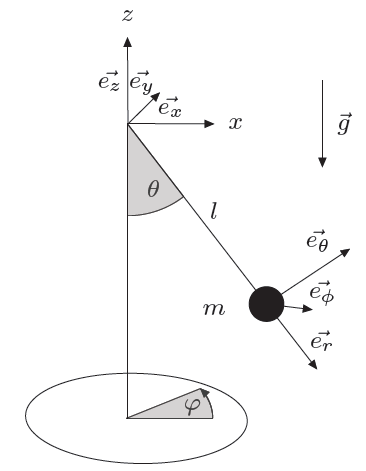
\includegraphics[width=0.35\textwidth]{péndulo_esférico.png}
\caption{Configuración geométrica de un \textbf{péndulo esférico}. La partícula de masa $m$
está unida al origen por una varilla rígida de longitud $l$ y se describe mediante los
ángulos esféricos $(\theta,\varphi)$ en presencia del campo gravitacional uniforme $\vec g$}
\label{fig:pendulo-esferico}
\end{figure}

Antes de escribir directamente el Lagrangiano y el Hamiltoniano, es útil entender
qué tipo de sistema mecánico estamos describiendo en términos de \textbf{grados de
libertad} y \textbf{restricciones}.  

En general, un sistema de \(N\) partículas en el espacio tridimensional requiere
\(3N\) coordenadas para especificar una configuración arbitraria.  
Si además existen \(k\) restricciones holonómicas independientes,
\[
f_{a}(x_{1},y_{1},z_{1},\dots,x_{N},y_{N},z_{N},t)=0,
\qquad a=1,\dots,k
\]
el número de \textbf{grados de libertad} queda reducido a
\[
n = 3N - k
\]

En el péndulo esférico tenemos únicamente \(N=1\) partícula en \(\mathbb{R}^{3}\),
de modo que sin restricciones habría \(3N = 3\) coordenadas independientes
\((x,y,z)\).  
La varilla rígida de longitud constante \(l\) impone la restricción holonómica

\[
x^{2} + y^{2} + z^{2} - l^{2} = 0
\]

que fija la partícula a la superficie de una esfera de radio \(l\).  
Esta es una sola ecuación, de modo que \(k=1\) y el número de grados de libertad
del sistema resulta

\[
n = 3N - k = 3 - 1 = 2
\]

Es decir, aunque el movimiento ocurre en el espacio tridimensional, la \textbf{configuración
del sistema} se puede describir completamente con sólo dos coordenadas
generalizadas.  
La Figura~\ref{fig:pendulo-esferico} sugiere escoger como tales precisamente los
ángulos esféricos \(\theta\) y \(\varphi\), que parametrizan la posición de la
partícula sobre la esfera de radio \(l\).  

\vspace{0.5cm}
\textbf{Elección de coordenadas y descripción geométrica}

Tomamos un sistema de referencia cartesiano \((x,y,z)\) con origen en el punto de
suspensión de la varilla.  
El eje \(z\) apunta verticalmente hacia arriba, mientras que el campo gravitacional
uniforme de la Tierra, \(\vec g\), apunta hacia abajo, como se indica en la
Figura~\ref{fig:pendulo-esferico}.  
En este sistema:

\begin{itemize}
  \item[$\bullet$] El ángulo \(\theta\) mide la inclinación de la varilla respecto al eje vertical \(z\)  
  \item[$\bullet$] El ángulo \(\varphi\) es el ángulo azimutal en el plano \(xy\), medido desde el eje \(x\)
\end{itemize}

La varilla rígida garantiza que la distancia del origen a la partícula es siempre
\(l\).  
En términos de \((\theta,\varphi)\), el vector de posición de la partícula viene dado por

\begin{equation}
\begin{split}
\vec r(\theta,\varphi)
&= x\,\hat e_{x} + y\,\hat e_{y} + z\,\hat e_{z} \\[4pt]
&= l\sin\theta\cos\varphi\,\hat e_{x}
 \;+\; l\sin\theta\sin\varphi\,\hat e_{y}
 \;+\; l\cos\theta\,\hat e_{z}
\end{split}\label{eq:posicion-pendulo-esferico}
\end{equation}

La condición \(x^{2}+y^{2}+z^{2}=l^{2}\) queda automáticamente satisfecha por la
expresión \eqref{eq:posicion-pendulo-esferico}, de modo que el vínculo se incorpora
al sistema a través de la elección de coordenadas.

\vspace{0.5cm}
\textbf{Energía cinética y potencial}

Para obtener la energía cinética calculamos la rapidez \(v = |\dot{\vec r}|\).  
El resultado estándar en coordenadas esféricas con radio fijo \(r=l\) nos dice que

\begin{equation}
\begin{split}
v^{2} &= l^{2}\bigl(\dot\theta^{2} + \sin^{2}\theta\,\dot\varphi^{2}\bigr)
\end{split}\label{eq:rapidez-pendulo-esferico}
\end{equation}

por lo que la energía cinética del péndulo esférico es

\begin{equation}
\begin{split}
T &= \frac{1}{2}\,m\,v^{2}
   = \frac{1}{2}\,m\,l^{2}\bigl(\dot\theta^{2} + \sin^{2}\theta\,\dot\varphi^{2}\bigr)
\end{split}\label{eq:T-pendulo-esferico}
\end{equation}

Para la energía potencial gravitacional tomamos como referencia \(U=0\) en el plano
horizontal \(z=0\).  
Como la coordenada vertical del punto material es \(z = l\cos\theta\), el potencial
viene dado por

\begin{equation}
\begin{split}
U(\theta) &= m g z = m g l\cos\theta
\end{split}\label{eq:U-pendulo-esferico}
\end{equation}

La configuración de mínima energía potencial se alcanza en \(\theta=\pi\), donde
la masa se encuentra por debajo del origen, mientras que \(\theta=0\) corresponde a
la posición “invertida”.

\vspace{0.5cm}
\textbf{Lagrangiano del péndulo esférico}

El Lagrangiano es la diferencia entre energía cinética y potencial, de modo que

\begin{equation}
\begin{split}
L(\theta,\varphi,\dot\theta,\dot\varphi)
&= T - U \\[4pt]
&= \frac{1}{2}\,m\,l^{2}\bigl(\dot\theta^{2} + \sin^{2}\theta\,\dot\varphi^{2}\bigr)
   \;-\; m g l\cos\theta
\end{split}\label{eq:L-pendulo-esferico}
\end{equation}

Esta expresión deja claro que el grado de libertad \(\varphi\) aparece únicamente a
través de su derivada temporal \(\dot\varphi\), lo cual anticipa que \(\varphi\) será
una \emph{coordenada cíclica} en la formulación Hamiltoniana.

\vspace{0.5cm}
\textbf{Momentos generalizados y espacio fase}

Las coordenadas generalizadas del sistema son \(\theta\) y \(\varphi\).  
Los momentos canónicos asociados se definen mediante

\[
p_{q_{i}} \equiv \frac{\partial L}{\partial \dot q_{i}}
\]

Aplicando esta definición al Lagrangiano \eqref{eq:L-pendulo-esferico} obtenemos

\begin{equation}
\begin{split}
p_{\theta} &\equiv \frac{\partial L}{\partial \dot\theta}
           = m l^{2}\dot\theta \\[4pt]
p_{\varphi} &\equiv \frac{\partial L}{\partial \dot\varphi}
            = m l^{2}\sin^{2}\theta\,\dot\varphi
\end{split}\label{eq:momentos-pendulo-esferico}
\end{equation}

El \textbf{espacio fase} del péndulo esférico está entonces parametrizado por las
cuatro variables canónicas \((\theta,\varphi,p_{\theta},p_{\varphi})\).  
Las relaciones \eqref{eq:momentos-pendulo-esferico} pueden invertirse para escribir
las velocidades en términos de los momentos,

\begin{equation}
\begin{split}
\dot\theta &= \frac{p_{\theta}}{m l^{2}} \\[4pt]
\dot\varphi &= \frac{p_{\varphi}}{m l^{2}\sin^{2}\theta}
\end{split}\label{eq:velocidades-en-funcion-de-momentos}
\end{equation}

lo cual será útil al construir el Hamiltoniano.

\vspace{0.5cm}
\textbf{Hamiltoniano del péndulo esférico}

El Hamiltoniano se define como la transformada de Legendre del Lagrangiano respecto
a las velocidades,

\[
H(\theta,\varphi,p_{\theta},p_{\varphi})
\equiv p_{\theta}\dot\theta + p_{\varphi}\dot\varphi - L
\]

Usando \eqref{eq:velocidades-en-funcion-de-momentos}, primero reescribimos la
energía cinética en función de los momentos. A partir de \eqref{eq:momentos-pendulo-esferico}
se tiene

\begin{equation}
\begin{split}
T &= \frac{1}{2}m l^{2}\dot\theta^{2}
   + \frac{1}{2}m l^{2}\sin^{2}\theta\,\dot\varphi^{2} \\[4pt]
  &= \frac{1}{2}\,\frac{p_{\theta}^{2}}{m l^{2}}
   + \frac{1}{2}\,\frac{p_{\varphi}^{2}}{m l^{2}\sin^{2}\theta}
\end{split}\label{eq:T-en-momentos}
\end{equation}

Como \(L = T - U\), la transformada de Legendre conduce al Hamiltoniano

\begin{equation}
\begin{split}
H(\theta,\varphi,p_{\theta},p_{\varphi})
&= T + U \\[4pt]
&= \frac{p_{\theta}^{2}}{2 m l^{2}}
 + \frac{p_{\varphi}^{2}}{2 m l^{2}\sin^{2}\theta}
 + m g l\cos\theta
\end{split}\label{eq:H-pendulo-esferico}
\end{equation}

Esta expresión \eqref{eq:H-pendulo-esferico} tiene una interpretación clara: el primer
término corresponde a la parte cinética asociada al “balanceo” en el ángulo
\(\theta\), el segundo a la contribución cinética debida a la rotación alrededor del
eje vertical (\(\varphi\)), y el último es la energía potencial gravitacional.  
Como el Lagrangiano no depende explícitamente del tiempo, el Hamiltoniano es una
\textbf{constante de movimiento} y coincide con la energía total del sistema.

\vspace{0.5cm}
\textbf{Ecuaciones de Hamilton}

Las ecuaciones de Hamilton para un sistema de dos grados de libertad se escriben como

\[
\dot q_{i} = \frac{\partial H}{\partial p_{i}},
\qquad
\dot p_{i} = -\,\frac{\partial H}{\partial q_{i}}
\]

En nuestro caso \(q_{1}=\theta\), \(q_{2}=\varphi\), con momentos
\(p_{1}=p_{\theta}\), \(p_{2}=p_{\varphi}\).  
A partir del Hamiltoniano \eqref{eq:H-pendulo-esferico} obtenemos primero las
ecuaciones para las coordenadas

\begin{equation}
\begin{split}
\dot\theta &= \frac{\partial H}{\partial p_{\theta}}
           = \frac{p_{\theta}}{m l^{2}} \\[4pt]
\dot\varphi &= \frac{\partial H}{\partial p_{\varphi}}
            = \frac{p_{\varphi}}{m l^{2}\sin^{2}\theta}
\end{split}\label{eq:ecuaciones-H-q}
\end{equation}

que coinciden exactamente con las relaciones ya obtenidas en
\eqref{eq:velocidades-en-funcion-de-momentos}.  
Para las ecuaciones de los momentos calculamos ahora las derivadas respecto a las
coordenadas. En primer lugar,

\begin{equation}
\begin{split}
\frac{\partial H}{\partial \theta}
&= \frac{\partial}{\partial\theta}
   \left[
     \frac{p_{\varphi}^{2}}{2 m l^{2}\sin^{2}\theta}
     + m g l\cos\theta
   \right] \\[4pt]
&= \frac{p_{\varphi}^{2}}{2 m l^{2}}
   \frac{\partial}{\partial\theta}\bigl(\sin^{-2}\theta\bigr)
   - m g l\sin\theta \\[4pt]
&= \frac{p_{\varphi}^{2}}{2 m l^{2}}
   \bigl(-2\sin^{-3}\theta\cos\theta\bigr)
   - m g l\sin\theta \\[4pt]
&= -\,\frac{p_{\varphi}^{2}\cos\theta}{m l^{2}\sin^{3}\theta}
   - m g l\sin\theta
\end{split}\label{eq:dH-dtheta}
\end{equation}

Por lo tanto, la ecuación de Hamilton para \(p_{\theta}\) queda

\begin{equation}
\begin{split}
\dot p_{\theta}
&= -\,\frac{\partial H}{\partial \theta} \\[4pt]
&= \frac{p_{\varphi}^{2}\cos\theta}{m l^{2}\sin^{3}\theta}
   + m g l\sin\theta
\end{split}\label{eq:ecuacion-H-ptheta}
\end{equation}

En cuanto a la coordenada \(\varphi\), el Hamiltoniano
\eqref{eq:H-pendulo-esferico} no depende explícitamente de ella, por lo que

\begin{equation}
\begin{split}
\frac{\partial H}{\partial \varphi} &= 0
\end{split}\label{eq:dH-dphi}
\end{equation}

y la ecuación correspondiente para \(p_{\varphi}\) se reduce simplemente a

\begin{equation}
\begin{split}
\dot p_{\varphi}
&= -\,\frac{\partial H}{\partial \varphi}
 = 0
\end{split}\label{eq:ecuacion-H-pphi}
\end{equation}

Así se ve con claridad que \(\varphi\) es una \textbf{coordenada cíclica} y su momento
canónico \(p_{\varphi}\) es una \textbf{constante de movimiento}.  
Geométricamente, \(p_{\varphi}\) está relacionado con la componente del momento
angular alrededor del eje vertical \(z\), de modo que el péndulo esférico conserva
su momento angular proyectado sobre ese eje.

\vspace{0.4cm}
\textbf{Comentario final sobre la dinámica}

El péndulo esférico queda completamente descrito en la formulación Hamiltoniana por
el Hamiltoniano

\begin{equation}
\begin{split}
H(\theta,\varphi,p_{\theta},p_{\varphi})
&= \frac{p_{\theta}^{2}}{2 m l^{2}}
 + \frac{p_{\varphi}^{2}}{2 m l^{2}\sin^{2}\theta}
 + m g l\cos\theta
\end{split}\label{eq:H-pendulo-esferico-resumen}
\end{equation}

junto con el sistema de ecuaciones de Hamilton formado por
\eqref{eq:ecuaciones-H-q}, \eqref{eq:ecuacion-H-ptheta} y
\eqref{eq:ecuacion-H-pphi}.  

Si en particular se considera el caso \(p_{\varphi}=0\), el movimiento queda
restringido a un plano fijo que contiene al eje vertical, y las ecuaciones se
reducen a las de un \textbf{péndulo plano} ordinario en la coordenada \(\theta\).  
Cuando \(p_{\varphi}\neq 0\), en cambio, el movimiento combina oscilaciones en
\(\theta\) con una precesión en el ángulo \(\varphi\), dando lugar a trayectorias
más ricas sobre la esfera de radio \(l\).  
Todo este comportamiento queda codificado, de manera compacta, en la estructura
del Hamiltoniano \eqref{eq:H-pendulo-esferico-resumen} y sus ecuaciones de Hamilton





\end{document}
